\documentclass[11pt,a4paper,oneside]{book}
%-- coding: UTF-8 --
\usepackage[UTF8]{ctex}
\usepackage{fontspec}
\defaultfontfeatures{Mapping=tex-text}
\usepackage{xunicode}%防止pdf乱码
%\usepackage{ccmap}%
\usepackage{xltxtra}
\usepackage{amsmath}
\usepackage{amsfonts}
\usepackage{amssymb}
\usepackage{graphicx}
\usepackage{amsthm}
\usepackage{array}
\usepackage{float}   %{H}
\usepackage{booktabs}  %\toprule[1.5pt]
\setcounter{secnumdepth}{4}
\usepackage{indentfirst} %首行缩进
\usepackage{tcolorbox} %彩色框框
\usepackage{graphicx}  %图片并排
\usepackage{subfigure} %图片并排
\usepackage{graphicx} %插入jpg
\usepackage[toc]{multitoc} %双列目录
\setcounter{secnumdepth}{4}		%增加编号深度
\setcounter{tocdepth}{4}		%增加目录深度
\usepackage{hyperref}     %生成pdf书签
\hypersetup{hidelinks,
	colorlinks=true,
	allcolors=black,
	pdfstartview=Fit,
	breaklinks=true
}       %去掉目录的红色框框
%===================%插入代码需要的控制
\usepackage{listings}
\usepackage{xcolor}
\setmonofont{Consolas}%字体
\lstset{%
	numbers=left,
	numberstyle=\tt\tiny,%
	showstringspaces=false,
	showspaces=false,%
	tabsize=4,%
	frame=lines,%
	basicstyle=\tt\small,%
	keywordstyle=\color{ blue!70}\bfseries,%
	identifierstyle=,%
	commentstyle=\color{red!50!green!50!blue!50},%\itshape,%
	stringstyle=\color{black},%
	breaklines=true
}
%===================%
\usepackage[left=2cm,right=2cm,top=2cm,bottom=2cm]{geometry}
\newtheorem{theorem}{定理}
\newtheorem{definition}{定义}
\newtheorem{e}{例}
\title{\Huge NOTE on Multiple statistical analysis with R}
\author{zy}
\date{\today}

\begin{document}
\maketitle
\tableofcontents  %目录
\chapter{多元统计分析与R}
\begin{lstlisting}[language=r]
> help.start()
如果什么都不发生的话,你应该自己打开‘http://127.0.0.1:16624/doc/html/index.html’
> help("seq")
> help(seq)
> ?seq
> ?"seq"
\end{lstlisting}
\begin{lstlisting}[language=r]
> help.search("multivariate normal")
> ??"multivariate normal"
\end{lstlisting}
\begin{lstlisting}[language=r]
> x1<-seq(2,6,by=1)
> x1
[1] 2 3 4 5 6
> x3<-rep(2:4,2)
> x3
[1] 2 3 4 2 3 4
> c4
[1] 2 3 4 5 6 2 3 4 2 3 4
> d4<-cbind(x1,x3)
Warning message:
In cbind(x1, x3) :
number of rows of result is not a multiple of vector length (arg 1)

#说明cbind只能合并维数相同的向量 (按行合并rbind也一样)
\end{lstlisting}
\begin{lstlisting}[language=r]
> A<-matrix(1,2,2)
> A
[,1] [,2]
[1,]    1    1
[2,]    1    1
> B<-diag(3)
> B
[,1] [,2] [,3]
[1,]    1    0    0
[2,]    0    1    0
[3,]    0    0    1
> D<-diag(c(2,3,4))
> D
[,1] [,2] [,3]
[1,]    2    0    0
[2,]    0    3    0
[3,]    0    0    4
> x2<-c(1,2,3,4,5)
> E<-rbind(x1,x2)
> E
[,1] [,2] [,3] [,4] [,5]
x1    2    3    4    5    6
x2    1    2    3    4    5
\end{lstlisting}
\begin{lstlisting}[language=r]
> z.df<-data.frame(x1,x2)
> z.df
x1 x2
1  2  1
2  3  2
3  4  3
4  5  4
5  6  5
\end{lstlisting}

\section{一个回归分析的例子}
\begin{figure}[H]
	\centering
	\includegraphics[width=0.8\textwidth]{screenshot035}
\end{figure}
\begin{lstlisting}[language=r]
> data1<-read.csv("E:/4.多元统计分析/图书馆借的书 代码/多元统计分析——基于R(第2版) R-data/eg1.1.csv",header=TRUE)
> data1
district        x        y
1    北  京 52859.17 36642.00
2    天  津 34101.35 26229.52
3    河  北 26152.16 17586.62
4    山  西 25827.72 15818.61
5    内蒙古 30594.10 21876.47
6    辽  宁 31125.73 21556.72
7    吉  林 24900.86 17972.62
8    黑龙江 24202.62 17152.07
9    上  海 52961.86 36946.12
10   江  苏 37173.48 24966.04
11   浙  江 43714.48 28661.27
12   安  徽 26935.76 17233.53
13   福  建 33275.34 23520.19
14   江  西 26500.12 16731.81
15   山  东 31545.27 19853.77
16   河  南 25575.61 17154.30
17   湖  北 27051.47 18192.28
18   湖  南 28838.07 19501.37
19   广  东 34757.16 25673.08
20   广  西 26415.87 16321.16
21   海  南 26356.42 18448.35
22   重  庆 27238.84 19742.29
23   四  川 26205.25 19276.85
24   贵  州 24579.64 16914.20
25   云  南 26373.23 17674.99
26   西  藏 25456.63 17022.01
27   陕  西 26420.21 18463.87
28   甘  肃 23767.08 17450.86
29   青  海 24542.35 19200.65
30   宁  夏 25186.01 18983.88
31   新  疆 26274.66 19414.74

> cor(data1$x,data1$y) #相关系数
[1] 0.9736406
> plot(y~x,data=data1) #x和y的散点图
\end{lstlisting}
\begin{figure}[H]
	\centering
	\includegraphics[width=0.8\textwidth]{screenshot036}
\end{figure}
\begin{lstlisting}[language=r]
> lm.regression<-lm(y~x,data=data1) #求解线性回归方程
> summary(lm.regression)  #输出回归分析的结果

Call:
lm(formula = y ~ x, data = data1)

Residuals:
    Min      1Q  Median      3Q     Max 
-2099.8  -629.8   138.5   772.7  2628.6 

Coefficients:
             Estimate Std. Error t value Pr(>|t|)    
(Intercept) 179.43046  920.59493   0.195    0.847    
x             0.68682    0.02988  22.988   <2e-16 ***
---
Signif. codes:  0 ‘***’ 0.001 ‘**’ 0.01 ‘*’ 0.05 ‘.’ 0.1 ‘ ’ 1

Residual standard error: 1238 on 29 degrees of freedom
Multiple R-squared:  0.948,	Adjusted R-squared:  0.9462 
F-statistic: 528.4 on 1 and 29 DF,  p-value: < 2.2e-16

> abline(a=179.43046,b=0.68682)
\end{lstlisting}
\begin{figure}[H]
	\centering
	\includegraphics[width=0.8\textwidth]{screenshot037}
\end{figure}
\begin{lstlisting}[language=r]
#求lm.regression回归参数的95%置信区间
> confint(lm.regression,level = .95)  
                    2.5 %       97.5 %
(Intercept) -1703.3975771 2062.2584891
x               0.6257138    0.7479274

#求预测值和预测区间
> x0<-data.frame(x=30000)
> predict(lm.regression,x0,interval = "prediction",level = 0.95)
       fit      lwr      upr
1 20784.05 18212.12 23355.98
\end{lstlisting}
\section{矩阵代数回顾}
生成由正态分布N(-1,1),N(1,1)随机数组成的两个矩阵$ A_{(3,4)},B_{(4,3)} $
\begin{lstlisting}[language=r]
> set.seed(1010)
> (A <- matrix(rnorm(12,-1,1),3,4))
           [,1]       [,2]       [,3]      [,4]
[1,] -0.8684591 -0.5799253  0.9387253 -1.544553
[2,] -1.8979099 -1.2884597 -3.3609830 -1.195908
[3,]  0.3519446  0.3645614 -1.5941141 -1.830073
> (B <- matrix(rnorm(12,1,1),4,3))
           [,1]       [,2]      [,3]
[1,] -0.4353805 0.18132106 1.0848711
[2,]  0.9239290 1.20464153 1.7148650
[3,]  1.7258680 0.04758697 0.0337592
[4,]  0.2122666 0.03419967 1.4623014
> (2*A+3*t(B))
          [,1]     [,2]      [,3]       [,4]
[1,] -3.043060 1.611936  7.055055 -2.4523056
[2,] -3.251857 1.037005 -6.579205 -2.2892176
[3,]  3.958502 5.873718 -3.086951  0.7267572
> (C <- A%*%B)
          [,1]       [,2]      [,3]
[1,]  1.134559 -0.8642241 -4.163571
[2,] -6.418597 -2.0971018 -6.130764
[3,] -2.956095  0.3645337 -1.722947
\end{lstlisting}

计算C的行列式;输出$ C^{-1}C $,它应该等于单位矩阵,但由于浮点运算,结果不大可能刚好是0和1组成的单位矩阵
\begin{lstlisting}[language=r]
> det(C)
[1] 36.08275
> (cni <- solve(C))
           [,1]        [,2]        [,3]
[1,]  0.1620737 -0.08332996 -0.09514454
[2,]  0.1957783 -0.39527741  0.93340992
[3,] -0.2366512  0.05933981 -0.21967263
> cni%*%C
              [,1]          [,2]          [,3]
[1,]  1.000000e+00 -1.387779e-17 -1.110223e-16
[2,] -4.440892e-16  1.000000e+00 -2.220446e-16
[3,]  1.110223e-16  4.163336e-17  1.000000e+00
> dim(C)
[1] 3 3
\end{lstlisting}

随机产生$ 25\times 4 $矩阵X; 计算X的相关阵; 解X的相关阵的特征值问题; 验证特征向量组成正交矩阵;验证X相关阵的对角线元素的和(迹)等于其特征根的和.
\begin{lstlisting}[language=r]
> set.seed(1010)
> (X <- matrix(rnorm(100),25,4))
            [,1]        [,2]         [,3]         [,4]
[1,]  0.13154085  0.73876017  1.834489903 -2.349238899
[2,] -0.89790987 -0.31882166 -0.772763578 -0.223386083
[3,]  1.35194461 -1.05196788 -1.140738390 -0.144527545
[4,]  0.42007469 -0.28592085 -0.371532658 -0.007959542
[5,] -0.28845968 -1.83786541  0.023858412  2.124718712
[6,]  1.36456136 -1.03990318 -0.179129521  1.229289823
[7,]  1.93872531  1.92416803  0.930124039 -1.759589232
[8,] -2.36098302 -0.14718335  1.589100476  1.745634639
[9,] -0.59411413  0.32966774 -0.118753321 -0.484385941
[10,] -0.54455270 -1.03558049  1.618127294  0.508974866
[11,] -0.19590829  0.35150814  1.567786166 -1.363468851
[12,] -0.83007345 -0.27533224  0.644977071 -0.667703109
[13,] -1.43538053 -0.38736785  0.853215243 -1.553401769
[14,] -0.07607103 -0.57081846 -0.360481960  0.899507827
[15,]  0.72586799 -0.99120874  0.517182812 -2.629247852
[16,] -0.78773341 -0.38047536 -1.978282908 -0.592126313
[17,] -0.81867894  0.41397430  0.562623033  0.672648804
[18,]  0.20464153 -0.08662838 -0.437089345 -1.306310026
[19,] -0.95241303  0.68663415 -0.765279280 -0.047702968
[20,] -0.96580033 -0.69431272 -0.005079319 -1.143892432
[21,]  0.08487109  0.15716619  0.546463286 -0.527634736
[22,]  0.71486499  0.32590725 -0.313698940 -1.079384672
[23,] -0.96624080 -0.58511242 -0.751924345 -0.738360314
[24,]  0.46230137  0.33682643  1.046418792  1.167064405
[25,] -0.68605062  1.31967884 -0.408624843 -1.879321895
> (XC <- cor(X))
            [,1]        [,2]        [,3]        [,4]
[1,]  1.00000000  0.09692075 -0.07014491 -0.17990011
[2,]  0.09692075  1.00000000  0.20620831 -0.43280660
[3,] -0.07014491  0.20620831  1.00000000 -0.04410169
[4,] -0.17990011 -0.43280660 -0.04410169  1.00000000

> (a <- eigen(XC))
eigen() decomposition
$values
[1] 1.5460956 1.0988869 0.8205692 0.5344484

$vectors
           [,1]       [,2]       [,3]        [,4]
[1,] -0.2941782  0.6515723  0.6954248  0.07278099
[2,] -0.6589958 -0.1600336 -0.2027558  0.70640209
[3,] -0.2627723 -0.7235443  0.5917942 -0.23919457
[4,]  0.6404174 -0.1622543  0.3536299  0.66218198

> round(t(a$vectors)%*%a$vectors,14)
     [,1] [,2] [,3] [,4]
[1,]    1    0    0    0
[2,]    0    1    0    0
[3,]    0    0    1    0
[4,]    0    0    0    1
> (tr <- sum(a$values))
[1] 4
> sum(diag(XC))
[1] 4
\end{lstlisting}

\chapter{多元正态分布}
\section{多元线性模型}
\begin{figure}[H]
	\centering
	\includegraphics[width=0.8\textwidth]{screenshot038}
\end{figure}
\begin{lstlisting}[language=r]
> data2<-read.csv("E:/4.多元统计分析/图书馆借的书 代码/多元统计分析——基于R(第2版) R-data/eg2.1.csv",header=TRUE)
> data2
    y x1 x2 x3 x4 x5
1  85 83 86 90 90 76
2  90 92 88 87 92 80
3  78 70 76 73 85 90
4  80 72 81 82 90 88
5  86 80 90 88 73 78
6  92 82 93 90 88 80
7  77 83 84 80 90 86
8  69 68 75 66 85 80
9  75 80 78 78 86 83
10 50 62 76 55 85 78
11 60 78 83 63 80 75
12 95 90 87 92 90 85
13 83 85 86 85 91 80
14 82 88 85 87 87 84
15 66 70 74 65 88 85
16 81 85 81 80 86 73
17 92 83 85 90 85 80
18 78 84 82 73 90 83
19 45 60 65 60 86 78
20 76 80 81 75 80 75
21 88 85 82 86 85 80
22 82 80 81 86 87 90
23 83 76 79 80 80 92
24 75 80 74 82 89 87
25 90 85 90 88 88 91
26 65 75 73 68 82 80
27 74 80 72 78 80 83
28 80 82 71 83 76 76
29 84 80 78 87 80 82
30 65 72 68 70 82 77
31 72 82 77 75 76 75
32 70 86 85 78 84 89
33 79 75 67 85 75 82
34 86 83 80 88 80 85
35 62 78 65 60 85 88
36 87 80 83 85 78 83

> lm.exam<-lm(y~x1+x2+x3+x4+x5,data=data2)
> summary(lm.exam)

Call:
lm(formula = y ~ x1 + x2 + x3 + x4 + x5, data = data2)

Residuals:
     Min       1Q   Median       3Q      Max 
-10.0696  -1.7983  -0.1535   2.9361   6.8726 

Coefficients:
             Estimate Std. Error t value Pr(>|t|)    
(Intercept) -32.73534   15.35701  -2.132   0.0413 *  
x1            0.16271    0.15031   1.082   0.2877    
x2            0.22784    0.13835   1.647   0.1100    
x3            0.88116    0.11108   7.933 7.46e-09 ***
x4           -0.05136    0.15476  -0.332   0.7423    
x5            0.16887    0.14376   1.175   0.2494    
---
Signif. codes:  0 ‘***’ 0.001 ‘**’ 0.01 ‘*’ 0.05 ‘.’ 0.1 ‘ ’ 1

Residual standard error: 4.021 on 30 degrees of freedom
Multiple R-squared:  0.8945,	Adjusted R-squared:  0.877 
F-statistic: 50.89 on 5 and 30 DF,  p-value: 9.359e-14
\end{lstlisting}
由F检验知方程显著,但是t检验中只有常数项和x3显著.故要进行变量选择.

\section{变量选择}
\begin{lstlisting}[language=r]
> lm.exam.step<-step(lm.exam,direction = "both") #逐步回归
Start:  AIC=105.63
y ~ x1 + x2 + x3 + x4 + x5

       Df Sum of Sq     RSS    AIC
- x4    1      1.78  486.83 103.76
- x1    1     18.95  503.99 105.01
- x5    1     22.31  507.36 105.25
<none>               485.05 105.63
- x2    1     43.85  528.90 106.74
- x3    1   1017.44 1502.49 144.33

Step:  AIC=103.76
y ~ x1 + x2 + x3 + x5

       Df Sum of Sq     RSS    AIC
- x1    1     17.91  504.73 103.06
- x5    1     20.57  507.40 103.25
<none>               486.83 103.76
- x2    1     42.99  529.81 104.80
+ x4    1      1.78  485.05 105.63
- x3    1   1112.96 1599.79 144.59

Step:  AIC=103.06
y ~ x2 + x3 + x5

       Df Sum of Sq     RSS    AIC
- x5    1     17.40  522.14 102.28
<none>               504.73 103.06
+ x1    1     17.91  486.83 103.76
+ x4    1      0.74  503.99 105.01
- x2    1     70.76  575.50 105.78
- x3    1   1848.49 2353.23 156.48

Step:  AIC=102.28
y ~ x2 + x3

       Df Sum of Sq     RSS    AIC
<none>               522.14 102.28
+ x5    1     17.40  504.73 103.06
+ x1    1     14.74  507.40 103.25
+ x4    1      0.25  521.89 104.26
- x2    1     66.64  588.78 104.60
- x3    1   1953.30 2475.43 156.30
\end{lstlisting}
故y关于x2,x3回归最优.
\begin{lstlisting}[language=r]
> summary(lm.exam.step)

Call:
lm(formula = y ~ x2 + x3, data = data2)

Residuals:
     Min       1Q   Median       3Q      Max 
-10.4395  -2.5508  -0.4459   2.7367   7.2345 

Coefficients:
             Estimate Std. Error t value Pr(>|t|)    
(Intercept) -18.84290    7.58902  -2.483   0.0183 *  
x2            0.24923    0.12144   2.052   0.0481 *  
x3            0.96804    0.08713  11.111 1.09e-12 ***
---
Signif. codes:  0 ‘***’ 0.001 ‘**’ 0.01 ‘*’ 0.05 ‘.’ 0.1 ‘ ’ 1

Residual standard error: 3.978 on 33 degrees of freedom
Multiple R-squared:  0.8865,	Adjusted R-squared:  0.8796 
F-statistic: 128.8 on 2 and 33 DF,  p-value: 2.566e-16
\end{lstlisting}

\section{回归诊断}
\subsection{残差分析和异常点分析}
\begin{lstlisting}[language=r]
> y.res<-residuals(lm.exam)  #模型lm.exam的普通残差
> y.res
1            2            3            4            5 
-2.87977886   2.27086619   6.87264683   0.07212446  -1.75155533 
6            7            8            9           10 
1.90985899  -3.30117393   6.28269511  -1.38251878  -1.93838930 
11           12           13           14           15 
-2.93613882   2.47127763  -1.42351275  -5.32703672   3.37601943 
16           17           18           19           20 
3.04675134   3.41579007   4.66651141  -8.46115431   2.62020764 
21           22           23           24           25 
3.29852573  -3.24602265   3.45020172  -4.51717857   0.01002824 
26           27           28           29           30 
-0.31700658  -1.32363971   1.14960631  -0.45225026   0.05461402 
31           32           33           34           35 
-0.99929640 -10.06959676  -0.62692999  -0.78382675   3.87000483 
36 
2.89927651

> y.rst<-rstandard(lm.exam.step)  #计算lm.exam.step模型的标准化残差
> y.rst
1           2           3           4           5           6 
-1.22647949  0.70123348  1.85465439 -0.18487397 -0.73157547  0.14591132 
7           8           9          10          11          12 
-0.65165378  1.37662024 -0.28171298 -0.96473838 -0.79862247  0.81284419 
13          14          15          16          17          18 
-0.48393343 -1.17668588  0.91337716  0.56438902  0.65876689  1.49006874 
19          20          21          22          23          24 
-2.87121739  0.52710268  0.81076269 -0.66801351  1.20184149 -1.04020189 
25          26          27          28          29          30 
0.32282704 -0.04616114 -0.15912001  0.21602487 -0.21306706 -0.23026109 
31          32          33          34          35          36 
-0.24302334 -2.03567204 -0.33183300 -0.07354893  1.80438009  0.73702932 

> y.fit<-predict(lm.exam.step)  #求模型lm.exam.step的预测值
> y.fit
1        2        3        4        5        6        7        8 
89.71447 87.30882 70.76550 80.72400 88.77532 91.45909 79.53562 63.74000 
9       10       11       12       13       14       15       16 
76.10415 53.34082 62.82975 91.89977 84.87428 86.56112 62.52273 78.78793 
17       18       19       20       21       22       23       24 
89.46523 72.26089 55.43946 73.94774 84.84539 84.59615 78.28946 78.97938 
25       26       27       28       29       30       31       32 
88.77532 65.17762 74.60876 79.19972 84.81650 65.86753 72.95081 77.84878 
33       34       35       36 
80.13887 86.28300 55.43946 84.12658 

> plot(y.res~y.fit)  #残差图
> plot(y.rst~y.fit)
\end{lstlisting}
\begin{figure}[H]
	\centering
	\includegraphics[width=0.7\textwidth]{screenshot039}
\end{figure}
\begin{figure}[H]
	\centering
	\includegraphics[width=0.7\textwidth]{screenshot040}
\end{figure}
由图,残差的分布有随预测值增大而减小的趋势,所以同方差的假设可能不成立.可以通过box-cox变换对因变量作适当变换来解决方差非齐问题.
\begin{lstlisting}[language=r]
> lm.exam.step.new<-update(lm.exam.step,log(.)~.)  #对模型进行对数变换
> y.rst<-rstandard(lm.exam.step.new)
> y.fit<-predict(lm.exam.step.new)
> plot(y.rst~y.fit)
\end{lstlisting}
\begin{figure}[H]
	\centering
	\includegraphics[width=0.6\textwidth]{screenshot041}
\end{figure}

变换后的散点图有所改善,但是19还是异常点,我们去掉19号观测值,重复上述回归分析的步骤和残差分析的过程,可以得到新的标准残差图:
\begin{lstlisting}[language=r]
> lm.exam<-lm(log(y)~x1+x2+x3+x4+x5,data=data2[-c(19),])
> lm.step<-step(lm.exam,direction="both")
Start:  AIC=-204.01
log(y) ~ x1 + x2 + x3 + x4 + x5

       Df Sum of Sq      RSS     AIC
- x4    1  0.000170 0.073248 -205.92
- x1    1  0.000500 0.073578 -205.77
- x2    1  0.001197 0.074275 -205.44
- x5    1  0.001694 0.074771 -205.20
<none>              0.073078 -204.00
- x3    1  0.207981 0.281059 -158.86

Step:  AIC=-205.92
log(y) ~ x1 + x2 + x3 + x5

       Df Sum of Sq      RSS     AIC
- x1    1  0.000644 0.073893 -207.62
- x2    1  0.001797 0.075045 -207.08
- x5    1  0.002437 0.075685 -206.78
<none>              0.073248 -205.92
+ x4    1  0.000170 0.073078 -204.00
- x3    1  0.222573 0.295821 -159.07

Step:  AIC=-207.62
log(y) ~ x2 + x3 + x5

       Df Sum of Sq     RSS     AIC
- x5    1   0.00216 0.07605 -208.61
- x2    1   0.00265 0.07654 -208.38
<none>              0.07389 -207.62
+ x1    1   0.00064 0.07325 -205.92
+ x4    1   0.00031 0.07358 -205.77
- x3    1   0.33826 0.41215 -149.46

Step:  AIC=-208.61
log(y) ~ x2 + x3

       Df Sum of Sq     RSS     AIC
- x2    1   0.00228 0.07833 -209.58
<none>              0.07605 -208.61
+ x5    1   0.00216 0.07389 -207.62
+ x4    1   0.00106 0.07499 -207.10
+ x1    1   0.00036 0.07569 -206.78
- x3    1   0.35283 0.42887 -150.07

Step:  AIC=-209.58
log(y) ~ x3

       Df Sum of Sq     RSS     AIC
<none>              0.07833 -209.58
+ x4    1   0.00231 0.07601 -208.63
+ x2    1   0.00228 0.07605 -208.61
+ x5    1   0.00178 0.07654 -208.38
+ x1    1   0.00102 0.07731 -208.04
- x3    1   0.58208 0.66041 -136.96
> y.rst<-rstandard(lm.step)
> y.fit<-predict(lm.step)
> plot(y.rst~y.fit)
\end{lstlisting}
\begin{figure}[H]
	\centering
	\includegraphics[width=0.7\textwidth]{screenshot042}
\end{figure}

\subsection{回归诊断:一般方法}
\begin{lstlisting}[language=r]
#对lm.exam.step.new进行回归诊断

> par(mfrow=c(2,2)) #在一个2x2网格中创建4个绘图区
> plot(lm.exam.step.new)  #绘制模型诊断图
\end{lstlisting}
\begin{figure}[H]
	\centering
	\includegraphics[width=\textwidth]{screenshot043}
\end{figure}

以上给出了逐步回归模型lm.xam.step.new的四个回归诊断图:

1. 残差-拟合图:点基本呈随机分布模式

2. 正态QQ图:点基本落在直线上,说明残差服从正态分布.

3. 大小-位置图和残差-杠杆图中第19号点偏离中心位置最远,说明19可能是异常点或者强影响点.
\begin{lstlisting}[language=r]
> influence.measures(lm.exam.step.new)  #计算各个观测值的诊断统计量
Influence measures of
lm(formula = log(y) ~ x2 + x3, data = data2) :

  dfb.1_    dfb.x2    dfb.x3    dffit cov.r   cook.d    hat inf
1   0.172353 -0.052013 -1.36e-01 -0.29171 1.052 2.82e-02 0.0662    
2  -0.078941  0.062234  6.53e-03  0.11045 1.160 4.17e-03 0.0691    
3   0.196029 -0.049262 -1.17e-01  0.37308 0.836 4.31e-02 0.0383    
4   0.000755 -0.000092 -1.18e-03 -0.00514 1.131 9.10e-06 0.0307    
5   0.158595 -0.132904  5.82e-04 -0.20447 1.159 1.42e-02 0.0904    
6   0.050075 -0.042979  2.40e-03 -0.06003 1.260 1.24e-03 0.1314    
7   0.029049 -0.041520  2.08e-02 -0.07054 1.134 1.70e-03 0.0431    
8   0.221339  0.062547 -3.07e-01  0.43692 0.967 6.13e-02 0.0773    
9  -0.001287  0.000895 -2.66e-04 -0.00456 1.130 7.15e-06 0.0291    
10 -0.244874 -0.373578  7.68e-01 -0.82996 1.190 2.22e-01 0.2421    
11  0.014319 -0.193460  2.46e-01 -0.27029 1.346 2.49e-02 0.2065   *
12 -0.037878  0.010399  3.07e-02  0.06036 1.188 1.25e-03 0.0806    
13  0.049535 -0.040469 -3.55e-03 -0.08053 1.144 2.22e-03 0.0520    
14  0.119031 -0.054536 -7.04e-02 -0.21645 1.064 1.57e-02 0.0504    
15  0.178766  0.024975 -2.15e-01  0.31461 1.084 3.29e-02 0.0840    
16 -0.012867  0.018741 -2.27e-03  0.10445 1.092 3.71e-03 0.0291    
17 -0.031017  0.003645  3.30e-02  0.06027 1.166 1.25e-03 0.0643    
18 -0.042282  0.255166 -2.86e-01  0.40524 0.936 5.24e-02 0.0624    
19 -2.023566  1.001611  7.40e-01 -2.21899 0.232 9.50e-01 0.1645   *
20 -0.006664  0.071366 -8.14e-02  0.14712 1.093 7.33e-03 0.0419    
21 -0.031706 -0.011930  6.08e-02  0.11639 1.115 4.61e-03 0.0432    
22  0.018693  0.027593 -6.80e-02 -0.11345 1.120 4.39e-03 0.0454    
23  0.024368 -0.033773  3.84e-02  0.18922 1.012 1.19e-02 0.0291    
24 -0.095201  0.160717 -1.33e-01 -0.20907 1.128 1.48e-02 0.0750    
25 -0.021612  0.018111 -7.93e-05  0.02786 1.205 2.67e-04 0.0904    
26  0.028025 -0.007627 -1.77e-02  0.03967 1.170 5.41e-04 0.0643    
27  0.008092 -0.009900  5.70e-03  0.01251 1.185 5.38e-05 0.0749    
28  0.046310 -0.078289  6.28e-02  0.09025 1.258 2.80e-03 0.1326    
29 -0.006199  0.036056 -4.75e-02 -0.06151 1.176 1.30e-03 0.0719    
30 -0.016798  0.013639 -1.56e-03 -0.01911 1.222 1.26e-04 0.1029    
31  0.002796 -0.000831 -1.33e-03  0.00658 1.133 1.49e-05 0.0326    
32  0.158439 -0.279129  1.92e-01 -0.38083 0.952 4.66e-02 0.0605    
33 -0.080807  0.140284 -1.13e-01 -0.15234 1.464 7.96e-03 0.2556   *
34  0.003073  0.018428 -3.20e-02 -0.04254 1.169 6.22e-04 0.0643    
35  0.694033 -0.343528 -2.54e-01  0.76106 1.008 1.82e-01 0.1645    
36 -0.041692  0.012644  3.72e-02  0.10921 1.111 4.06e-03 0.0394    
\end{lstlisting}

influence.measures给出了诊断统计量DFBETAS,DFFITS,协方差比(cov.r),库克距离,帽子阵的值.注意到11,19,33被诊断为强影响点.

\section{回归预测}
\begin{lstlisting}[language=r]
> preds<-data.frame(x2=80,x3=90)
> predict(lm.exam.step,newdata = preds,interval = "prediction",level = 0.95)
       fit      lwr      upr
1 88.21907 79.79748 96.64067
\end{lstlisting}
interval = "prediction"表示要给出置信区间.
\chapter{广义线性模型}
\section{广义线性模型的定义}
多元线性模型的重要假定是因变量为连续型变量,通常假定服从正态分布.

如果结果变量为类型变量如二分类多分类变量,或者结果变量为计数型变量,我们可以考虑用广义线性模型.

定义见书.
\section{Logistic模型}
设y服从参数为p的二项分布,则$ \mu=\mathbb{E}(y)=p $,采用逻辑连接函数,即\[logit(p)=\ln\frac{p}{1-p}=X\beta\]
这个广义线性模型称为logistic模型.
\begin{e}
数据集给出了某城市48个家庭的调查数据,y是分类变量(是否有买房),x1是家庭收入,x2是家中是否有孩子.根据这个数据集建立logistic回归模型并估计年收入为20万元,家里有孩子的家庭有购买住房的可能性.
\end{e}
\begin{lstlisting}[language=r]
> data3<-read.csv("E:/4.多元统计分析/图书馆借的书 代码/多元统计分析——基于R(第2版) R-data/eg3.1.csv",header=TRUE)
> data3
   x1 x2 y
1  20  1 1
2  30  1 1
3  10  0 0
4  22  0 1
5   8  0 0
......
45 23  0 0
46 26  1 1
47 10  0 0
48 36  1 1

> glm.logit<-glm(y~x1+x2,family = binomial(link=logit),data=data3)
> summary(glm.logit)

Call:
glm(formula = y ~ x1 + x2, family = binomial(link = logit), data = data3)

Deviance Residuals: 
     Min        1Q    Median        3Q       Max  
-2.30297  -0.19832   0.02283   0.20251   1.59258  

Coefficients:
            Estimate Std. Error z value Pr(>|z|)   
(Intercept) -7.53115    2.56352  -2.938  0.00331 **
x1           0.43956    0.13864   3.170  0.00152 **
x2          -0.08103    1.24747  -0.065  0.94821   
---
Signif. codes:  0 ‘***’ 0.001 ‘**’ 0.01 ‘*’ 0.05 ‘.’ 0.1 ‘ ’ 1

(Dispersion parameter for binomial family taken to be 1)

Null deviance: 61.105  on 47  degrees of freedom
Residual deviance: 17.643  on 45  degrees of freedom
AIC: 23.643

Number of Fisher Scoring iterations: 8
\end{lstlisting}
注意到x2对应的p值比较大,即x2不显著,所以考虑采用逐步回归.
\begin{lstlisting}[language=r]
> glm.step<-step(glm.logit)
Start:  AIC=23.64
y ~ x1 + x2

       Df Deviance    AIC
- x2    1   17.647 21.647
<none>      17.643 23.643
- x1    1   59.008 63.008

Step:  AIC=21.65
y ~ x1

       Df Deviance    AIC
<none>      17.647 21.647
- x1    1   61.105 63.105

> summary(glm.step)

Call:
glm(formula = y ~ x1, family = binomial(link = logit), data = data3)

Deviance Residuals: 
Min        1Q    Median        3Q       Max  
-2.28859  -0.19703   0.02276   0.20400   1.60887  

Coefficients:
Estimate Std. Error z value Pr(>|z|)   
(Intercept)  -7.5682     2.5101  -3.015  0.00257 **
x1            0.4396     0.1387   3.169  0.00153 **
---
Signif. codes:  0 ‘***’ 0.001 ‘**’ 0.01 ‘*’ 0.05 ‘.’ 0.1 ‘ ’ 1

(Dispersion parameter for binomial family taken to be 1)

Null deviance: 61.105  on 47  degrees of freedom
Residual deviance: 17.647  on 46  degrees of freedom
AIC: 21.647

Number of Fisher Scoring iterations: 8
\end{lstlisting}
注意:回归系数对应的p值越小越显著,*表示在5$ \% $水平上显著,**表示在1$ \% $水平上显著,***表示在0.1$ \% $水平上显著.

容易看出,回归模型的回归系数在1$ \% $水平上显著,于是得回归模型为:
\[ln\frac{\hat{p}}{1-\hat{p}}=-7.57+0.44x_1\]

如果要预测年收入为20万元(x1=20),家里有孩子(x2=1)的家庭有购买住房的可能性:

\begin{lstlisting}[language=r]
> yp<-predict(glm.step,data.frame(x1=20))
> p.fit<-exp(yp)/(1+exp(yp))
> p.fit
1 
0.7728122 
\end{lstlisting}

\section{Probit模型}
设y服从参数为p的二项分布,则$ \mu=\mathbb{E}(y)=p $,采用Probit连接函数,即\[g(\mu)=probit(p)=\Phi^{-1}(p)=X\beta\]
其中$ \Phi $是标准正态分布函数,这个广义线性模型称为Probit模型.
\begin{e}
同例1,建立Probit回归模型.
\end{e}
\begin{lstlisting}[language=r]
> glm.probit<-glm(y~x1+x2,family = binomial(link = probit),data=data3)
Warning message:
glm.fit:拟合機率算出来是数值零或一 
> summary(glm.probit)

Call:
glm(formula = y ~ x1 + x2, family = binomial(link = probit), 
data = data3)

Deviance Residuals: 
     Min        1Q    Median        3Q       Max  
-2.24700  -0.15143   0.00179   0.17737   1.60504  

Coefficients:
             Estimate Std. Error z value Pr(>|z|)    
(Intercept) -4.344942   1.326518  -3.275  0.00105 ** 
x1           0.249972   0.069616   3.591  0.00033 ***
x2           0.008167   0.691290   0.012  0.99057    
---
Signif. codes:  0 ‘***’ 0.001 ‘**’ 0.01 ‘*’ 0.05 ‘.’ 0.1 ‘ ’ 1

(Dispersion parameter for binomial family taken to be 1)

Null deviance: 61.105  on 47  degrees of freedom
Residual deviance: 17.349  on 45  degrees of freedom
AIC: 23.349

Number of Fisher Scoring iterations: 9
\end{lstlisting}
注意到x2对应的p值比较大,即x2不显著,所以考虑采用逐步回归.
\begin{lstlisting}[language=r]
> glm.p.step<-step(glm.probit)
Start:  AIC=23.35
y ~ x1 + x2

       Df Deviance    AIC
- x2    1   17.349 21.349
<none>      17.349 23.349
- x1    1   59.008 63.008

Step:  AIC=21.35
y ~ x1

       Df Deviance    AIC
<none>      17.349 21.349
- x1    1   61.105 63.105
Warning messages:
1: glm.fit:拟合機率算出来是数值零或一 
2: glm.fit:拟合機率算出来是数值零或一 

> summary(glm.p.step)

Call:
glm(formula = y ~ x1, family = binomial(link = probit), data = data3)

Deviance Residuals: 
    Min       1Q   Median       3Q      Max  
-2.2493  -0.1522   0.0018   0.1768   1.6024  

Coefficients:
            Estimate Std. Error z value Pr(>|z|)    
(Intercept) -4.34028    1.27539  -3.403 0.000666 ***
x1           0.24989    0.06944   3.599 0.000320 ***
---
Signif. codes:  0 ‘***’ 0.001 ‘**’ 0.01 ‘*’ 0.05 ‘.’ 0.1 ‘ ’ 1

(Dispersion parameter for binomial family taken to be 1)

Null deviance: 61.105  on 47  degrees of freedom
Residual deviance: 17.349  on 46  degrees of freedom
AIC: 21.349

Number of Fisher Scoring iterations: 9
\end{lstlisting}

容易看出,回归模型的回归系数在0.1$ \% $水平上显著,于是得到回归模型为\[\hat{p}=\Phi(-4.34+0.25x_1)\]

预测年收入为20万元(x1=20),家里有孩子(x2=1)的家庭有购买住房的可能性:
\begin{lstlisting}[language=r]
> predict(glm.p.step,data.frame(x1=20,x2=1),type = "response")
1 
0.7445906 
\end{lstlisting}

从模型拟合的情况来看,Probit模型的AIC值是21.349,而Logistic模型的AIC值是21.647,从这个意义上说,Probit模型拟合效果比较好.

\section{多项Logit模型}
前面介绍的模型因变量为二水平分类变量,当分类变量有两个以上的水平且这些水平为仅有的可能水平时,可以采用多项Logit模型.

假定对于第i个观测,因变量$ y_i $M个取值1,2,...,M,自变量为$ x_i $,则多项Logit回归模型为:
\[\mathbb{P}(y_i=k)=\frac{exp(x_i\beta_k)}{1+\sum_{j=2}^{M}exp(x_i\beta_j)},k=2,3,...,M\]
而
\[\mathbb{P}(y_i=1)=1-\sum_{j=2}^{M}\mathbb{P}(y_i=j)=\frac{1}{1+\sum_{j=2}^{M}exp(x_i\beta_j)}\]

多项Logit模型是Logistic模型的自然推广.

\begin{e}
	某城市的48个家庭的调查数据,其中y是分类变量(1表示目前没有房也不买房,2表示贷款买房但还在还贷款,3表示已经买房且无房贷),x1是家庭年收入(万元),x2是家中是否有孩子(1表示有,0表示没有),根据这个数据建立多项分布回归模型并估计年收入为20万元的家里有孩子且有购房但还在还房贷的可能性.
\end{e}
\begin{lstlisting}[language=r]
> data4<-read.csv("E:/4.多元统计分析/图书馆借的书 代码/多元统计分析——基于R(第2版) R-data/eg3.2.csv",header=TRUE)
> data4
x1 x2 y
1  20  1 2
2  30  1 3
3  10  0 1
......
45 23  0 1
46 26  1 2
47 10  0 1
48 36  1 3

> library(nnet)   #采用nnet程序包中的multinom可以完成多项Logit模型的拟合
> data4$x2<-as.factor(data4$x2)   #将x2因子化
> mlog<-multinom(y~x1+x2,data=data4)    #建立模型
# weights:  12 (6 variable)
initial  value 52.733390 
iter  10 value 19.069045
iter  20 value 18.897967
final  value 18.897893 
converged

> summary(mlog)
Call:
multinom(formula = y ~ x1 + x2, data = data4)

Coefficients:
  (Intercept)        x1         x21
2   -7.443892 0.4329375 -0.06789653
3  -17.378522 0.7438569 -0.57429520

Std. Errors:
  (Intercept)        x1      x21
2    2.570338 0.1396282 1.246013
3    4.447730 0.1861238 1.704516

Residual Deviance: 37.79579 
AIC: 49.79579 
\end{lstlisting}
注意到x2对应的标准误相对于x2的系数比较大,所以估计x2可能不显著,采用step()函数对模型进行逐步回归.
\begin{lstlisting}[language=r]
> mlog.s<-step(mlog)
Start:  AIC=49.8
y ~ x1 + x2

trying - x1 
# weights:  9 (4 variable)
initial  value 52.733390 
final  value 49.956827 
converged
trying - x2 
# weights:  9 (4 variable)
initial  value 52.733390 
iter  10 value 19.066329
iter  20 value 18.993381
final  value 18.993371 
converged
       Df       AIC
- x2    4  45.98674
<none>  6  49.79579
- x1    4 107.91365
# weights:  9 (4 variable)
initial  value 52.733390 
iter  10 value 19.066329
iter  20 value 18.993381
final  value 18.993371 
converged

Step:  AIC=45.99
y ~ x1

trying - x1 
# weights:  6 (2 variable)
initial  value 52.733390 
final  value 51.722704 
converged
       Df       AIC
<none>  4  45.98674
- x1    2 107.44541

> summary(mlog.s)
Call:
multinom(formula = y ~ x1, data = data4)

Coefficients:
  (Intercept)        x1
2   -7.479408 0.4332443
3  -17.293371 0.7313709

Std. Errors:
  (Intercept)        x1
2    2.518090 0.1397530
3    4.424114 0.1834096

Residual Deviance: 37.98674 
AIC: 45.98674 
\end{lstlisting}
从AIC值容易看出,逐步回归得到的模型更好.下面采用逐步回归模型进行预测:
\begin{lstlisting}[language=r]
> predict(mlog.s,data.frame(x1=20),type="p")
1          2          3 
0.23032009 0.75366504 0.01601487 
\end{lstlisting}

若要查看模型拟合值:
\begin{lstlisting}[language=r]
> mlog.s$fitted.values
1            2            3
1  2.303201e-01 0.7536650424 1.601487e-02
2  2.821135e-03 0.7027915221 2.943873e-01
3  9.587464e-01 0.0412092007 4.442134e-05
......
46 1.975097e-02 0.8696981682 1.105509e-01
47 9.587464e-01 0.0412092007 4.442134e-05
48 8.508311e-05 0.2852197923 7.146951e-01
\end{lstlisting}
根据拟合模型我们还可以估计48个家庭最可能属于3类家庭中的哪一类:
\begin{lstlisting}[language=r]
> max.col(mlog.s$fitted.values)  #Find the maximum position for each row of a matrix
[1] 2 2 1 2 1 2 1 2 3 3 1 3 3 2 2 3 2 1 2 1 3 2 1 2 2 2 1 2 3 2 1 3 1 3 1 3 1 2 2 1 1 2 2 1 2 2
[47] 1 3
\end{lstlisting}

\section{泊松对数线性模型}
设y服从参数为$ \lambda $的泊松分布,则$ \mu=\mathbb{E}(y)=\lambda $,采用对数连接函数,即\[ln(\lambda)=\beta_0+\beta_1x_1+...+\beta_px_p\]

这个广义线性模型称为泊松对数线性模型.
\begin{e}
	我们讨论在治疗初期的八周内,癫痫药物对癫痫发病数的影响,响应变量y为八周内癫痫发病数,预测变量为x1:前八周内的基础发病次数,x2:年龄,x3:治疗条件(二值变量,x3=0表示服用安慰剂,x3=1表示服用药物).根据这个数据建立泊松对数线性模型并对模型的系数进行显著性检验.
\end{e}
\begin{lstlisting}[language=r]
> data5<-read.csv("E:/4.多元统计分析/图书馆借的书 代码/多元统计分析——基于R(第2版) R-data/eg3.3.csv",header=TRUE)
> data5
No  x1 x2 x3   y
1   1  11 31  0  14
2   2  11 30  0  14
3   3   6 25  0  11
4   4   8 36  0  13
5   5  66 22  0  55
......
55 55  16 32  1  15
56 56  22 26  1  51
57 57  25 21  1   6
58 58  13 36  1   0
59 59  12 37  1  10
\end{lstlisting}
采用广义线性模型过程glm()来建立泊松对数线性模型并对模型的系数进行显著性检验.
\begin{lstlisting}[language=r]
> glm.ln<-glm(y~x1+x2+x3,family = poisson(link=log),data=data5)
#泊松分布的默认连接函数为对数连接函数,因此link=log可以省略.
> summary(glm.ln)

Call:
glm(formula = y ~ x1 + x2 + x3, family = poisson(link = log), 
data = data5)

Deviance Residuals: 
    Min       1Q   Median       3Q      Max  
-6.0569  -2.0433  -0.9397   0.7929  11.0061  

Coefficients:
Estimate Std. Error z value Pr(>|z|)    
(Intercept)  1.9488259  0.1356191  14.370  < 2e-16 ***
x1           0.0226517  0.0005093  44.476  < 2e-16 ***
x2           0.0227401  0.0040240   5.651 1.59e-08 ***
x3          -0.1527009  0.0478051  -3.194   0.0014 ** 
---
Signif. codes:  0 ‘***’ 0.001 ‘**’ 0.01 ‘*’ 0.05 ‘.’ 0.1 ‘ ’ 1

(Dispersion parameter for poisson family taken to be 1)

Null deviance: 2122.73  on 58  degrees of freedom
Residual deviance:  559.44  on 55  degrees of freedom
AIC: 850.71

Number of Fisher Scoring iterations: 5
\end{lstlisting}
于是得到模型
\[ln(\hat{y})=1.9488+0.0227x_1+0.0227x_2-0.1527x_3\]

在因变量的初始尺度(癫痫发病数,而不是癫痫发病数的对数)上解释回归系数比较容易,因此,指数化系数:
\begin{lstlisting}[language=r]
> exp(coef(glm.ln))
(Intercept)          x1          x2          x3 
7.0204403   1.0229102   1.0230007   0.8583864 
\end{lstlisting}

\section{零膨胀计数模型}
设y服从参数为$ \lambda $的泊松分布,则$ \mu=\mathbb{E}(y)=\lambda $,但y取0的可能性很大,这样的数据称为零膨胀数据.

零膨胀数据不能直接采用泊松对数线性模型来拟合,但可以采用零膨胀计数模型来拟合.

零膨胀计数模型由两部分组成:一部分为集中在零点的点质量(可以用Logistic或Probit回归拟合);另一部分为某计数分布(通常用泊松回归模型拟合).如果用f(y)表示分布密度,$ \pi $表示在零点的点密度,$ 1-\pi $表示在其他点的点密度,$ f_c(y) $表示在其他点的计数分布,则零膨胀密度为:
\[f(y)=\pi I_{\left\lbrace 0\right\rbrace }(y)+(1-\pi)f_c(y)\]

关于零点的点质量可以选取与参数为$ \pi $的二项分布相关的logistic回归(也可以选择Probit回归):
\[ln\frac{\pi}{1-\pi}=x^T\beta\]
而在非零的地方则可以选用泊松对数线性回归模型:
\[ln(\lambda)=z^T\alpha\]
而整个模型的均值:
\[\mu=\pi\cdot0+(1-\pi)\lambda\]
所以这个模型估计出来的参数也是两部分:$ \hat{\beta} $和$ \hat{\alpha} $
\begin{figure}[H]
	\centering
	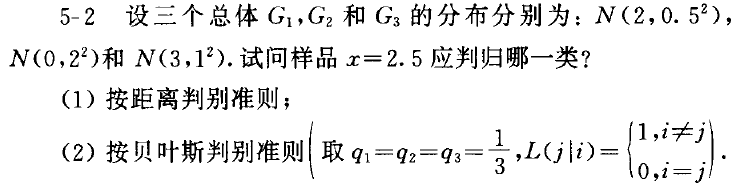
\includegraphics[width=0.8\textwidth]{screenshot001}
\end{figure}
\begin{lstlisting}[language=r]
> d6<-read.csv("E:/4.多元统计分析/图书馆借的书 代码/多元统计分析——基于R(第2版) R-data/eg3.4.csv",header=TRUE)
> table(d6$deaths)

   0    1    2    3    4    5    6 
1833  212   62   28    6    2    1 

> barplot(table(d6$deaths))
\end{lstlisting}
\begin{figure}[H]
	\centering
	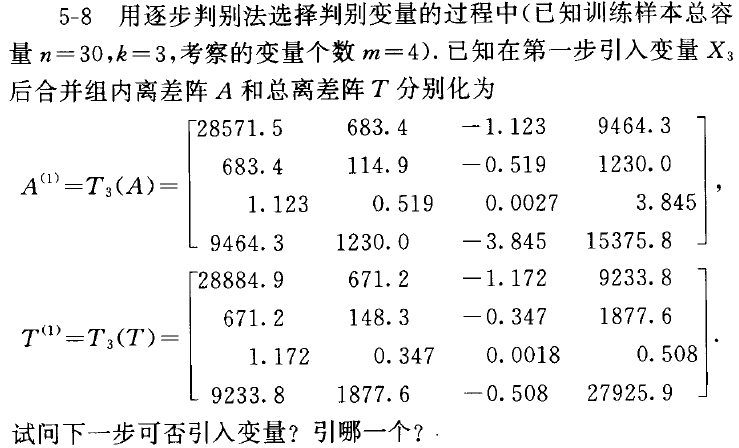
\includegraphics[width=0.6\textwidth]{screenshot002}
\end{figure}

显然,因变量死亡人数(deaths)取值为0的观测值有1833个,属于零膨胀数据,如果不考虑零膨胀问题,直接采用泊松对数线性模型来拟合数据:
\begin{lstlisting}[language=r]
> hiv<-factor(d6$hiv)    #因子化
> fac<-factor(d6$factor)

> a1<-glm(deaths~hiv+fac+age+py,family = poisson(link=log),data=d6)
> summary(a1)

Call:
glm(formula = deaths ~ hiv + fac + age + py, family = poisson(link = log),data = d6)

Deviance Residuals: 
    Min       1Q   Median       3Q      Max  
-1.9151  -0.7494  -0.2083  -0.1597   3.6360  

Coefficients:
             Estimate Std. Error z value Pr(>|z|)    
(Intercept) -7.516867   0.447151 -16.811  < 2e-16 ***
hiv          3.044923   0.206088  14.775  < 2e-16 ***
fac2        -0.634661   0.151608  -4.186 2.84e-05 ***
fac3        -0.388113   0.140312  -2.766  0.00567 ** 
fac4        -0.667857   0.141730  -4.712 2.45e-06 ***
fac5        -0.399791   0.145520  -2.747  0.00601 ** 
age          0.083858   0.014790   5.670 1.43e-08 ***
py           0.022879   0.002544   8.992  < 2e-16 ***
---
Signif. codes:  0 ‘***’ 0.001 ‘**’ 0.01 ‘*’ 0.05 ‘.’ 0.1 ‘ ’ 1

(Dispersion parameter for poisson family taken to be 1)

Null deviance: 1892.8  on 2143  degrees of freedom
Residual deviance: 1291.7  on 2136  degrees of freedom
AIC: 2007.7

Number of Fisher Scoring iterations: 6
\end{lstlisting}
于是可以得到如下泊松对数线性模型:
\[ln(\lambda)=-7.517+\hat{\alpha_i}+\hat{\beta_j}+0.084age+0.023py\]
其中,$ \hat{\alpha_i} $代表hiv=i(i=1,2)对截距的影响,估计结果为
\[\hat{\alpha_1}=0(\mbox{软件默认值})\]
\[\hat{\alpha_2}=3.045\]
$ \hat{\beta_j} $代表factor=j(j=1,2,...,5)对截距的影响,估计结果为
\[\hat{\beta_1}=0(\mbox{软件默认值})\]
\[\hat{\beta_2}=-0.635\]
\[\hat{\beta_3}=-0.388\]
\[\hat{\beta_4}=-0.668\]
\[\hat{\beta_5}=-0.400\]

如果考虑零膨胀问题,则可以采用零膨胀模型来处理:
\begin{lstlisting}[language=r]
> library(pscl)
Classes and Methods for R developed in the
Political Science Computational Laboratory
Desectionment of Political Science
Stanford University
Simon Jackman
hurdle and zeroinfl functions by Achim Zeileis

> a2<-zeroinfl(deaths~hiv+fac+age+py|hiv+age+py,data=d6)
> summary(a2)

Call:
zeroinfl(formula = deaths ~ hiv + fac + age + py | hiv + age + py, data = d6)

Pearson residuals:
     Min       1Q   Median       3Q      Max 
-1.14319 -0.42659 -0.18263 -0.03452 40.55850 

Count model coefficients (poisson with log link):
             Estimate Std. Error z value Pr(>|z|)    
(Intercept) -4.564811   0.730531  -6.249 4.14e-10 ***
hiv          2.143870   0.308923   6.940 3.93e-12 ***
fac2        -0.639624   0.157413  -4.063 4.84e-05 ***
fac3        -0.402610   0.146170  -2.754  0.00588 ** 
fac4        -0.577092   0.147251  -3.919 8.89e-05 ***
fac5        -0.414416   0.151140  -2.742  0.00611 ** 
age         -0.035519   0.024899  -1.427  0.15372    
py           0.028751   0.003557   8.083 6.32e-16 ***

Zero-inflation model coefficients (binomial with logit link):
            Estimate Std. Error z value Pr(>|z|)    
(Intercept)  9.56102    1.80057   5.310 1.10e-07 ***
hiv         -3.25043    0.83818  -3.878 0.000105 ***
age         -0.86075    0.16164  -5.325 1.01e-07 ***
py           0.02750    0.01138   2.416 0.015703 *  
---
Signif. codes:  0 '***' 0.001 '**' 0.01 '*' 0.05 '.' 0.1 ' ' 1 

Number of iterations in BFGS optimization: 43 
Log-likelihood: -928.1 on 12 Df

> AIC(a2)
[1] 1880.295
\end{lstlisting}

从拟合的AIC值可以看出:零膨胀模型的拟合结果显然比一般泊松对数线性模型要好.按照输出结构,零膨胀模型的Logistic回归部分的拟合模型为:
\[\ln(\frac{\pi}{1-\pi})=9.561-3.250hiv-0.861age+0.028py\]
而泊松回归部分的拟合模型为:
\[\ln(\lambda)=-4.565+\hat{\alpha_i}+\hat{\beta_j}-0.036age+0.029py\]
其中,$ \hat{\alpha_i} $代表hiv=i(i=1,2)对截距的影响,估计结果为
\[\hat{\alpha_1}=0(\mbox{软件默认值})\]
\[\hat{\alpha_2}=2.144\]
$ \hat{\beta_j} $代表factor=j(j=1,2,...,5)对截距的影响,估计结果为
\[\hat{\beta_1}=0(\mbox{软件默认值})\]
\[\hat{\beta_2}=-0.640\]
\[\hat{\beta_3}=-0.403\]
\[\hat{\beta_4}=-0.577\]
\[\hat{\beta_5}=-0.414\]

\section{多项分布对数线性模型}
对于计数因变量,在列联表分析中,每个格子中都是各种变量组合的计数,假定有n个格子,如果落入每个格子都有一个概率$ p_i(i=1,..,n) $,那么可以用多项分布来描述这个问题.

如果每个格子计数的均值都随一些自变量的变化而变化,则可以考虑多项分布对数线性模型.

\begin{e}
著名泰坦尼克号的相关数据共有5个变量,2201个观测值,根据给定的数据:

1.以生还概率为关心变量建立合适的模型进行分析;

2.根据模型估计女乘客生还概率比男乘客高多少;

3.根据模型参数估计一等舱乘客生还的概率比三等舱乘客高多少.
\end{e}

\begin{lstlisting}[language=r]
> d7<-read.csv("E:/4.多元统计分析/图书馆借的书 代码/多元统计分析——基于R(第2版) R-data/eg3.5.csv",header=TRUE)
> d7
   Class    Sex   Age Survived Freq
1    1st   Male Child       No    0
2    2nd   Male Child       No    0
3    3rd   Male Child       No   35
4   Crew   Male Child       No    0
5    1st Female Child       No    0
6    2nd Female Child       No    0
7    3rd Female Child       No   17
8   Crew Female Child       No    0
9    1st   Male Adult       No  118
10   2nd   Male Adult       No  154
11   3rd   Male Adult       No  387
12  Crew   Male Adult       No  670
13   1st Female Adult       No    4
14   2nd Female Adult       No   13
15   3rd Female Adult       No   89
16  Crew Female Adult       No    3
17   1st   Male Child      Yes    5
18   2nd   Male Child      Yes   11
19   3rd   Male Child      Yes   13
20  Crew   Male Child      Yes    0
21   1st Female Child      Yes    1
22   2nd Female Child      Yes   13
23   3rd Female Child      Yes   14
24  Crew Female Child      Yes    0
25   1st   Male Adult      Yes   57
26   2nd   Male Adult      Yes   14
27   3rd   Male Adult      Yes   75
28  Crew   Male Adult      Yes  192
29   1st Female Adult      Yes  140
30   2nd Female Adult      Yes   80
31   3rd Female Adult      Yes   76
32  Crew Female Adult      Yes   20
\end{lstlisting}

显然这个列联表是4x2x2x2维的,一共有32个格子,由于都是分类变量,所以相对应得多项分布对数线性模型为:
\[\ln\mu_{ijk}=\ln n_{ijk}+\mu+Class_i+Sex_j+Age_k, i=1,2,3,4; j=1,2; k=1,2\]
其中$ \mu_{ijk} $表示格子(i,j,k)里生还的平均人数,$ n_{ijk} $表示格子(i,j,k)里总人数.

若以生还概率为关心变量,等价地建立以下多项分布对数线性模型:
\[\ln\frac{\mu_{ijk}}{n_{ijk}}=\mu+Class_i+Sex_j+Age_k, i=1,2,3,4; j=1,2; k=1,2\]
即生还概率为:
\[\frac{\mu_{ijk}}{n_{ijk}}=\exp\left\lbrace \mu+Class_i+Sex_j+Age_k\right\rbrace , i=1,2,3,4; j=1,2; k=1,2\]

\begin{lstlisting}[language=r]
> library(MASS)
> w<-d7[d7$Survived=="Yes",]  #统计生还人数
> w$n<-d7[1:16,5]+d7[17:32,5]  #构建包含总人数n的数据w
> w<-w[w$n!=0,]   #去掉n为0的数据
> w.fit<-glm(Freq~Class+Sex+Age,family = poisson,data=w,offset=log(n))
> summary(w.fit)

Call:
glm(formula = Freq ~ Class + Sex + Age, family = poisson, data = w, 
offset = log(n))

Deviance Residuals: 
    Min       1Q   Median       3Q      Max  
-4.0906  -0.4338   0.1433   0.9919   3.0362  

Coefficients:
             Estimate Std. Error z value Pr(>|z|)    
(Intercept)  0.008821   0.074509   0.118 0.905757    
Class2nd    -0.376492   0.117564  -3.202 0.001363 ** 
Class3rd    -0.764527   0.106891  -7.152 8.53e-13 ***
ClassCrew   -0.303959   0.113666  -2.674 0.007492 ** 
SexMale     -1.191743   0.089211 -13.359  < 2e-16 ***
AgeChild     0.480281   0.145603   3.299 0.000972 ***
---
Signif. codes:  0 ‘***’ 0.001 ‘**’ 0.01 ‘*’ 0.05 ‘.’ 0.1 ‘ ’ 1

(Dispersion parameter for poisson family taken to be 1)

Null deviance: 348.387  on 13  degrees of freedom
Residual deviance:  38.881  on  8  degrees of freedom
AIC: 121.57

Number of Fisher Scoring iterations: 4
\end{lstlisting}

为了查看模型拟合效果,我们把实际数据的生还人数和模型拟合的生还人数进行对比:
\begin{lstlisting}[language=r]
> plot(w$Freq,w.fit$fitted.values,xlab="实际生还人数",ylab="模型拟合生还人数")
> lines(c(0,200),c(0,200))
\end{lstlisting}
\begin{figure}[H]
	\centering
	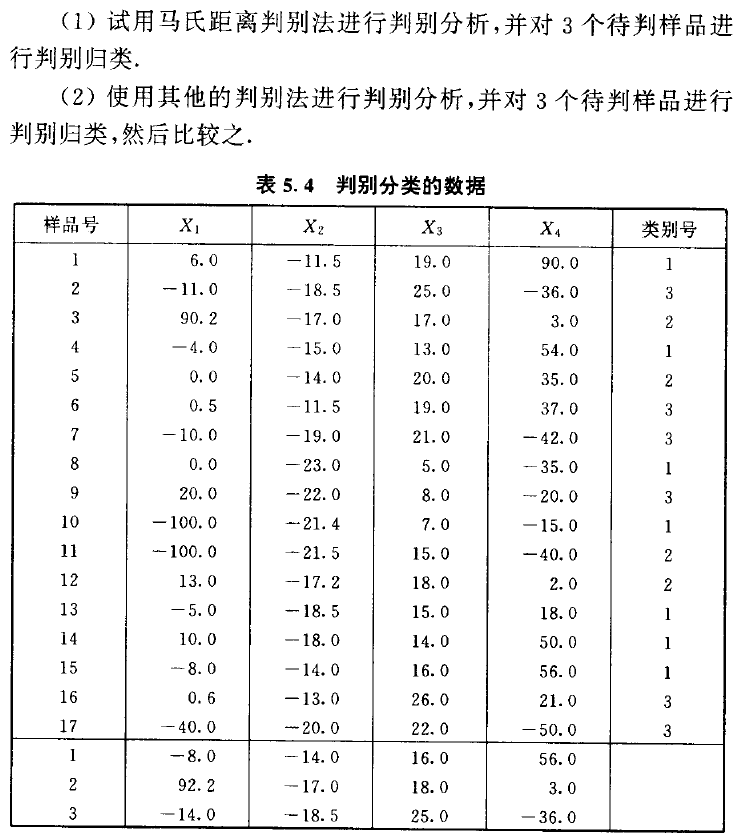
\includegraphics[width=0.6\textwidth]{screenshot004}
\end{figure}
图形说明模型拟合效果比较好.

第二问和第三问根据模型意义和参数估计结果可以计算,在其他条件相同时:
\[\frac{\mbox{女乘客生还概率}}{\mbox{男乘客生还概率}}=\frac{\exp\left\lbrace 0\right\rbrace }{\exp\left\lbrace -1.1917\right\rbrace}=3.2927\]
\[\frac{\mbox{一等舱乘客生还概率}}{\mbox{三等舱乘客生还概率}}=\frac{\exp\left\lbrace 0\right\rbrace }{\exp\left\lbrace -0.7645\right\rbrace}=2.1479\]

\chapter{回归分析}
\section{经典回归模型的基本要素}
\begin{figure}[H]
	\centering
	\includegraphics[width=0.8\textwidth]{screenshot105}
\end{figure}
\begin{figure}[H]
	\centering
	\includegraphics[width=0.8\textwidth]{screenshot106}
\end{figure}
\begin{lstlisting}[language=r]
	
\end{lstlisting}
\begin{lstlisting}[language=r]
	
\end{lstlisting}
\begin{lstlisting}[language=r]
	
\end{lstlisting}
\chapter{聚类分析}
\section{相似性度量}
\begin{definition}
\textbf{欧氏距离}:\[d(x,y)=\sqrt{\sum_{i=1}^{p}(x_i-y_i)^2}\]
\end{definition}
\begin{definition}
	\textbf{绝对距离}:\[d(x,y)=\sum_{i=1}^{p}|x_i-y_i|\]
\end{definition}
\begin{definition}
	\textbf{Chebyshev距离}:\[d(x,y)=max_i|x_i-y_i|\]
\end{definition}
\begin{definition}
	\textbf{Minkowski距离}:\[d(x,y)=(\sum_{i=1}^{p}|x_i-y_i|^k)^{\frac{1}{k}}\]
\end{definition}
\begin{definition}
	\textbf{Mahalanobis距离}:\[d(x,y)=\sqrt{(x-y)^TS^{-1}(x-y)}\]
\end{definition}
\begin{definition}
	\textbf{Lance距离}:\[d(x,y)=\sum_{i=1}^{p}\frac{|x_i-y_i|}{x_i+y_i}\]
\end{definition}

\begin{figure}[H]
	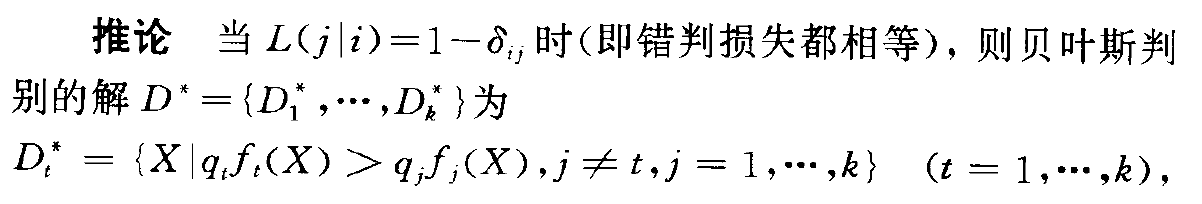
\includegraphics[width=0.6\textwidth]{screenshot007}
\end{figure}
\begin{figure}[H]
	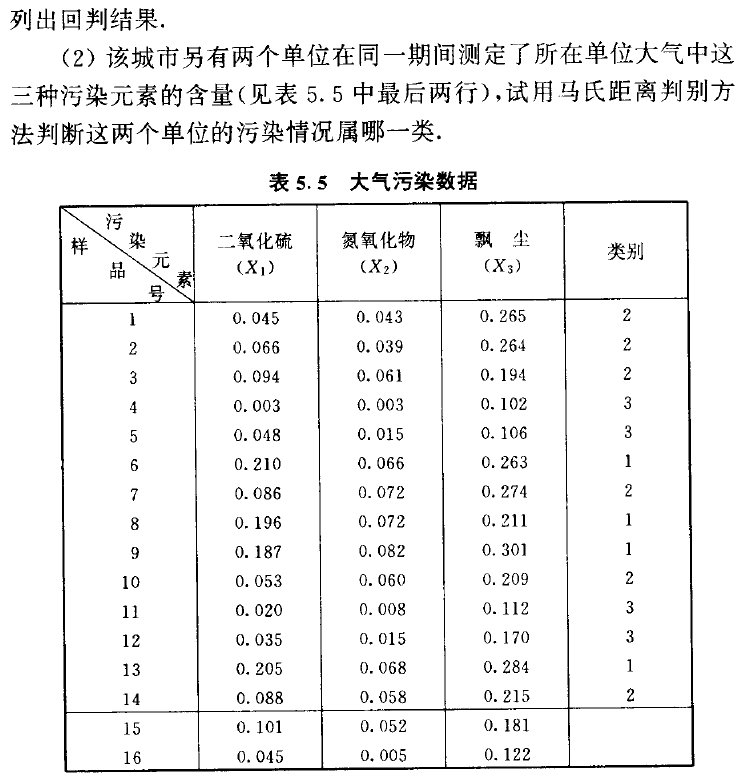
\includegraphics[width=0.6\textwidth]{screenshot006}
\end{figure}

\begin{lstlisting}[language=r]
#对X的列向量作不减样本均值的标准化
> Y<-scale(X, center=F, scale=T)/sqrt(nrow(X)-1)

#可计算出X的列向量间的夹角余弦
> C<-t(Y)%*%Y

#计算X的列向量间的相关系数矩阵
> R<-cor(X)
\end{lstlisting}
程序中center是逻辑变量,真表示对数据做中心变换; scale也是逻辑变量,真表示对数据做标准化变换.
\section{系统聚类法}
\textbf{Q型聚类情形}:
\begin{enumerate}
	\item 最小距离法
	\item 最大距离法
	\item 中间距离法
	\item 重心距离法
	\item 类平均距离法
	\item Ward法
\end{enumerate}

\textbf{R型聚类情形}:\[R_{st}={max_{i\in G_s, j\in G_t}|r_{ij}|}\]
\begin{figure}[H]
	\includegraphics[width=0.5\textwidth]{screenshot028}
	\label{fig:screenshot028}
\end{figure}
\begin{figure}[H]
	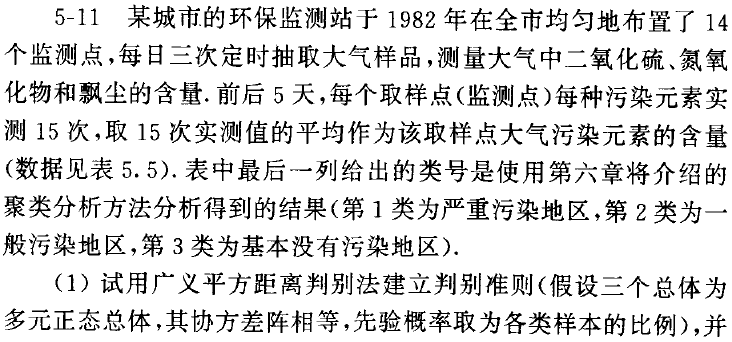
\includegraphics[width=0.4\textwidth]{screenshot005}
\end{figure}
\begin{e}
	为比较10种红葡萄酒的质量,由5位品酒师对每种酒的6项指标进行打分,最低1,最高10,用系统聚类法的最小距离法和最大距离法对十种酒进行聚类.
\end{e}
\begin{lstlisting}[language=r]
> eg4.1<-read.csv("E:/4.多元统计分析/图书馆借的书 代码/多元统计分析——基于R(第2版) R-data/eg4.1.csv")
> d<-dist(eg4.1,method="euclidean",diag=T,upper=F,p=2) #欧氏距离算相似阵d
> d=round(d,3);
> d
       1     2     3     4     5     6     7     8     9    10
1  0.000                                                      
2  4.881 0.000                                                
3  0.580 4.944 0.000                                          
4  0.872 5.073 0.528 0.000                                    
5  5.138 1.113 5.097 5.260 0.000                              
6  7.434 2.720 7.436 7.601 2.461 0.000                        
7  9.129 4.364 9.113 9.260 4.025 1.860 0.000                  
8  9.261 4.558 9.222 9.371 4.140 1.985 0.544 0.000            
9  4.875 1.015 4.835 4.987 0.569 2.659 4.319 4.421 0.000      
10 7.027 2.343 7.023 7.187 2.040 0.484 2.214 2.315 2.262 0.000

#method为距离计算方法,包括"euclidean"欧氏距离, "manhattan"绝对距离,
#"maximum"切氏距离, "minkowski"明氏距离, "canberra"兰氏距离等;
#diag为是否包括对角元素,upper为是否需要上三角元素

> HC<-hclust(d,method="single") #采用最小距离法(single)聚类
> plot(HC,hang=-1)  #当hang取负值时,从底部对齐开始绘制聚类树状图

#method为系统聚类方法,包括"single"最小距离法,"complete"最大距离法,
#"average"类平均法,"median"中间距离法,"centroid"重心法,"ward"Ward法 等
\end{lstlisting}
\begin{figure}[H]
	\centering
	\includegraphics[width=0.9\textwidth]{screenshot029}
	\label{fig:screenshot029}
\end{figure}

\begin{lstlisting}[language=r]
> abline(h=4) ; abline(h=1.95)  
#在图4.2中分别画合并距离为4和1.95的水平线帮助准确分类
\end{lstlisting}
\begin{figure}[H]
	\centering
	\includegraphics[width=0.7\textwidth]{screenshot030}
	\label{fig:screenshot030}
\end{figure}

\begin{lstlisting}[language=r]
> x11() #另开一个绘图窗口
> plot(HC) #绘制最小距离法聚类树状图,但底部对不齐. 两图可以相互对比
\end{lstlisting}
\begin{figure}[H]
	\centering
	\includegraphics[width=0.7\textwidth]{screenshot031}
	\label{fig:screenshot031}
\end{figure}

\begin{lstlisting}[language=r]
> HC1<-hclust(d,method="complete") #采用最大距离法(complete)聚类
> plot(HC1,hang=-1)#绘制最大距离法聚类树状图
> rect.hclust(HC1,k=3,border="red") #用矩形框出3个分类的结果
> rect.hclust(HC1,k=2,border="blue")
\end{lstlisting}
\begin{figure}[H]
	\centering
	\includegraphics[width=0.7\textwidth]{screenshot032}
	\label{fig:screenshot032}
\end{figure}

对hclust函数聚类的结果进行剪枝,即选择输出指定分类个数的聚类结果
\begin{lstlisting}[language=r]
> cutree(HC1,k=3)
[1] 1 2 1 1 2 3 3 3 2 3
\end{lstlisting}
输出结果表明10种酒可以分为三类,他们对应于1,2和3所在的位置,分别为(1,3,4),(2,5,9),(6,7,8,10)

\section{K-means聚类法}
\begin{e}
2015年全国31个省,市,自治区(不含港澳台)居民消费支出的8项主要指标数据,采用k均值聚类法进行聚类分析,k分别取4和5.
\end{e}
\begin{lstlisting}[language=r]
> eg42<-read.csv("E:/4.多元统计分析/图书馆借的书 代码/多元统计分析——基于R(第2版) R-data/eg4.2.csv")
> head(eg42)
        X     x1     x2      x3     x4     x5     x6     x7    x8
1    北京 7584.2 2425.7 10350.2 2098.3 4489.6 3634.6 2228.6 991.4
2    天津 7709.9 1949.4  5237.5 1514.0 3185.9 2096.0 1757.1 712.6
3    河北 3515.5 1055.3  2995.8  832.2 1807.6 1338.6 1192.0 293.6
4    山西 3089.4 1146.7  2297.4  672.5 1501.4 1628.0 1102.0 291.5
5  内蒙古 4919.8 1759.7  2918.9 1030.9 2569.0 2067.1 1384.3 528.9
6    辽宁 4858.0 1561.6  3471.6 1028.7 2282.0 1973.3 1522.4 502.2

> d42<-eg42[,-1]  #去掉第一列地名
> rownames(d42) <- eg42[,1]   #用地名作行名
> head(d42)
x1     x2      x3     x4     x5     x6     x7    x8
北京   7584.2 2425.7 10350.2 2098.3 4489.6 3634.6 2228.6 991.4
天津   7709.9 1949.4  5237.5 1514.0 3185.9 2096.0 1757.1 712.6
河北   3515.5 1055.3  2995.8  832.2 1807.6 1338.6 1192.0 293.6
山西   3089.4 1146.7  2297.4  672.5 1501.4 1628.0 1102.0 291.5
内蒙古 4919.8 1759.7  2918.9 1030.9 2569.0 2067.1 1384.3 528.9
辽宁   4858.0 1561.6  3471.6 1028.7 2282.0 1973.3 1522.4 502.2

> KM <- kmeans(d42,4,nstart = 20,algorithm = "Hartigan-Wong") #初始随机集合的个数为20,算法为"Hartigan-Wong"(默认)
> KM
K-means clustering with 4 clusters of sizes 15, 5, 2, 9

Cluster means:
x1       x2        x3        x4       x5       x6       x7       x8
1 3682.120 1008.667  2409.193  730.2867 1578.887 1362.813 1053.360 278.8733
2 6859.680 1449.800  5013.720 1240.8600 3091.480 2170.020 1320.880 585.7200
3 8427.850 2024.200 10828.850 1791.4500 4348.050 3676.350 2248.450 947.8500
4 4788.289 1177.544  2834.878  914.3667 1898.144 1618.178 1160.667 355.4667

Clustering vector:
北京  天津  河北  山西  内蒙古    辽宁    吉林  黑龙江    上海    江苏 
3     2     1     1     4       4       1       1       3       2 
浙江  安徽  福建  江西    山东    河南    湖北    湖南    广东    广西 
2     4     2     1     4       1       4       4       2       1 
海南  重庆  四川  贵州    云南    西藏    陕西    甘肃    青海    宁夏 
4     4     4     1     1       1       1       1       1       1 
新疆 
1 

Within cluster sum of squares by cluster:
[1] 9408235 6090537 2440561 5448008
(between_SS / total_SS =  91.3 %)  #类间平方和在总平方和中的占比,越大越好

Available components:

[1] "cluster"      "centers"      "totss"        "withinss"     "tot.withinss"
[6] "betweenss"    "size"         "iter"         "ifault"      

> sort(KM$cluster)  #对分类结果进行排序并查看分类结果
河北    山西    吉林  黑龙江    江西    河南    广西    贵州 
1       1       1       1       1       1       1       1 
云南    西藏    陕西    甘肃    青海    宁夏    新疆    天津 
1       1       1       1       1       1       1       2 
江苏    浙江    福建    广东    北京    上海  内蒙古    辽宁 
2       2       2       2       3       3       4       4 
安徽    山东    湖北    湖南    海南    重庆    四川 
4       4       4       4       4       4       4 
\end{lstlisting}

\begin{e}
对305名女学生测量8个体型变量,相应的相关关系矩阵$ R=(r_{ij}) $.若定义变量之间的距离$ d_{ij}=1-r_{ij} $,可得到变量间的距离矩阵$ d=(d_{ij}) $.据此用系统聚类法和k均值聚类法对8个体型变量进行聚类,并对比合并距离分别为0.8和0.6的系统聚类结果与k分别取2和3的k均值聚类结果.
\end{e}
\begin{lstlisting}[language=r]
> eg43<-read.csv("E:/4.多元统计分析/图书馆借的书 代码/多元统计分析——基于R(第2版) R-data/eg4.3.csv")
> View(eg43)
> eg43
        X  身高 手臂长 上肢长 下肢长  体重  颈围  胸围  胸宽
1   身高 1.000  0.846  0.805  0.859 0.473 0.398 0.301 0.382
2 手臂长 0.846  1.000  0.881  0.826 0.376 0.326 0.277 0.415
3 上肢长 0.805  0.881  1.000  0.801 0.380 0.319 0.237 0.345
4 下肢长 0.859  0.826  0.801  1.000 0.436 0.329 0.327 0.365
5   体重 0.473  0.376  0.380  0.436 1.000 0.762 0.730 0.629
6   颈围 0.398  0.326  0.319  0.329 0.762 1.000 0.583 0.577
7   胸围 0.301  0.277  0.237  0.327 0.730 0.583 1.000 0.539
8   胸宽 0.382  0.277  0.345  0.365 0.629 0.577 0.539 1.000

> d43<-eg43[,-1]
> rownames(d43) <- eg43[,1]
> d=dist(1-d43)  #将相关系数阵转换成距离阵
> d
          身高    手臂长    上肢长    下肢长      体重      颈围
手臂长 0.2656219                                                  
上肢长 0.3177955 0.1928549                                        
下肢长 0.2174235 0.2751908 0.3112539                              
体重   1.2302268 1.3274347 1.3368725 1.2587784                    
颈围   1.3089591 1.3931924 1.3940746 1.3461363 0.4011184          
胸围   1.4253189 1.4876024 1.4958870 1.4205446 0.5075983 0.6072759
胸宽   1.2869600 1.3325618 1.3459792 1.2988506 0.6085524 0.6181521

        胸围
手臂长          
上肢长          
下肢长          
体重            
颈围            
胸围            
胸宽   0.6744983
> HC <- hclust(d,method = "average")   #采用类平均法作系统聚类
> plot(HC,hang=-1) #从底部对齐绘制聚类树状图
> abline(h=0.8)
> abline(h=0.6)
\end{lstlisting}
\begin{figure}[H]
	\centering
	\includegraphics[width=0.9\textwidth]{screenshot008}
\end{figure}

用k均值聚类法:
\begin{lstlisting}[language=r]
> KM2 <- kmeans(d,2,nstart = 5,algorithm = "Hartigan-Wong")
> sort(KM2$cluster)
体重   颈围   胸围   胸宽   身高 手臂长 上肢长 下肢长 
1      1      1      1      2      2      2      2 

> KM3 <- kmeans(d,3,nstart = 5,algorithm = "Hartigan-Wong")
> sort(KM3$cluster)
身高 手臂长 上肢长 下肢长   胸宽   体重   颈围   胸围 
1      1      1      1      2      3      3      3 
\end{lstlisting}

\section{EM聚类法}
除了系统聚类hclust()和k均值聚类kmeans(),其他的聚类函数如\textbf{K-中心点聚类pam()}(clust包),进行\textbf{密度聚类dbscan()}(fpc包),进行\textbf{期望最大化聚类EM聚类Mclust()}(mclust包)

函数Mclust()使用格式: \textbf{Mclust(data,G,modelNames,prior,control,...)},其中G为预设类别数,默认值1-9,由软件根据BIC值选择最优值,modelNames用于设定模型类别,也由函数自动选取最优值.
\begin{figure}[H]
	\centering
	\includegraphics[width=\textwidth]{screenshot013}
\end{figure}

\begin{e}
R内置数据中有一个由地质学将于1978.8至1979.8在美国黄石公园旅游景点oldfaithful泉记录的间歇喷泉喷发数据.faithful数据集由272行2列:泉水喷发持续时间eruptions,喷发间隔时间waiting,时间单位均为分钟.以下用两种方法进行EM聚类.
\end{e}

\begin{lstlisting}[language=r]
> library(mclust)
    __  ___________    __  _____________
   /  |/  / ____/ /   / / / / ___/_  __/
  / /|_/ / /   / /   / / / /\__ \ / /   
 / /  / / /___/ /___/ /_/ /___/ // /    
/_/  /_/\____/_____/\____//____//_/    version 5.4.7
Type 'citation("mclust")' for citing this R package in publications.

> EM1 <- Mclust(faithful)
fitting ...
|=============================================================| 100%

> summary(EM1,parameters = T)
---------------------------------------------------- 
Gaussian finite mixture model fitted by EM algorithm 
---------------------------------------------------- 

Mclust EEE (ellipsoidal, equal volume, shape and orientation) model
with 3 components: 

log-likelihood   n df       BIC       ICL
     -1126.326 272 11 -2314.316 -2357.824

Clustering table:
1   2   3 
40  97 135 

Mixing probabilities:
1         2         3 
0.1656784 0.3563696 0.4779520 

Means:
               [,1]      [,2]      [,3]
eruptions  3.793066  2.037596  4.463245
waiting   77.521051 54.491158 80.833439

Variances:
[,,1]
           eruptions    waiting
eruptions 0.07825448  0.4801979
waiting   0.48019785 33.7671464
[,,2]
           eruptions    waiting
eruptions 0.07825448  0.4801979
waiting   0.48019785 33.7671464
[,,3]
           eruptions    waiting
eruptions 0.07825448  0.4801979
waiting   0.48019785 33.7671464

> plot(EM1,what = "classification")
\end{lstlisting}
\begin{figure}[H]
	\centering
	\includegraphics[width=0.8\textwidth]{screenshot009}
\end{figure}
从程序输出结果和图易见,全部272个原始数据被聚为三类.

另一种聚类方法为:首先在faithful数据分布范围内随机生成600个均匀分布随机数,将它们与原来的的faithful数据混合得到872个的混合样本数据,再用Mclust()对混合数据作EM聚类分析.
\begin{lstlisting}[language=r]
#设定均匀分布噪声数据个数
> nNoise <- 600  
#设置随机数种子
> set.seed(8)
#在faithful数据分布范围内生成nNoise=600行,2列的均匀分布噪声数据
> Noise <- apply(faithful,2,function(x)runif(nNoise,min=min(x)-0.1,max = max(x)+0.1))
#按行合并faithful和Noise,得到872个混合数据样本
> data <- rbind(faithful,Noise)
#绘制三点图
> plot(faithful)
\end{lstlisting}
\begin{figure}[H]
	\centering
	\includegraphics[width=0.8\textwidth]{screenshot011}
\end{figure}

\begin{lstlisting}[language=r]
> library(mclust)
> NoiseInit <- sample(c(TRUE,FALSE),size=nrow(faithful)+nNoise,replace=TRUE,prob = c(3,1)/4)
> EM2 <- Mclust(data,initialization = list(noise=NoiseInit))
fitting ...
|=============================================================| 100%
> summary(EM2,parameters = T)
---------------------------------------------------- 
Gaussian finite mixture model fitted by EM algorithm 
---------------------------------------------------- 

Mclust VEI (diagonal, equal shape) model with 2 components and a noise
term: 

log-likelihood   n df       BIC       ICL
-4506.676 872 10 -9081.059 -9437.114

Clustering table:
1   2   0 
158  88 626 

Mixing probabilities:
1          2          0 
0.17092862 0.09520339 0.73386799 

Means:
              [,1]      [,2]
eruptions  4.31705  1.986842
waiting   79.53881 52.678829

Variances:
[,,1]
          eruptions  waiting
eruptions  0.110578  0.00000
waiting    0.000000 38.44398
[,,2]
           eruptions  waiting
eruptions 0.04896398  0.00000
waiting   0.00000000 17.02301

Hypervolume of noise component:
195.9458 
> plot(EM2,what = "classification")
\end{lstlisting}
\begin{figure}[H]
	\centering
	\includegraphics[width=0.9\textwidth]{screenshot012}
\end{figure}
从程序的输出结果可知,全部872个原始数据被聚为2类,样本大小分别为156(蓝圆点),87(红空心方块),其余629个被视为噪声点.

对混合样本的EM聚类基本没有收到均匀分布噪声的影响.在样本数据量较小的时候,适当加入一些均匀分布数据点有时可以改进聚类效果.
\section{类的个数}
\begin{figure}[H]
	\includegraphics[width=0.7\textwidth]{screenshot033}
	\label{fig:screenshot033}
\end{figure}

\begin{lstlisting}[language=r]
> library(NbClust)
> eg4.1.sl<-scale(eg4.1)
> eg4.1.sl.nc<-NbClust(eg4.1.sl,distance = "euclidean",min.nc = 2,max.nc = 5,method = "average")
*** : The Hubert index is a graphical method of determining the number of clusters. In the plot of Hubert index, we seek a significant knee that corresponds to a significant increase of the value of the measure i.e the significant peak in Hubert index second differences plot. 

*** : The D index is a graphical method of determining the number of clusters. In the plot of D index, we seek a significant knee (the significant peak in D index second differences plot) that corresponds to a significant increase of the value of the measure. 

******************************************************************* 
* Among all indices:                                                
* 5 proposed 2 as the best number of clusters 
* 5 proposed 3 as the best number of clusters 
* 7 proposed 4 as the best number of clusters 
* 7 proposed 5 as the best number of clusters 

***** Conclusion *****                            

* According to the majority rule, the best number of clusters is  4 

******************************************************************* 
\end{lstlisting}
\begin{figure}[H]
	\centering
	\includegraphics[width=0.7\textwidth]{screenshot034}
	\label{fig:screenshot034}
\end{figure}

\begin{lstlisting}[language=r]
> table(eg4.1.sl.nc$Best.nc[1,])

0 2 3 4 5 
2 5 5 7 7 
\end{lstlisting}

\chapter{判别分析}
判别分析是在已知样品分类的前提下,将给定的新样品按照某种分类准则判入某个类中.
\section{距离判别}
在判别分析中,马氏距离更常用,因为欧氏距离对每一样品等同对待,将样品x的各分量视作互不相关,而马氏距离考虑了样品数据之间的依存关系.
\subsection{两个总体的距离判别}
\begin{figure}[H]
	\centering
	\includegraphics[width=0.6\textwidth]{screenshot014}
\end{figure}
\begin{figure}[H]
	\centering
	\includegraphics[width=0.6\textwidth]{screenshot015}
\end{figure}
\begin{figure}[H]
	\centering
	\includegraphics[width=0.8\textwidth]{screenshot016}
\end{figure}

两总体的距离判别函数:
\begin{lstlisting}[language=r]
 DDA2<-function (TrnG1, TrnG2, TstG = NULL, var.equal = FALSE){
	if (is.null(TstG) == TRUE) TstG<-rbind(TrnG1,TrnG2)
	if (is.vector(TstG) == TRUE)  TstG<-t(as.matrix(TstG)) else if (is.matrix(TstG) != TRUE)
	TstG<-as.matrix(TstG)
	if (is.matrix(TrnG1) != TRUE) TrnG1<-as.matrix(TrnG1)
	if (is.matrix(TrnG2) != TRUE) TrnG2<-as.matrix(TrnG2); 
	nx<-nrow(TstG)
	blong<-matrix(rep(0, nx), nrow=1, byrow=TRUE, dimnames=list("blong", 1:nx))
	mu1<-colMeans(TrnG1); mu2<-colMeans(TrnG2) 
	if (var.equal == TRUE  || var.equal == T){
		S<-var(rbind(TrnG1,TrnG2))
		w<-mahalanobis(TstG, mu2, S)-mahalanobis(TstG, mu1, S)
	} else{
		S1<-var(TrnG1); S2<-var(TrnG2)
		w<-mahalanobis(TstG, mu2, S2)-mahalanobis(TstG, mu1, S1)
	}
	for (i in 1:nx){if (w[i]>0) blong[i]<-1 else blong[i]<-2}; blong
}

\end{lstlisting}
\begin{figure}[H]
	\centering
	\includegraphics[width=0.8\textwidth]{screenshot018}
\end{figure}

多总体判别函数:
\begin{lstlisting}[language=r]
DDAM<-function (TrnX, TrnG, TstX = NULL, var.equal = FALSE){
	if ( is.factor(TrnG) == FALSE){
		mx<-nrow(TrnX); mg<-nrow(TrnG)
		TrnX<-rbind(TrnX, TrnG)
		TrnG<-factor(rep(1:2, c(mx, mg)))
	}
	if (is.null(TstX) == TRUE) TstX<-TrnX
	if (is.vector(TstX) == TRUE)  TstX<-t(as.matrix(TstX))
	else if (is.matrix(TstX) != TRUE)
	TstX<-as.matrix(TstX)
	if (is.matrix(TrnX) != TRUE) TrnX<-as.matrix(TrnX)
	nx<-nrow(TstX)
	blong<-matrix(rep(0, nx), nrow=1, dimnames=list("blong", 1:nx))
	g<-length(levels(TrnG))
	mu<-matrix(0, nrow=g, ncol=ncol(TrnX))
	for (i in 1:g)
	mu[i,]<-colMeans(TrnX[TrnG==i,]) 
	D<-matrix(0, nrow=g, ncol=nx)
	if (var.equal == TRUE  || var.equal == T){
		for (i in 1:g)
		D[i,]<- mahalanobis(TstX, mu[i,], var(TrnX))
	}
	else{
		for (i in 1:g)
		D[i,]<- mahalanobis(TstX, mu[i,], var(TrnX[TrnG==i,]))
	}
	for (j in 1:nx){
		dmin<-Inf
		for (i in 1:g)
		if (D[i,j]<dmin){
			dmin<-D[i,j]; blong[j]<-i
		}
	}
	blong
}

\end{lstlisting}
\begin{figure}[H]
	\centering
	\includegraphics[width=0.8\textwidth]{screenshot017}
\end{figure}
\section{Fisher判别}
\begin{figure}[H]
	\centering
	\includegraphics[width=0.6\textwidth]{screenshot044}
\end{figure}
\begin{figure}[H]
	\centering
	\includegraphics[width=0.6\textwidth]{screenshot045}
\end{figure}
\begin{e}
	对iris作Fisher判别.
\end{e}
\begin{lstlisting}[language=r]
> data("iris")
> force(iris)
Sepal.Length Sepal.Width Petal.Length Petal.Width    Species
1            5.1         3.5          1.4         0.2     setosa
2            4.9         3.0          1.4         0.2     setosa
3            4.7         3.2          1.3         0.2     setosa
4            4.6         3.1          1.5         0.2     setosa
......
147          6.3         2.5          5.0         1.9  virginica
148          6.5         3.0          5.2         2.0  virginica
149          6.2         3.4          5.4         2.3  virginica
150          5.9         3.0          5.1         1.8  virginica
> attach(iris)  #把数据框变量名读入内存以使用
> library(MASS)  #加载MASS包使用lda
> ld <- lda(Species~Sepal.Length+Sepal.Width+Petal.Length+Petal.Width)
> ld
Call:
lda(Species ~ Sepal.Length + Sepal.Width + Petal.Length + Petal.Width)  #公式

Prior probabilities of groups:   #先验概率
   setosa versicolor  virginica 
0.3333333  0.3333333  0.3333333 

Group means:  #各组均值向量
           Sepal.Length Sepal.Width Petal.Length Petal.Width
setosa            5.006       3.428        1.462       0.246
versicolor        5.936       2.770        4.260       1.326
virginica         6.588       2.974        5.552       2.026

Coefficients of linear discriminants:  #第一及第二线性判别函数的系数
                    LD1         LD2
Sepal.Length  0.8293776  0.02410215
Sepal.Width   1.5344731  2.16452123
Petal.Length -2.2012117 -0.93192121
Petal.Width  -2.8104603  2.83918785

Proportion of trace:  #两个判别式的贡献
   LD1    LD2 
0.9912 0.0088 
\end{lstlisting}

predict()可以对原始数据进行回判分类,从而将lda()的输出结果与原始数据真正的分类进行对比,考察大小.
\begin{lstlisting}[language=r]
> z=predict(ld)
> newG=z$class
> cbind(Species,newG,z$posterior)
    Species newG       setosa   versicolor    virginica
1         1    1 1.000000e+00 3.896358e-22 2.611168e-42
2         1    1 1.000000e+00 7.217970e-18 5.042143e-37
3         1    1 1.000000e+00 1.463849e-19 4.675932e-39
4         1    1 1.000000e+00 1.268536e-16 3.566610e-35
5         1    1 1.000000e+00 1.637387e-22 1.082605e-42
......
147       3    3 4.616611e-36 5.898784e-03 9.941012e-01
148       3    3 5.548962e-35 3.145874e-03 9.968541e-01
149       3    3 1.613687e-40 1.257468e-05 9.999874e-01
150       3    3 2.858012e-33 1.754229e-02 9.824577e-01

> tab <- table(newG,Species)
> tab
             Species
newG         setosa versicolor virginica
setosa         50          0         0
versicolor      0         48         1
virginica       0          2        49
\end{lstlisting}
\begin{lstlisting}[language=r]
> newdata=data.frame(Sepal.Length =c(5.1,5.9,6.6), Sepal.Width =c(3.5,2.8,2.9),Petal.Length =c(1.5,4.3,5.6), Petal.Width =c(0.25,1.3,2.1))
> predict(ld,newdata)
$class
[1] setosa     versicolor virginica 
Levels: setosa versicolor virginica

$posterior
        setosa   versicolor    virginica
1 1.000000e+00 1.117074e-20 3.314219e-40
2 2.963609e-20 9.998273e-01 1.727265e-04
3 4.169387e-42 3.505610e-05 9.999649e-01

$x
        LD1        LD2
1  7.701156  0.3491879
2 -1.823849 -0.7749274
3 -6.199781  0.5182489
\end{lstlisting}
\section{Bayes判别}
在各总体的概率分布及先验概率已知的前提下,分别计算待判对象属于各总体的后验概率,并以最大后验概率对应的总体来作为待判对象的所属总体。
\begin{figure}[H]
	\centering
	\includegraphics[width=0.6\textwidth]{screenshot046}
\end{figure}
\begin{figure}[H]
	\centering
	\includegraphics[width=0.6\textwidth]{screenshot047}
\end{figure}
\begin{figure}[H]
	\centering
	\includegraphics[width=0.6\textwidth]{screenshot048}
\end{figure}
\begin{figure}[H]
	\centering
	\includegraphics[width=0.6\textwidth]{screenshot049}
\end{figure}
\begin{figure}[H]
	\centering
	\includegraphics[width=0.6\textwidth]{screenshot050}
\end{figure}
\begin{figure}[H]
	\centering
	\includegraphics[width=0.6\textwidth]{screenshot051}
\end{figure}
\begin{figure}[H]
	\centering
	\includegraphics[width=\textwidth]{screenshot052}
\end{figure}

\begin{lstlisting}[language=r]
> library(klaR)
> data("iris")
> m <- NaiveBayes(Species~.,data=iris)
> m
$apriori
grouping
setosa versicolor  virginica 
0.3333333  0.3333333  0.3333333 

$tables
$tables$Sepal.Length
            [,1]      [,2]
setosa     5.006 0.3524897
versicolor 5.936 0.5161711
virginica  6.588 0.6358796

$tables$Sepal.Width
            [,1]      [,2]
setosa     3.428 0.3790644
versicolor 2.770 0.3137983
virginica  2.974 0.3224966

$tables$Petal.Length
            [,1]      [,2]
setosa     1.462 0.1736640
versicolor 4.260 0.4699110
virginica  5.552 0.5518947

$tables$Petal.Width
            [,1]      [,2]
setosa     0.246 0.1053856
versicolor 1.326 0.1977527
virginica  2.026 0.2746501


$levels
[1] "setosa"     "versicolor" "virginica" 

$call
NaiveBayes.default(x = X, grouping = Y)

$x
    Sepal.Length Sepal.Width Petal.Length Petal.Width
1            5.1         3.5          1.4         0.2
2            4.9         3.0          1.4         0.2
3            4.7         3.2          1.3         0.2
4            4.6         3.1          1.5         0.2
5            5.0         3.6          1.4         0.2
......
146          6.7         3.0          5.2         2.3
147          6.3         2.5          5.0         1.9
148          6.5         3.0          5.2         2.0
149          6.2         3.4          5.4         2.3
150          5.9         3.0          5.1         1.8

$usekernel
[1] FALSE

$varnames
[1] "Sepal.Length" "Sepal.Width"  "Petal.Length" "Petal.Width" 

attr(,"class")
[1] "NaiveBayes"
> predict(m)
$class
1          2          3          4          5          6 
setosa     setosa     setosa     setosa     setosa     setosa 
7          8          9         10         11         12 
setosa     setosa     setosa     setosa     setosa     setosa 
......
133        134        135        136        137        138 
virginica versicolor  virginica  virginica  virginica  virginica 
139        140        141        142        143        144 
virginica  virginica  virginica  virginica  virginica  virginica 
145        146        147        148        149        150 
virginica  virginica  virginica  virginica  virginica  virginica 
Levels: setosa versicolor virginica

$posterior
           setosa   versicolor    virginica
1    1.000000e+00 2.981309e-18 2.152373e-25
2    1.000000e+00 3.169312e-17 6.938030e-25
3    1.000000e+00 2.367113e-18 7.240956e-26
4    1.000000e+00 3.069606e-17 8.690636e-25
......
147 1.061392e-146 2.770575e-02 9.722942e-01
148 1.846900e-164 4.398402e-04 9.995602e-01
149 1.439996e-195 3.384156e-07 9.999997e-01
150 2.771480e-143 5.987903e-02 9.401210e-01

> pd <- predict(m)
> tab <- table(Species,pd$class)
> tab

Species      setosa versicolor virginica
setosa         50          0         0
versicolor      0         47         3
virginica       0          3        47
\end{lstlisting}

\section{二次判别}
二次判别数据距离判别的内容,以两总体距离判别法为例,对总体G1,G2,当他们各自的协方差阵$ \Sigma_1 $和$ \Sigma_2 $不相等时,判别函数因为表达式不可花间而不再市线性函数而是二次函数了.使用二次判别函数进行对象判别的判别方法叫做二次判别法.

当不同总体的协方差阵不同时,应该使用二次判别法.二次判别法需要从不同的总体中分别取出样本以估计对应总体的协方差矩阵和均值.

距离判别,Fisher判别和Bayes判别本质上属于线性判别和二次判别.线性判别函数lda(),二次判别函数qda().

\begin{figure}[H]
	\centering
	\includegraphics[width=0.8\textwidth]{screenshot053}
\end{figure}
\begin{e}
数据文件iris3是鸢尾花数据的另一种形式,它将三种鸢尾花按品种分成三类罗列,每类五十个数据.现要从每类鸢尾花数据种各无放回地随机抽取40个数据,共120个数据,组成训练样本集来建立二次判别函数,并利用它对剩下的30个样本数据地类别进行二次判别.
\end{e}
\begin{lstlisting}[language=r]
> set.seed(8)
> library(MASS)
> iris3
, , Setosa

     Sepal L. Sepal W. Petal L. Petal W.
[1,]      5.1      3.5      1.4      0.2
[2,]      4.9      3.0      1.4      0.2
[3,]      4.7      3.2      1.3      0.2
......
[48,]      4.6      3.2      1.4      0.2
[49,]      5.3      3.7      1.5      0.2
[50,]      5.0      3.3      1.4      0.2

, , Versicolor

     Sepal L. Sepal W. Petal L. Petal W.
[1,]      7.0      3.2      4.7      1.4
[2,]      6.4      3.2      4.5      1.5
[3,]      6.9      3.1      4.9      1.5
......
[48,]      6.2      2.9      4.3      1.3
[49,]      5.1      2.5      3.0      1.1
[50,]      5.7      2.8      4.1      1.3

, , Virginica

     Sepal L. Sepal W. Petal L. Petal W.
[1,]      6.3      3.3      6.0      2.5
[2,]      5.8      2.7      5.1      1.9
[3,]      7.1      3.0      5.9      2.1
......
[48,]      6.5      3.0      5.2      2.0
[49,]      6.2      3.4      5.4      2.3
[50,]      5.9      3.0      5.1      1.8

#设置为无放回随机抽样模式
> tr <- sample(1:50,40)

#每类各抽40各样本,并按行并合成训练样本
> train <- rbind(iris3[tr,,1],iris3[tr,,2],iris3[tr,,3])

#每类余下的10个样本按行合并成测试样本
> test <- rbind(iris3[-tr,,1],iris3[-tr,,2],iris3[-tr,,3])

#根据训练集设置样本属类的因子向量
> G <- factor(c(rep("s",40),rep("c",40),rep("v",40)))

#建立二次判别模型
> iris.qda <- qda(train,G) 

#用所建模型对训练集train回判
> pretrain <- predict(iris.qda,train)
                  c             s            v
[  1,] 3.306607e-20  1.000000e+00 3.239412e-36
[  2,] 1.083038e-35  1.000000e+00 3.484199e-50
[  3,] 1.390256e-34  1.000000e+00 3.300126e-53
.......
[118,] 3.727791e-09 4.311547e-181 1.000000e+00
[119,] 1.311383e-07 7.913323e-230 9.999999e-01
[120,] 7.925984e-11 8.742262e-220 1.000000e+00

> A <- table(G,pretrain$class)
> A

G  c  s  v
c 38  0  2
s  0 40  0
v  1  0 39

> sum(diag(prop.table(A))) #计算回判正确率
[1] 0.975

#对测试集test进行二次判别预测
> pretest <- predict(iris.qda,test)
> pretest
$class
[1] s s s s s s s s s s c c c c c c c c c c v v v v v v v v v v
Levels: c s v

$posterior
                 c             s            v
[ 1,] 3.531313e-20  1.000000e+00 2.423562e-33
[ 2,] 7.152883e-20  1.000000e+00 3.680695e-32
[ 3,] 1.067002e-27  1.000000e+00 1.182935e-43
......
[28,] 1.757810e-08 1.919946e-203 1.000000e+00
[29,] 6.538512e-04 2.020516e-143 9.993461e-01
[30,] 6.460685e-07 6.576337e-211 9.999994e-01
\end{lstlisting}

\section{案例分析}
\begin{figure}[H]
	\centering
	\includegraphics[width=0.8\textwidth]{screenshot054}
\end{figure}
\begin{lstlisting}[language=r]
> ca51<-read.csv("E:/4.多元统计分析/图书馆借的书 代码/多元统计分析——基于R(第2版) R-data/case5.1.csv")
> ca51
       X  G   x1    x2    x3    x4
1  辽  宁 1 11.2 57.25 13.47 73.41
2  河  北 1 14.9 67.19  7.89 73.09
3  天  津 1 14.3 64.74 19.41 72.33
4  北  京 1 13.5 55.63 20.59 77.33
5  山  东 1 16.2 75.51 11.06 72.08
6  上  海 1 14.3 57.63 22.51 77.35
7  浙  江 1 20.0 83.94 15.99 89.50
8  福  建 1 21.8 68.03 39.42 71.90
9  广  东 1 19.0 78.31 83.03 80.75
10 广  西 1 16.0 57.11 12.57 60.91
11 海  南 1 11.9 49.97 30.70 69.20
12 黑龙江 2  8.7 30.72 15.41 60.25
13 吉  林 2 14.3 37.65 12.95 66.42
14 内蒙古 2 10.1 34.63  7.68 62.96
15 山  西 2  9.1 56.33 10.30 66.01
16 河  南 2 13.8 65.23  4.69 64.24
17 湖  北 2 15.3 55.62  6.06 54.74
18 湖  南 2 11.0 55.55  8.02 67.47
19 江  西 2 18.0 62.85  6.40 58.83
20 甘  肃 2 10.4 30.01  4.61 60.26
21 宁  夏 2  8.2 29.28  6.11 50.71
22 四  川 2 11.4 62.88  5.31 61.49
23 云  南 2 11.6 28.57  9.08 68.47
24 贵  州 2  8.4 30.23  6.03 55.55
25 青  海 2  8.2 15.96  8.04 40.26
26 新  疆 2 10.9 24.75  8.34 46.01
27 西  藏 2 15.6 21.44 28.62 46.01
28 江  苏 2 16.5 80.05  8.81 73.04
29 安  徽 2 20.6 81.24  5.37 60.43
30 陕  西 2  8.6 42.06  8.88 56.37
\end{lstlisting}
\subsection{距离判别法}
\begin{lstlisting}[language=r]
> c51 <- ca51[,-1]
> rownames(c51) <- ca51[,1]
> classG1 <- c51[1:11,2:5]  #选取训练样本1
> classG2 <- c51[12:27,2:5] #选取训练样本2
> newdata <- c51[28:30,2:5] #测试样本

#载入两总体距离判别函数
> DDA2<-function (TrnG1, TrnG2, TstG = NULL, var.equal = FALSE){
	+     if (is.null(TstG) == TRUE) TstG<-rbind(TrnG1,TrnG2)
	+     if (is.vector(TstG) == TRUE)  TstG<-t(as.matrix(TstG)) else if (is.matrix(TstG) != TRUE)
	+         TstG<-as.matrix(TstG)
	+     if (is.matrix(TrnG1) != TRUE) TrnG1<-as.matrix(TrnG1)
	+     if (is.matrix(TrnG2) != TRUE) TrnG2<-as.matrix(TrnG2); 
	+     nx<-nrow(TstG)
	+     blong<-matrix(rep(0, nx), nrow=1, byrow=TRUE, dimnames=list("blong", 1:nx))
	+     mu1<-colMeans(TrnG1); mu2<-colMeans(TrnG2) 
	+     if (var.equal == TRUE  || var.equal == T){
	+         S<-var(rbind(TrnG1,TrnG2))
	+         w<-mahalanobis(TstG, mu2, S)-mahalanobis(TstG, mu1, S)
	+     } else{
	+         S1<-var(TrnG1); S2<-var(TrnG2)
	+         w<-mahalanobis(TstG, mu2, S2)-mahalanobis(TstG, mu1, S1)
	+     }
	+     for (i in 1:nx){if (w[i]>0) blong[i]<-1 else blong[i]<-2}; blong
	+ }

#距离判别
> DDA2(classG1,classG2)
      1 2 3 4 5 6 7 8 9 10 11 12 13 14 15 16 17 18 19 20 21 22 23 24
blong 1 1 1 1 1 1 1 1 1  2  1  2  2  2  2  2  2  2  2  2  2  2  2  2
      25 26 27
blong  2  2  2
\end{lstlisting}
只有一个城市错判.

最后对测试集进行判定:
\begin{lstlisting}[language=r]
> DDA2(classG1,classG2,newdata)
      1 2 3
blong 1 2 2
\end{lstlisting}
江苏被判入第一组.

\subsection{Fisher判别法}
\begin{lstlisting}[language=r]
> attach(c51)
The following object is masked _by_ .GlobalEnv:

G

> library(MASS)
> ld <- lda(G~x1+x2+x3+x4,data=c51[1:27,])
> ld
Call:
lda(G ~ x1 + x2 + x3 + x4, data = c51[1:27, ])

Prior probabilities of groups:
        1         2 
0.4074074 0.5925926 

Group means:
        x1       x2        x3     x4
1 15.73636 65.02818 25.149091 74.350
2 11.56250 40.10625  9.228125 58.105

Coefficients of linear discriminants:
           LD1
x1 -0.06034498
x2 -0.01661878
x3 -0.02532111
x4 -0.08078449
> z <- predict(ld)
> cbind(G[1:27],z$class,z$posterior,z$x)
                      1            2         LD1
辽  宁 2 1 0.6493599485 0.3506400515 -0.63659812
河  北 2 1 0.7582879842 0.2417120158 -0.85792242
天  津 2 1 0.8188528145 0.1811471855 -1.01130242
北  京 2 1 0.8875720083 0.1124279917 -1.24543069
山  东 2 1 0.8397377916 0.1602622084 -1.07331477
上  海 2 1 0.9152842026 0.0847157974 -1.37717647
浙  江 2 1 0.9979436459 0.0020563541 -2.97482100
福  建 2 1 0.9789707300 0.0210292700 -1.99050372
广  东 2 1 0.9997191793 0.0002808207 -3.81157537
广  西 2 2 0.2389141234 0.7610858766  0.10866776
海  南 2 1 0.6587554857 0.3412445143 -0.65403492
黑龙江 2 2 0.0388684147 0.9611315853  0.96916164
吉  林 2 2 0.2515886153 0.7484113847  0.07991118
内蒙古 2 2 0.0575003563 0.9424996437  0.79650544
山  西 2 2 0.2080318163 0.7919681837  0.18348880
河  南 2 2 0.2713144156 0.7286855844  0.03700020
湖  北 2 2 0.0522608437 0.9477391563  0.83895200
湖  南 2 2 0.2786341142 0.7213658858  0.02158276
江  西 2 2 0.1952456946 0.8047543054  0.21684898
甘  肃 2 2 0.0255542679 0.9744457321  1.15103468
宁  夏 2 2 0.0032269109 0.9967730891  2.02943559
四  川 2 2 0.1281328808 0.8718671192  0.42734057
云  南 2 2 0.1575563726 0.8424436274  0.32612569
贵  州 2 2 0.0086602691 0.9913397309  1.61260749
青  海 2 2 0.0002874222 0.9997125778  3.04612599
新  疆 2 2 0.0018439125 0.9981560875  2.26500826
西  藏 2 2 0.0107013110 0.9892986890  1.52288285

> tab <- table(c51$G[1:27],z$class)
> tab

   1  2
1 10  1
2  0 16
> sum(diag(prop.table(tab)))
[1] 0.962963

> predict(ld,newdata = newdata)
$class
[1] 1 2 2
Levels: 1 2

$posterior
                1         2
江  苏 0.87303785 0.1269622
安  徽 0.48273895 0.5172611
陕  西 0.01957491 0.9804251

$x
              LD1
江  苏 -1.1874481
安  徽 -0.3488418
陕  西  1.2655298
\end{lstlisting}

\subsection{Bayes判别法}
Bayes和Fisher类似,不同的是在使用函数lda()时要输入先验概率.默认情形下,R软件使用各组数据出现的比例(11/27,16/27)来做先验概率,并假设误判损失相等.
\begin{lstlisting}[language=r]
> c51$G <- as.factor(c51$G)
> b <- NaiveBayes(c51$G[1:27]~x1+x2+x3+x4,data=c51[1:27,])
> b
$apriori
grouping
        1         2 
0.4074074 0.5925926 

$tables
$tables$x1
      [,1]     [,2]
1 15.73636 3.331748
2 11.56250 3.003970

$tables$x2
      [,1]     [,2]
1 65.02818 10.72709
2 40.10625 16.63470

$tables$x3
       [,1]      [,2]
1 25.149091 21.260905
2  9.228125  5.947547

$tables$x4
    [,1]     [,2]
1 74.350 7.163979
2 58.105 8.535269


$levels
[1] "1" "2"

$call
NaiveBayes.default(x = X, grouping = Y)

$x
         x1    x2    x3    x4
辽  宁 11.2 57.25 13.47 73.41
河  北 14.9 67.19  7.89 73.09
天  津 14.3 64.74 19.41 72.33
北  京 13.5 55.63 20.59 77.33
山  东 16.2 75.51 11.06 72.08
上  海 14.3 57.63 22.51 77.35
浙  江 20.0 83.94 15.99 89.50
福  建 21.8 68.03 39.42 71.90
广  东 19.0 78.31 83.03 80.75
广  西 16.0 57.11 12.57 60.91
海  南 11.9 49.97 30.70 69.20
黑龙江  8.7 30.72 15.41 60.25
吉  林 14.3 37.65 12.95 66.42
内蒙古 10.1 34.63  7.68 62.96
山  西  9.1 56.33 10.30 66.01
河  南 13.8 65.23  4.69 64.24
湖  北 15.3 55.62  6.06 54.74
湖  南 11.0 55.55  8.02 67.47
江  西 18.0 62.85  6.40 58.83
甘  肃 10.4 30.01  4.61 60.26
宁  夏  8.2 29.28  6.11 50.71
四  川 11.4 62.88  5.31 61.49
云  南 11.6 28.57  9.08 68.47
贵  州  8.4 30.23  6.03 55.55
青  海  8.2 15.96  8.04 40.26
新  疆 10.9 24.75  8.34 46.01
西  藏 15.6 21.44 28.62 46.01

$usekernel
[1] FALSE

$varnames
[1] "x1" "x2" "x3" "x4"

attr(,"class")
[1] "NaiveBayes"

> predict(b)
$class
辽  宁 河  北 天  津 北  京 山  东 上  海 浙  江 福  建 广  东 广  西 
   2      1      1      1      1      1      1      1      1      2 
海  南 黑龙江 吉  林 内蒙古 山  西 河  南 湖  北 湖  南 江  西 甘  肃 
   1      2      2      2      2      2      2      2      2      2 
宁  夏 四  川 云  南 贵  州 青  海 新  疆 西  藏 
   2      2      2      2      2      2      2 
Levels: 1 2

$posterior
1            2
辽  宁 4.782148e-01 5.217852e-01
河  北 8.780446e-01 1.219554e-01
天  津 9.551321e-01 4.486792e-02
北  京 9.588296e-01 4.117040e-02
山  东 9.502258e-01 4.977422e-02
上  海 9.883551e-01 1.164490e-02
浙  江 9.998751e-01 1.249437e-04
福  建 1.000000e+00 1.140033e-08
广  东 1.000000e+00 2.384548e-35
广  西 1.789774e-01 8.210226e-01
海  南 9.886243e-01 1.137570e-02
黑龙江 8.786010e-05 9.999121e-01
吉  林 1.523219e-02 9.847678e-01
内蒙古 4.024770e-04 9.995975e-01
山  西 4.246869e-02 9.575313e-01
河  南 3.102890e-01 6.897110e-01
湖  北 1.402920e-02 9.859708e-01
湖  南 9.502958e-02 9.049704e-01
江  西 3.148360e-01 6.851640e-01
甘  肃 7.065257e-05 9.999293e-01
宁  夏 1.074325e-06 9.999989e-01
四  川 5.637970e-02 9.436203e-01
云  南 6.559469e-04 9.993441e-01
贵  州 7.872945e-06 9.999921e-01
青  海 3.026579e-10 1.000000e+00
新  疆 1.228051e-07 9.999999e-01
西  藏 8.436272e-05 9.999156e-01

Warning messages:
1: In FUN(X[[i]], ...) :
Numerical 0 probability for all classes with observation 9
2: In FUN(X[[i]], ...) :
Numerical 0 probability for all classes with observation 27

> pd <- predict(b)
> tab <- table(pd$class,c51$G[1:27])
> tab

   1  2
1  9  0
2  2 16
\end{lstlisting}
\begin{lstlisting}[language=r]
> predict(b,newdata)
$class
江  苏 安  徽 陕  西 
    1      1      2 
Levels: 1 2

$posterior
                  1          2
江  苏 0.9647720057 0.03522799
安  徽 0.8969828924 0.10301711
陕  西 0.0001748936 0.99982511
\end{lstlisting}

\chapter{主成分分析}
\section{理论}
主成分分析是一种通过降维技术把多个变量化为少数几个主成分(综合变量)的统计分析方法。这些主成分能够反映原始变量的绝大部分信息,它们通常表示为原始变量的某种线性组合,且彼此不相关。

\begin{figure}[H]
	\centering
	\includegraphics[width=0.6\textwidth]{screenshot055}
\end{figure}
\begin{figure}[H]
	\centering
	\includegraphics[width=0.6\textwidth]{screenshot056}
\end{figure}
\begin{figure}[H]
	\centering
	\includegraphics[width=0.6\textwidth]{screenshot057}
\end{figure}
\begin{figure}[H]
	\centering
	\includegraphics[width=0.8\textwidth]{screenshot058}
\end{figure}
\section{两个实例}
\begin{e}
	52名学生的数学(x1),物理(x2),化学(x3),语文(x4),历史(x5),英语(x6)成绩,对其进行主成分分析.
\end{e}
\begin{lstlisting}[language=r]
> eg61<-read.csv("E:/4.多元统计分析/图书馆借的书 代码/多元统计分析——基于R(第2版) R-data/eg6.1.csv")
> View(eg61)
> R <- round(cor(eg61),3)
> R
       x1     x2     x3     x4     x5     x6
x1  1.000  0.647  0.696 -0.561 -0.456 -0.439
x2  0.647  1.000  0.573 -0.503 -0.351 -0.458
x3  0.696  0.573  1.000 -0.380 -0.274 -0.244
x4 -0.561 -0.503 -0.380  1.000  0.813  0.835
x5 -0.456 -0.351 -0.274  0.813  1.000  0.819
x6 -0.439 -0.458 -0.244  0.835  0.819  1.000

> symnum(cor(eg61,use="complete.obs"))
  x1 x2 x3 x4 x5 x6
x1 1                
x2 ,  1             
x3 ,  .  1          
x4 .  .  .  1       
x5 .  .     +  1    
x6 .  .     +  +  1 
attr(,"legend")
[1] 0 ‘ ’ 0.3 ‘.’ 0.6 ‘,’ 0.8 ‘+’ 0.9 ‘*’ 0.95 ‘B’ 1  #0-0.3用空格表示,0.3-0.6用句号表示,以此类推,用这种方法可快速找出相关性较强的变量.

> PCA61 <- princomp(eg61,cor=T)
> PCA61
Call:
princomp(x = eg61, cor = T)

Standard deviations:
   Comp.1    Comp.2    Comp.3    Comp.4    Comp.5    Comp.6 
1.9261112 1.1236019 0.6639552 0.5200978 0.4117231 0.3830929 

6  variables and  52 observations.

> summary(PCA61)
Importance of components:
                          Comp.1    Comp.2     Comp.3     Comp.4
Standard deviation     1.9261112 1.1236019 0.66395522 0.52009785
Proportion of Variance 0.6183174 0.2104135 0.07347275 0.04508363
Cumulative Proportion  0.6183174 0.8287309 0.90220369 0.94728732
                           Comp.5     Comp.6
Standard deviation     0.41172308 0.38309295
Proportion of Variance 0.02825265 0.02446003
Cumulative Proportion  0.97553997 1.00000000

Loadings:
   Comp.1 Comp.2 Comp.3 Comp.4 Comp.5 Comp.6
x1  0.412  0.376  0.216  0.788         0.145
x2  0.381  0.357 -0.806 -0.118 -0.212 -0.141
x3  0.332  0.563  0.467 -0.588              
x4 -0.461  0.279               -0.599  0.590
x5 -0.421  0.415 -0.250         0.738  0.205
x6 -0.430  0.407  0.146  0.134 -0.222 -0.749
#以上为六个主成分的系数

> round(predict(PCA61),3) #做预测,即计算各样本主成分得分
     Comp.1 Comp.2 Comp.3 Comp.4 Comp.5 Comp.6
[1,] -1.846 -0.099  0.501 -0.379 -0.219  0.190
[2,]  1.383 -0.933 -0.028 -0.161  0.146  0.751
[3,] -0.044 -2.804 -0.220  0.368 -0.048  0.416
[4,]  1.256 -0.406 -0.351  0.011  0.021 -0.025
[5,]  1.139 -2.269 -0.004 -0.583  0.326 -0.212
[6,]  3.518 -0.820 -1.072 -0.156  0.763 -0.166
[7,]  3.516  0.104  0.101 -0.574  0.011  0.080
[8,]  0.982 -2.326 -1.292 -0.017 -0.093 -0.052
[9,] -2.247  0.130  0.408  0.224  1.289  0.060
[10,]  1.675 -0.325 -0.499 -0.387 -0.658  0.386
[11,]  1.177 -0.761  0.803  0.595  0.334  0.191
[12,] -1.157  0.215  0.368 -1.170  0.682 -0.217
[13,]  1.944  0.783  1.290  0.174  0.214  0.264
[14,] -0.130  0.909  0.944  0.397  0.015 -0.852
[15,]  0.089 -1.276  0.776 -0.785  0.519  0.102
[16,]  1.621  0.052  0.369  0.873  0.324 -0.035
[17,]  0.651  0.545 -0.561 -0.208 -0.377  0.116
[18,] -1.709  1.012  0.111 -0.081  0.616  0.444
[19,] -2.819  0.876 -0.281  0.746 -0.022  0.129
[20,] -0.045  1.507 -0.700  0.295  0.194 -0.335
[21,] -1.748  1.185 -1.045 -0.154 -0.106 -0.351
[22,]  1.871  1.173 -0.049 -0.325  0.280  0.147
[23,]  1.896  1.490  1.012  0.074 -1.015 -0.300
[24,]  0.459  0.126  0.296 -0.499  0.845 -0.122
[25,]  2.737  0.579 -0.677  0.205  0.388 -0.733
[26,]  0.841  2.117  0.544 -0.156  0.070  0.192
[27,] -0.707 -0.669 -0.752 -0.377 -0.244 -0.377
[28,] -1.959 -1.594  0.749 -0.238 -0.309 -0.076
[29,] -0.977 -0.034 -0.117 -1.438 -0.523  0.266
[30,] -4.490  0.693 -0.620  0.832  0.054  0.029
[31,] -2.958 -1.113  0.693 -0.465 -0.050  0.124
[32,] -2.214 -1.072  1.414 -0.249 -0.163 -0.322
[33,] -0.345  2.187  0.414  0.225 -0.018  0.854
[34,]  2.211  0.129 -0.691 -0.301 -0.423 -0.527
[35,]  0.561  0.317  0.689  0.387  0.486 -0.242
[36,]  0.356 -1.131 -1.019 -0.419  0.028  0.395
[37,] -1.882 -1.496 -0.086  1.167 -0.369  0.419
[38,]  2.939 -0.110  0.744  0.139 -0.477  0.186
[39,] -0.773  0.083 -0.686  0.373 -0.151 -0.317
[40,]  1.763  1.224 -0.793  0.102  0.120  0.469
[41,] -1.191  0.546  0.044 -0.530 -0.397  0.860
[42,]  0.275 -0.402  0.179  0.567  0.006 -0.393
[43,]  1.359  1.003  0.163  0.226 -0.308  0.157
[44,]  0.697 -1.400  1.278  0.181 -0.674 -0.450
[45,]  3.975  1.054  0.147  0.349 -0.252 -0.049
[46,] -0.440 -1.271 -0.283  1.198 -0.205  0.518
[47,] -0.392  0.738 -0.983 -0.159 -0.356 -0.400
[48,] -1.034 -0.991  0.257  0.366 -0.105 -0.834
[49,] -4.622  0.997 -0.236 -0.724 -0.289 -0.465
[50,] -1.201 -0.651 -0.652  0.510  0.238 -0.048
[51,] -2.012  1.423 -0.206  0.049  0.055  0.082
[52,] -1.953  0.757 -0.391 -0.098 -0.172  0.072

> screeplot(PCA61,type = "lines") #碎石图

\end{lstlisting}

\begin{figure}[H]
	\centering
	\includegraphics[width=0.8\textwidth]{screenshot059}
\end{figure}

\begin{e}
某市工业部门
\end{e}
\begin{figure}[H]
	\centering
	\includegraphics[width=0.8\textwidth]{screenshot060}
\end{figure}

\begin{lstlisting}[language=r]
> eg62<-read.csv("E:/4.多元统计分析/图书馆借的书 代码/多元统计分析——基于R(第2版) R-data/eg6.2.csv")
> head(eg62)
     X     X1     X2     X3    X4   X5   X6     X7    X8
1 冶金  90342  52455 101091 19272 82.0 16.1 197435 0.172
2 电力   4903   1973   2035 10313 34.2  7.1 592077 0.003
3 煤炭   6735  21139   3767  1780 36.1  8.2 726396 0.003
4 化学  49454  36241  81557 22504 98.1 25.9 348226 0.985
5 机器 139190 203505 215898 10609 93.2 12.6 139572 0.628
6 建材  12215  16219  10351  6382 62.5  8.7 145818 0.066
> d62 <- eg62[,-1]
> rownames(d62) <- eg62[,1]

> R <- round(cor(d62),3)
> R
       X1     X2     X3     X4     X5     X6     X7     X8
X1  1.000  0.920  0.962  0.109 -0.289 -0.166  0.007  0.214
X2  0.920  1.000  0.947 -0.055 -0.197 -0.171 -0.015  0.186
X3  0.962  0.947  1.000  0.233 -0.104  0.004 -0.078  0.247
X4  0.109 -0.055  0.233  1.000  0.560  0.781 -0.450  0.301
X5 -0.289 -0.197 -0.104  0.560  1.000  0.827 -0.609 -0.030
X6 -0.166 -0.171  0.004  0.781  0.827  1.000 -0.492  0.174
X7  0.007 -0.015 -0.078 -0.450 -0.609 -0.492  1.000 -0.300
X8  0.214  0.186  0.247  0.301 -0.030  0.174 -0.300  1.000
\end{lstlisting}
易见,前三个指标之间的相关性很强,X4 X5 X6之间的相关性也较强.

\begin{lstlisting}[language=r]
> pca62 <- princomp(d62,cor=T) #用样本相关系数阵作主成分分析

> summary(pca62)
Importance of components:
                          Comp.1    Comp.2    Comp.3     Comp.4
Standard deviation     1.7620762 1.7021873 0.9644768 0.80132532
Proportion of Variance 0.3881141 0.3621802 0.1162769 0.08026528
Cumulative Proportion  0.3881141 0.7502943 0.8665712 0.94683649
                           Comp.5     Comp.6      Comp.7       Comp.8
Standard deviation     0.55143824 0.29427497 0.179400062 0.0494143207
Proportion of Variance 0.03801052 0.01082472 0.004023048 0.0003052219
Cumulative Proportion  0.98484701 0.99567173 0.999694778 1.0000000000

Loadings:
   Comp.1 Comp.2 Comp.3 Comp.4 Comp.5 Comp.6 Comp.7 Comp.8
X1  0.477  0.296  0.104         0.184         0.758  0.245
X2  0.473  0.278  0.163 -0.174 -0.305        -0.518  0.527
X3  0.424  0.378  0.156                      -0.174 -0.781
X4 -0.213  0.451         0.516  0.539 -0.288 -0.249  0.220
X5 -0.388  0.331  0.321 -0.199 -0.450 -0.582  0.233       
X6 -0.352  0.403  0.145  0.279 -0.317  0.714              
X7  0.215 -0.377  0.140  0.758 -0.418 -0.194              
X8         0.273 -0.891        -0.322 -0.122  
\end{lstlisting}
第一主成分在X1 X2 X3三个指标上取值为正且载荷值较大,可视为反映生产规模和生产条件的主成分;第二主成分在X4 X6这连哥哥指标上取值为正且载荷值较大,可视为反映生产效率的主成分;第三主成分在X8上的取值为负且载荷值特别大,可视为反映能源利用效率的主成分.

\begin{lstlisting}[language=r]
> screeplot(pca62,type = "barplot")
\end{lstlisting}
\begin{figure}[H]
	\centering
	\includegraphics[width=0.8\textwidth]{screenshot061}
	\caption{碎石图}
	\label{fig:screenshot061}
\end{figure}

\begin{lstlisting}[language=r]
> load <- loadings(pca62)
> plot(load[,1:2],xlim=c(-0.5,0.7),ylim=c(-0.5,0.6))
> rnames <- c("固定资产","职工人数","工业生产总值","劳动生产率","百元产值","利税率","燃料消费","能源利用")
> text(load[,1],load[,2],labels = rnames,adj=c(-0.2,0.1),cex=0.7)
> abline(h=0,v=0)
\end{lstlisting}
\begin{figure}[H]
	\centering
	\includegraphics[width=\textwidth]{screenshot062}
	\caption{前两个主成分的载荷散点图}
	\label{fig:screenshot062}
\end{figure}

计算主成分得分和行业综合得分及排名:
\begin{lstlisting}[language=r]
> A <- round(pca62$scores,3) 
> B <- round(apply(A[,1:3],1,crossprod),2) #按行加总前3个主成分上的载荷平方得综合得分
> cbind(A,B,rank(B))
     Comp.1 Comp.2 Comp.3 Comp.4 Comp.5 Comp.6 Comp.7 Comp.8     B   
冶金  1.535  0.790  0.560  0.510  1.102 -0.003  0.411  0.005  3.29  6
电力  0.519 -2.697  0.238  0.887  0.167 -0.303 -0.132  0.070  7.60  9
煤炭  1.100 -3.357  0.426  0.606 -0.968  0.062  0.086 -0.025 12.66 12
化学  0.479  1.232 -1.038  1.665  0.012  0.078 -0.009 -0.054  2.82  5
机器  4.713  2.355  0.487 -0.789 -0.517  0.020 -0.126  0.024 28.00 13
建材  0.343 -1.846  0.032 -0.976  0.384  0.215 -0.028 -0.070  3.53  7
森工 -1.148 -0.331  0.293 -0.720  0.095  0.316 -0.005 -0.036  1.51  2
食品 -2.285  2.336  1.144  0.579 -0.595  0.012 -0.042 -0.055 11.99 11
纺织 -0.876  0.932  0.367  0.134  0.548 -0.488 -0.300 -0.001  1.77  4
缝纫 -2.115  0.859  0.240 -0.535 -0.674 -0.186  0.291  0.076  5.27  8
皮革 -0.742 -0.786 -0.128 -1.156  0.244 -0.398  0.019 -0.031  1.18  1
造纸 -1.250  0.032  0.299  0.085  0.386  0.669 -0.176  0.082  1.65  3
文教 -0.274  0.483 -2.921 -0.289 -0.184  0.007  0.013  0.016  8.84 10
\end{lstlisting}

利用各个行业主成分得分数据,按行加总前三个主成分上载荷得平方得到综合得分以及该行业在13个行业中的排名.可以看出,机器行业得综合得分排名最高,原始数据也反映出机器行业存在明显得规模优势.排第二为煤炭行业.

\begin{tcolorbox}[colback=blue!7!white,colframe=blue!40]
	\textbf{注意:} 用不同的软件作主成分分析时,得到的载荷矩阵的列可能时单位正交的特征向量,也可能时单位正交的特征向量诚意相应特征值的平方根,而且可能相差一个符号.
\end{tcolorbox}

还可以用biplot()绘制13个行业样本点在第一主成分和第二主成分坐标系下的双坐标散点图:
\begin{figure}[H]
	\centering
	\includegraphics[width=0.8\textwidth]{screenshot063}
	\caption{13个行业经济指标数据的双坐标散点图}
	\label{fig:screenshot063}
\end{figure}

\section{案例分析:主成分回归}
\begin{figure}[H]
	\centering
	\includegraphics[width=0.8\textwidth]{screenshot064}
\end{figure}
\begin{lstlisting}[language=r]
> c61<-read.csv("E:/4.多元统计分析/图书馆借的书 代码/多元统计分析——基于R(第2版) R-data/case6.1.csv")
> head(c61)
      城市 x1 x2  x3 x4   y
1     北京  8 46  84 58 226
2     天津 16 50  94 62 209
3   石家庄 33 54 154 86 151
4     太原 54 54 131 65 176
5 呼和浩特 29 45  95 43 255
6     沈阳 37 40  85 50 256
> options(digits = 3)

> lmc61 <- lm(y~x1+x2+x3+x4,data=c61)
> summary(lmc61)

Call:
lm(formula = y ~ x1 + x2 + x3 + x4, data = c61)

Residuals:
   Min     1Q Median     3Q    Max 
-34.64 -11.00   1.61   7.81  33.92 

Coefficients:
            Estimate Std. Error t value Pr(>|t|)    
(Intercept)  461.413     13.907   33.18   <2e-16 ***
x1            -0.292      0.407   -0.72   0.4805    
x2            -1.461      0.512   -2.86   0.0083 ** 
x3            -0.623      0.331   -1.88   0.0712 .  
x4            -1.622      0.516   -3.15   0.0041 ** 
---
Signif. codes:  0 ‘***’ 0.001 ‘**’ 0.01 ‘*’ 0.05 ‘.’ 0.1 ‘ ’ 1

Residual standard error: 17.9 on 26 degrees of freedom
Multiple R-squared:  0.92,	Adjusted R-squared:  0.907 
F-statistic: 74.3 on 4 and 26 DF,  p-value: 7.71e-14
\end{lstlisting}
回归方程是非常显著的. Multiple R-squared:  0.92, 模型拟合效果很好,但是x1和x3的回归系数没有通过显著性检验(在0.05的显著性水平下).

也可进行逐步回归:
\begin{lstlisting}[language=r]
> summary(step(lmc61))
Start:  AIC=183
y ~ x1 + x2 + x3 + x4

       Df Sum of Sq   RSS AIC
- x1    1       163  8457 182
<none>               8293 183
- x3    1      1128  9422 185
- x2    1      2601 10895 190
- x4    1      3156 11449 191

Step:  AIC=182
y ~ x2 + x3 + x4

       Df Sum of Sq   RSS AIC
<none>               8457 182
- x2    1      2473 10930 188
- x4    1      3036 11493 189
- x3    1      3083 11540 190

Call:
lm(formula = y ~ x2 + x3 + x4, data = c61)

Residuals:
   Min     1Q Median     3Q    Max 
-33.22 -13.36   1.24  10.53  35.79 

Coefficients:
            Estimate Std. Error t value Pr(>|t|)    
(Intercept)  460.902     13.763   33.49   <2e-16 ***
x2            -1.412      0.502   -2.81   0.0091 ** 
x3            -0.778      0.248   -3.14   0.0041 ** 
x4            -1.497      0.481   -3.11   0.0043 ** 
---
Signif. codes:  0 ‘***’ 0.001 ‘**’ 0.01 ‘*’ 0.05 ‘.’ 0.1 ‘ ’ 1

Residual standard error: 17.7 on 27 degrees of freedom
Multiple R-squared:  0.918,	Adjusted R-squared:  0.909 
F-statistic:  101 on 3 and 27 DF,  p-value: 9e-15
\end{lstlisting}

由输出结果可见,回归方程和四个回归系数军事非常显著的, Multiple R-squared:  0.918, 模型拟合效果也很好, 逐步回归所的方程为: 
\[y=460.902-1.412x_2-0.778x_3-1.497x_4\]

再作主成分回归分析,先求样本相关系数矩阵:
\begin{lstlisting}[language=r]
> c61<-read.csv("E:/4.多元统计分析/图书馆借的书 代码/多元统计分析——基于R(第2版) R-data/case6.1.csv")
> R <- round(cor(c61[,2:6]),3)
> View(c61)
> R
x1     x2     x3     x4      y
x1  1.000  0.313  0.641  0.408 -0.506
x2  0.313  1.000  0.732  0.789 -0.840
x3  0.641  0.732  1.000  0.879 -0.906
x4  0.408  0.789  0.879  1.000 -0.925
y  -0.506 -0.840 -0.906 -0.925  1.000
\end{lstlisting}
可见x3,x4与y两两高度相关,可用主成分降维:
\begin{lstlisting}[language=r]
> c61pr <- princomp(c61[,2:5],cor=T)

> summary(c61pr)
Importance of components:
Comp.1    Comp.2     Comp.3     Comp.4
Standard deviation     1.7110852 0.8730426 0.48246718 0.27786575
Proportion of Variance 0.7319531 0.1905509 0.05819364 0.01930234
Cumulative Proportion  0.7319531 0.9225040 0.98069766 1.00000000
\end{lstlisting}
前两个主成分的贡献率达到0.92,故选择前两个主成分就足够了.

下面计算样本主成分得分,并将第一和第二主成分得分放入数据框c61的后两列中,记作$ z_1,z_2 $,再作响应变量y关于两个主成分$ z_1,z_2 $的回归分析.
\begin{lstlisting}[language=r]
> pre <- predict(c61pr)
> pre
Comp.1      Comp.2      Comp.3      Comp.4
[1,]  0.09292729 -1.08408115 -0.36379198  0.15983500
[2,]  0.89824257 -0.70033368 -0.15603719  0.21212138
[3,]  3.73757504  0.13764409 -1.04238294 -0.11655419
[4,]  3.23138255  2.01237676  0.40596089  0.14314422
[5,]  0.45260855  0.81944717  0.37805964 -0.27464792
[6,]  0.51778830  1.47768761  0.09971714  0.46516601
[7,] -0.13447068  0.70863768  0.07386534  0.25618385
[8,]  0.56576856  0.26897732 -0.12734720  0.53841699
[9,] -1.13195738 -0.44433406  0.57306408  0.29360412
[10,] -0.38476605 -0.23382088  0.57426135 -0.16200806
[11,] -0.55622468 -0.62107670  0.20812738  0.04077951
[12,]  0.36089126 -1.01568994  0.27409014  0.26621661
[13,] -2.55060824 -0.05497224 -0.19982112 -0.17552836
[14,] -0.86135470  0.09801926 -0.20016225 -0.12397695
[15,]  1.91272164  0.09521779 -0.63585947 -0.40109281
[16,]  1.89337632 -0.50241321 -0.19658678 -0.18663894
[17,]  0.16265630 -0.99594640  0.15038792 -0.07039140
[18,] -0.54660522 -0.39146077 -0.29505362  0.45593098
[19,] -0.86821600 -0.71032153  1.26550591  0.09076253
[20,] -1.71424636 -0.06398053  0.01976220  0.10321145
[21,] -3.89724541  0.75148339 -1.01506953 -0.03455296
[22,] -0.47498744 -0.58888269  0.30246500  0.06078220
[23,]  0.54104258 -1.11099778  0.22014675  0.02218378
[24,] -2.19647275  0.46927858 -0.37510688  0.12664991
[25,] -1.92636003  0.49057284  0.09443002 -0.13603202
[26,] -2.95227229  0.48031443 -0.39873285 -0.48024569
[27,]  2.47520124 -0.96544977 -0.21199378 -0.18235720
[28,]  1.26591147 -0.42332075  0.63865817 -0.69853362
[29,] -0.51586422  0.78469864  0.35344934 -0.40271876
[30,]  1.34670961  2.30575171  0.28283488  0.04645915
[31,]  1.25684815 -0.99302519 -0.69684058  0.16383119
> c61$z1 <- pre[,1]
> c61$z2 <- pre[,2]

> lmpr <- lm(y~z1+z2,data=c61)
> summary(lmpr)

Call:
lm(formula = y ~ z1 + z2, data = c61)

Residuals:
    Min      1Q  Median      3Q     Max
-40.989 -10.905   1.213   9.273  32.336 

Coefficients:
            Estimate Std. Error t value Pr(>|t|)    
(Intercept)  261.581      3.150  83.032   <2e-16 ***
z1           -31.889      1.841 -17.320   <2e-16 ***
z2             9.488      3.608   2.629   0.0137 *  
---
Signif. codes:  0 ‘***’ 0.001 ‘**’ 0.01 ‘*’ 0.05 ‘.’ 0.1 ‘ ’ 1

Residual standard error: 17.54 on 28 degrees of freedom
Multiple R-squared:  0.9164,	Adjusted R-squared:  0.9104 
F-statistic: 153.4 on 2 and 28 DF,  p-value: 8.155e-16
\end{lstlisting}

\chapter{因子分析}
因子分析(factor anlysis)是一种数据简化的技术。它通过研究众多变量之间的内部依赖关系,探求观测数据中的基本结构,并用少数几个 假想变量 来表示其基本的数据结构。这几个假想变量能够反映原来众多变量的主要信息。原始的变量是可观测的显在变量,而假想变量是不可观测的潜在变量,称为因子。

\section{理论:正交因子模型}
\begin{figure}[H]
	\centering
	\includegraphics[width=0.8\textwidth]{screenshot066}
\end{figure}
\begin{figure}[H]
	\centering
	\includegraphics[width=0.8\textwidth]{screenshot067}
\end{figure}
\begin{figure}[H]
	\centering
	\includegraphics[width=0.6\textwidth]{screenshot068}
\end{figure}
\begin{figure}[H]
	\centering
	\includegraphics[width=0.6\textwidth]{screenshot069}
\end{figure}
\begin{figure}[H]
	\centering
	\includegraphics[width=0.6\textwidth]{screenshot070}
\end{figure}
\begin{figure}[H]
	\centering
	\includegraphics[width=0.6\textwidth]{screenshot071}
\end{figure}
\begin{figure}[H]
	\centering
	\includegraphics[width=0.6\textwidth]{screenshot072}
\end{figure}

\begin{figure}[H]
	\centering
	\includegraphics[width=0.8\textwidth]{screenshot084}
\end{figure}

\begin{figure}[H]
	\centering
	\includegraphics[width=0.8\textwidth]{111.jpg}
\end{figure}
\begin{figure}[H]
	\centering
	\includegraphics[width=0.8\textwidth]{333.jpg}
\end{figure}
\begin{figure}[H]
	\centering
	\includegraphics[width=0.8\textwidth]{222.jpg}
\end{figure}
\begin{figure}[H]
	\centering
	\includegraphics[width=0.8\textwidth]{444.jpg}
\end{figure}
\begin{figure}[H]
	\centering
	\includegraphics[width=0.8\textwidth]{555.jpg}
\end{figure}

\section{例题}
\begin{e}
	52名学生的数学(x1),物理(x2),化学(x3),语文(x4),历史(x5),英语(x6)成绩,对其进行因子分析.
\end{e}

\begin{lstlisting}[language=r]
> eg61<-read.csv("E:/4.多元统计分析/图书馆借的书 代码/多元统计分析——基于R(第2版) R-data/eg6.1.csv")

> head(eg61)
  x1  x2 x3 x4 x5 x6
1 65  61 72 84 81 79
2 77  77 76 64 70 55
3 67  63 49 65 67 57
4 78  84 75 62 71 64
5 66  71 67 52 65 57
6 83 100 79 41 67 50

> cor(eg61)
           x1         x2         x3         x4         x5         x6
x1  1.0000000  0.6465882  0.6960334 -0.5606513 -0.4557657 -0.4387585
x2  0.6465882  1.0000000  0.5726694 -0.5025568 -0.3508995 -0.4579216
x3  0.6960334  0.5726694  1.0000000 -0.3795145 -0.2736858 -0.2437064
x4 -0.5606513 -0.5025568 -0.3795145  1.0000000  0.8133433  0.8347407
x5 -0.4557657 -0.3508995 -0.2736858  0.8133433  1.0000000  0.8187991
x6 -0.4387585 -0.4579216 -0.2437064  0.8347407  0.8187991  1.0000000
\end{lstlisting}

从样本数据各变量的相关系数上可以看出, $ x_4,x_5,x_6 $之间存在较强的相关性.为了消除各变量之间的相关
性,下面分别采用R中基于极大似然法的因子分析函数factanal()和基于主成分分析的因子分析函数factpc(),提取因子.

1.采用极大似然法作因子分析
\begin{lstlisting}[language=r]
> factanal(eg61,factors = 2,rotation = "none")

Call:
factanal(x = eg61, factors = 2, rotation = "none")

Uniquenesses:
   x1    x2    x3    x4    x5    x6 
0.228 0.459 0.333 0.148 0.210 0.150 

Loadings:
  Factor1 Factor2
x1 -0.676   0.562 
x2 -0.599   0.427 
x3 -0.487   0.656 
x4  0.917   0.104 
x5  0.856   0.239 
x6  0.883   0.266 

               Factor1 Factor2
SS loadings      3.404   1.068
Proportion Var   0.567   0.178
Cumulative Var   0.567   0.745

Test of the hypothesis that 2 factors are sufficient.
The chi square statistic is 3.64 on 4 degrees of freedom.
The p-value is 0.457
\end{lstlisting}

2.采用主成分法作因子分析
\begin{lstlisting}[language=r]
> library(mvstats)
> fac <- factpc(eg61,2)
> fac
$Vars
         Vars Vars.Prop Vars.Cum
Factor1 3.710    0.6183    61.83
Factor2 1.262    0.2104    82.87

$loadings
   Factor1 Factor2
x1 -0.7937  0.4224
x2 -0.7342  0.4008
x3 -0.6397  0.6322
x4  0.8883  0.3129
x5  0.8101  0.4661
x6  0.8285  0.4567

$scores
      Factor1  Factor2
[1,]  0.94907 -0.08699
[2,] -0.71106 -0.82203
[3,]  0.02287 -2.47183
[4,] -0.64557 -0.35771
[5,] -0.58565 -1.99966
[6,] -1.80859 -0.72252
[7,] -1.80791  0.09169
[8,] -0.50507 -2.05048
[9,]  1.15514  0.11444
[10,] -0.86124 -0.28616
[11,] -0.60515 -0.67043
[12,]  0.59466  0.18931
[13,] -0.99966  0.69031
[14,]  0.06698  0.80090
[15,] -0.04597 -1.12458
[16,] -0.83367  0.04601
[17,] -0.33461  0.48045
[18,]  0.87866  0.89210
[19,]  1.44938  0.77190
[20,]  0.02303  1.32790
[21,]  0.89857  1.04408
[22,] -0.96216  1.03430
[23,] -0.97511  1.31291
[24,] -0.23618  0.11076
[25,] -1.40748  0.51038
[26,] -0.43257  1.86627
[27,]  0.36374 -0.59005
[28,]  1.00742 -1.40484
[29,]  0.50229 -0.03039
[30,]  2.30837  0.61063
[31,]  1.52096 -0.98120
[32,]  1.13817 -0.94445
[33,]  0.17760  1.92793
[34,] -1.13694  0.11356
[35,] -0.28854  0.27912
[36,] -0.18301 -0.99693
[37,]  0.96741 -1.31848
[38,] -1.51129 -0.09690
[39,]  0.39747  0.07301
[40,] -0.90666  1.07914
[41,]  0.61226  0.48086
[42,] -0.14144 -0.35420
[43,] -0.69861  0.88424
[44,] -0.35840 -1.23430
[45,] -2.04378  0.92882
[46,]  0.22617 -1.12039
[47,]  0.20160  0.65053
[48,]  0.53177 -0.87305
[49,]  2.37670  0.87832
[50,]  0.61762 -0.57410
[51,]  1.03430  1.25443
[52,]  1.00411  0.66734

$Rank
         F Ri
1   0.6860 10
2  -0.7392 44
3  -0.6105 41
4  -0.5725 38
5  -0.9447 48
6  -1.5328 52
7  -1.3256 51
8  -0.8974 46
9   0.8909  7
10 -0.7152 43
11 -0.6217 42
12  0.4917 14
13 -0.5706 37
14  0.2533 22
15 -0.3198 32
16 -0.6103 40
17 -0.1277 27
18  0.8821  9
19  1.2774  3
20  0.3543 18
21  0.9355  5
22 -0.4553 36
23 -0.3942 34
24 -0.1481 29
25 -0.9205 47
26  0.1511 24
27  0.1216 25
28  0.3949 15
29  0.3670 17
30  1.8773  2
31  0.8857  8
32  0.6094 12
33  0.6220 11
34 -0.8194 45
35 -0.1444 28
36 -0.3897 33
37  0.3870 16
38 -1.1522 49
39  0.3151 20
40 -0.4025 35
41  0.5789 13
42 -0.1955 30
43 -0.2967 31
44 -0.5808 39
45 -1.2890 50
46 -0.1157 26
47  0.3156 19
48  0.1751 23
49  1.9963  1
50  0.3150 21
51  1.0902  4
52  0.9186  6

$common
    x1     x2     x3     x4     x5     x6 
0.8084 0.6997 0.8089 0.8870 0.8735 0.8950 
\end{lstlisting}

从上述极大似然法和主成分法得出的因子分析结果可以看出,极大似然法前两个因子的累积贡献率只有74$ \% $,而主成分法累计贡献率达到了82.87$ \% $,说明主成分法效果比极大似然法好,其原因在于,采用极大似然法作因子分析要求数据样本服从多元正态分布,但在实际中大多数数据都很难服从多元正态分布.

接下来,为了更好地解释因子含义,我们基于主成分法采用方差最大化作因子正交旋转.
\begin{lstlisting}[language=r]
> fac1 <- factpc(eg61,2,rotation = "varimax")

Factor Analysis for Princomp in Varimax: 

> fac1
$Vars
         Vars Vars.Prop Vars.Cum
Factor1 2.661     44.34    44.34
Factor2 2.312     38.53    82.87

$loadings
    Factor1 Factor2
x1 -0.32325  0.8390
x2 -0.29248  0.7837
x3 -0.06959  0.8967
x4  0.87630 -0.3451
x5  0.91745 -0.1782
x6  0.92526 -0.1973

$Rank
          F Ri
1   0.03386 27
2  -0.64797 42
3  -1.73234 52
4  -0.31558 35
5  -1.46184 50
6  -0.68789 43
7  -0.11644 31
8  -1.48944 51
9   0.19582 22
10 -0.28693 34
11 -0.53099 38
12  0.19231 23
13  0.38447 19
14  0.56874 13
15 -0.79378 46
16 -0.05108 30
17  0.30370 20
18  0.71390  8
19  0.68662  9
20  0.93417  4
21  0.82255  7
22  0.62962 12
23  0.82384  6
24  0.05411 26
25  0.21742 21
26  1.26641  2
27 -0.37770 37
28 -0.88512 48
29  0.02890 28
30  0.65934 11
31 -0.53647 39
32 -0.54896 40
33  1.37070  1
34 -0.03400 29
35  0.16702 24
36 -0.71790 44
37 -0.82852 47
38 -0.21913 32
39  0.09098 25
40  0.66663 10
41  0.39867 18
42 -0.26271 33
43  0.55066 15
44 -0.90201 49
45  0.44744 17
46 -0.76362 45
47  0.47667 16
48 -0.55949 41
49  0.85403  5
50 -0.34112 36
51  0.98373  3
52  0.56872 14

$common
    x1     x2     x3     x4     x5     x6 
0.8084 0.6997 0.8089 0.8870 0.8735 0.8950 
\end{lstlisting}

从上述因子正交旋转的结果可以看出,方差累计贡献率达到了82.87$ \% $. loadings是两个因子与x1-x6的相关系数,第一个因子与x4,x5,x6三科有很强的正相关关系.第二个因子与x1,x2,x3有很强的正相关关系.由x1-x6的实际含义,可称第一个因子为"文科因子",第二个为"理科因子".可见,作正交旋转后因子的含义更清楚.

在了解各个综合因子的具体含义后,可采用回归估计等估计方法计算样本的因子得分.
\begin{lstlisting}[language=r]
> fac1$scores
      Factor1  Factor2
[1,]  0.66036 -0.68718
[2,] -1.07568 -0.15572
[3,] -1.60123 -1.88323
[4,] -0.72216  0.15234
[5,] -1.75198 -1.12791
[6,] -1.84006  0.63814
[7,] -1.30641  1.25308
[8,] -1.72435 -1.21908
[9,]  0.94801 -0.66987
[10,] -0.83831  0.34764
[11,] -0.89637 -0.11049
[12,]  0.57341 -0.24629
[13,] -0.30356  1.17631
[14,]  0.57504  0.56148
[15,] -0.77110 -0.81988
[16,] -0.59997  0.58064
[17,]  0.06169  0.58222
[18,]  1.24824  0.09894
[19,]  1.60089 -0.36561
[20,]  0.88689  0.98857
[21,]  1.36281  0.20077
[22,] -0.04998  1.41175
[23,]  0.12266  1.63081
[24,] -0.10599  0.23836
[25,] -0.72961  1.30735
[26,]  0.89506  1.69380
[27,] -0.11143 -0.68414
[28,] -0.15844 -1.72144
[29,]  0.35974 -0.35186
[30,]  2.14454 -1.04995
[31,]  0.50710 -1.73750
[32,]  0.24185 -1.45909
[33,]  1.39661  1.34088
[34,] -0.78496  0.83028
[35,] -0.03532  0.39990
[36,] -0.79109 -0.63366
[37,] -0.13213 -1.62997
[38,] -1.20571  0.91632
[39,]  0.34822 -0.20507
[40,]  0.02133  1.40930
[41,]  0.77761 -0.03745
[42,] -0.33883 -0.17510
[43,]  0.05096  1.12576
[44,] -1.07908 -0.69823
[45,] -0.93655  2.04025
[46,] -0.56267 -0.99490
[47,]  0.57833  0.35968
[48,] -0.16974 -1.00805
[49,]  2.37146 -0.89236
[50,]  0.09089 -0.83832
[51,]  1.60313  0.27088
[52,]  1.19589 -0.15308

> plot(fac1$loadings,xlab="factor1",ylab="factor2") #输出因子载荷图
> text(fac1$loadings,labels = rownames(fac1$loadings),adj = c(-0.2,0.1),cex = 1.2,pos=4)
\end{lstlisting}
\begin{figure}[H]
	\centering
	\includegraphics[width=0.8\textwidth]{screenshot073}
\end{figure}
因子载荷图如上所示,可看出x4,x5,x6离第一个因子所代表的横轴比较近,而x1,x2,x3离第二个因子所代表的纵轴比较近.

分别以两个公因子为横纵坐标,绘制出各个学生的因子得分图和原坐标在因子上的方向图.
\begin{lstlisting}[language=r]
> biplot(fac1$scores,fac$loadings)
\end{lstlisting}
\begin{figure}[H]
	\centering
	\includegraphics[width=0.8\textwidth]{screenshot074}
\end{figure}

\section{summary}
\begin{figure}[H]
	\centering
	\includegraphics[width=0.8\textwidth]{screenshot075}
\end{figure}

\section{案例分析}
\begin{figure}[H]
	\centering
	\includegraphics[width=0.8\textwidth]{screenshot076}
\end{figure}
\begin{figure}[H]
	\centering
	\includegraphics[width=0.8\textwidth]{screenshot077}
\end{figure}

\begin{lstlisting}[language=r]
> c71<-read.csv("E:/4.多元统计分析/图书馆借的书 代码/多元统计分析——基于R(第2版) R-data/case7.1.csv")
> head(c71)
        X   x1   x2   x3     x4    x5     x6    x7     x8    x9
1 亚太股份 4.65 0.71 1.25   2.69 14.93   2.77  1.49   2.41  0.11
2   贝斯特 2.83 0.52 1.02  24.08 37.91  30.39 10.87  10.32  0.70
3 长鹰信质 4.72 0.79 1.14  13.47 23.07  15.34  8.39  13.75  0.64
4 万向钱潮 5.22 0.97 1.58   9.10 20.67   9.97  7.65  17.31  0.32
5 湖南天雁 3.36 0.43 0.55 -15.15 14.03 -12.88 -6.21 -15.12 -0.09
6 蓝黛传动 3.75 0.52 0.92  11.91 25.23  13.63  5.40   9.88  0.29
    x10   x11  x12
1  0.09  0.87 3.61
2  0.61  1.64 6.27
3  0.62  2.42 4.82
4  0.29  0.59 1.83
5 -0.10 -0.88 0.59
6  0.27  0.76 2.88

> cc71 <- c71[,-1]
> da <- scale(cc71) #数据标准化
> dat <- cor(da) #财务指标之间的相关系数矩阵
> dat
          x1        x2       x3      x4      x5        x6      x7
x1   1.00000  0.608662  0.58947 0.09054 -0.2844 -0.069307 0.01365
x2   0.60866  1.000000  0.92148 0.24089 -0.1317  0.007508 0.23692
x3   0.58947  0.921479  1.00000 0.21192 -0.2129 -0.039329 0.15475
x4   0.09054  0.240889  0.21192 1.00000  0.6776  0.855226 0.82196
x5  -0.28437 -0.131685 -0.21293 0.67764  1.0000  0.851567 0.76975
x6  -0.06931  0.007508 -0.03933 0.85523  0.8516  1.000000 0.89606
x7   0.01365  0.236916  0.15475 0.82196  0.7697  0.896057 1.00000
x8   0.26189  0.506893  0.44369 0.82052  0.5695  0.732129 0.87387
x9   0.24549  0.238634  0.15594 0.52918  0.4829  0.637954 0.65462
x10  0.23736  0.244965  0.15212 0.55578  0.5227  0.660032 0.66496
x11  0.29674  0.305663  0.27769 0.51171  0.3286  0.539324 0.56902
x12  0.20860  0.149536  0.12209 0.38518  0.3279  0.455057 0.38088
        x8     x9    x10    x11    x12
x1  0.2619 0.2455 0.2374 0.2967 0.2086
x2  0.5069 0.2386 0.2450 0.3057 0.1495
x3  0.4437 0.1559 0.1521 0.2777 0.1221
x4  0.8205 0.5292 0.5558 0.5117 0.3852
x5  0.5695 0.4829 0.5227 0.3286 0.3279
x6  0.7321 0.6380 0.6600 0.5393 0.4551
x7  0.8739 0.6546 0.6650 0.5690 0.3809
x8  1.0000 0.6797 0.7062 0.6517 0.4094
x9  0.6797 1.0000 0.9848 0.9231 0.8460
x10 0.7062 0.9848 1.0000 0.8954 0.8291
x11 0.6517 0.9231 0.8954 1.0000 0.8005
x12 0.4094 0.8460 0.8291 0.8005 1.0000
\end{lstlisting}
由上面的相关系数矩阵可知,财务指标之间存在较强的线性相关关系,适合用因子分析模型进行分析.下面分别用主成分法,主因子法,极大似然估计法进行因子分析.

1.主成分法
\begin{lstlisting}[language=r]
> library(mvstats)
> fac <- factpc(da,3) #进行主成分因子分析,取3个因子
> fac
$Vars
         Vars Vars.Prop Vars.Cum
Factor1 6.500    0.5416    54.16
Factor2 2.655    0.2212    76.29
Factor3 1.498    0.1248    88.77

$loadings
     Factor1   Factor2  Factor3
[1,]  0.2357  0.778759 -0.07115
[2,]  0.3609  0.832363  0.29446
[3,]  0.2906  0.854496  0.29748
[4,]  0.8144 -0.150056  0.39961
[5,]  0.6710 -0.586423  0.25269
[6,]  0.8417 -0.409324  0.23201
[7,]  0.8720 -0.215744  0.34377
[8,]  0.8903  0.126489  0.33145
[9,]  0.8975  0.026430 -0.40633
[10,]  0.9073  0.009446 -0.36545
[11,]  0.8442  0.160257 -0.40325
[12,]  0.7163  0.050145 -0.59251

$scores
      Factor1  Factor2   Factor3
[1,] -0.74134  0.40580  0.137247
[2,]  0.50405 -1.07068  0.703194
[3,]  0.24614  0.12495  0.405395
[4,] -0.07033  0.78024  1.423488
[5,] -1.90657 -0.39140 -0.894009
[6,] -0.30203 -0.53674  0.580654
[7,]  0.66177 -0.23975 -1.562881
[8,]  0.28172  0.91335  0.365166
[9,]  0.30621 -1.11388  0.922840
[10,] -0.90536 -0.51697  0.048820
[11,] -0.08962 -0.46120  0.552555
[12,]  0.58898 -0.63723  0.636038
[13,] -0.15535 -0.67891  0.734144
[14,] -0.48537 -0.62227  0.179770
[15,]  0.18088  1.47778 -0.219463
[16,]  2.43703 -2.21645  1.084623
[17,] -1.30800 -0.26128 -0.434371
[18,] -0.32007  0.96991  0.337718
[19,] -0.80995  0.32979  0.504497
[20,] -0.18352 -1.67791  0.973319
[21,]  0.70976  0.48374 -1.583724
[22,] -0.38618 -1.23150 -0.004732
[23,] -0.86227  0.11994 -0.325507
[24,]  0.29189 -0.33349 -0.488418
[25,]  0.35387  2.12669  0.873329
[26,]  0.92837  1.33453 -1.138916
[27,]  0.44768 -0.29291 -0.443488
[28,] -0.32892  0.89185 -0.942314
[29,] -0.83283  0.05047  0.232654
[30,]  0.19150 -0.21492 -0.299815
[31,] -0.75068 -0.70817 -0.089271
[32,]  0.05287  2.61006  0.451564
[33,] -0.09629 -0.24835  0.458275
[34,] -0.12872 -0.02813  1.389416
[35,]  0.33562  1.08210  0.145214
[36,]  0.37751 -0.66541  0.761483
[37,]  0.47476 -0.12979  1.774656
[38,] -2.78086 -0.98644 -2.562090
[39,] -0.21326  1.63641  0.298054
[40,]  0.12732  1.66811  0.397995
[41,]  0.95782  0.02195 -0.281101
[42,]  0.24388  0.26965  0.505428
[43,]  2.16743 -0.51785 -2.567637
[44,] -0.09457  0.33517 -0.185693
[45,]  3.30924 -1.57201 -2.897649
[46,] -0.50829 -0.72228 -0.105301
[47,] -0.55320  0.58230  0.179113
[48,] -2.53472 -0.80131 -2.187127
[49,]  0.76169 -1.11543  1.567754
[50,]  1.52337 -0.05778  0.852806
[51,] -0.91774 -0.22827  0.182045
[52,]  0.51464 -0.90982  0.102758
[53,] -0.69587 -0.14683 -0.171338
[54,]  1.43086  2.74067 -1.981971
[55,]  0.28172  0.91335  0.365166
[56,]  0.11342 -0.68860  0.240286
[57,] -0.54252 -0.13404  0.554664
[58,] -0.35709 -0.65569  0.024447
[59,] -0.02892  1.13805  0.803862
[60,] -0.91156 -0.19319 -0.383623

$Rank
            F   Ri
1  -0.3318840 43.0
2   0.1395818 25.0
3   0.2383295 23.0
4   0.3517311 18.0
5  -1.3865508 58.0
6  -0.2363960 41.0
7   0.1242366 27.0
8   0.4508781 13.5
9   0.0389910 31.0
10 -0.6743770 56.0
11 -0.0919194 37.0
12  0.2899896 21.0
13 -0.1607510 39.0
14 -0.4259554 47.0
15  0.4478114 15.0
16  1.0870469  3.0
17 -0.9242676 57.0
18  0.0939345 30.0
19 -0.3410489 44.0
20 -0.3932879 46.0
21  0.3309032 19.0
22 -0.5432197 52.0
23 -0.5419882 51.0
24  0.0262966 32.0
25  0.8687648  5.0
26  0.7388843  8.0
27  0.1377816 26.0
28 -0.1109248 38.0
29 -0.4628466 48.0
30  0.0211178 33.0
31 -0.6470756 54.0
32  0.7462704  7.0
33 -0.0562042 35.0
34  0.1098390 28.0
35  0.4948899 12.0
36  0.1715804 24.0
37  0.5068888 11.0
38 -2.3028712 60.0
39  0.3196438 20.0
40  0.5493969 10.0
41  0.5503463  9.0
42  0.2870837 22.0
43  0.8322985  6.0
44 -0.0002785 34.0
45  1.2198245  2.0
46 -0.5049547 50.0
47 -0.1672156 40.0
48 -2.0538172 59.0
49  0.4072043 16.0
50  1.0349957  4.0
51 -0.5912468 53.0
52  0.1016953 29.0
53 -0.4852669 49.0
54  1.2773754  1.0
55  0.4508781 13.5
56 -0.0686266 36.0
57 -0.2864188 42.0
58 -0.3778573 45.0
59  0.3790383 17.0
60 -0.6582776 55.0

$common
[1] 0.6671 0.9098 0.9031 0.8454 0.8580 0.9298 0.9252 0.9185 0.9713
[10] 0.9568 0.9010 0.8666
\end{lstlisting}
\begin{lstlisting}[language=r]
> fac1 <- factpc(da,3,rotation = "varimax") #用主成分法采用方差最大化作因子正交旋转

Factor Analysis for Princomp in Varimax: 

> fac1
$Vars
         Vars Vars.Prop Vars.Cum
Factor1 4.246     35.38    35.38
Factor2 3.638     30.31    65.69
Factor3 2.769     23.08    88.77

$loadings
      Factor1 Factor2  Factor3
[1,] -0.15451 0.26065  0.75846
[2,]  0.13247 0.07039  0.94196
[3,]  0.07555 0.02368  0.94700
[4,]  0.87737 0.22043  0.16449
[5,]  0.84535 0.20785 -0.31652
[6,]  0.89187 0.34697 -0.11805
[7,]  0.90968 0.29573  0.10090
[8,]  0.79154 0.34026  0.41976
[9,]  0.39670 0.89449  0.11756
[10,]  0.43407 0.86890  0.11574
[11,]  0.31162 0.86647  0.23042
[12,]  0.14746 0.91812  0.04417

$scores
        Factor1  Factor2  Factor3
[1,] -0.5999662 -0.56014  0.24369
[2,]  1.1669650 -0.27391 -0.67680
[3,]  0.3717617 -0.13640  0.28936
[4,]  0.5083380 -1.06622  1.11571
[5,] -1.7603133 -0.59796 -1.06358
[6,]  0.3203044 -0.67171 -0.40334
[7,] -0.3605737  1.59450 -0.51533
[8,]  0.0878853 -0.02913  1.01899
[9,]  1.1699831 -0.57172 -0.70028
[10,] -0.4359994 -0.66344 -0.67754
[11,]  0.4293303 -0.50662 -0.29165
[12,]  1.0313572 -0.13827 -0.27330
[13,]  0.5682621 -0.70132 -0.45745
[14,] -0.0178402 -0.49500 -0.64014
[15,] -0.5350266  0.38429  1.35306
[16,]  3.2002753  0.62314 -1.18241
[17,] -1.1044549 -0.54469 -0.67179
[18,] -0.3823793 -0.39770  0.92350
[19,] -0.4046776 -0.88707  0.26200
[20,]  1.0514418 -0.96811 -1.32425
[21,] -0.6005258  1.69084  0.16240
[22,]  0.1653023 -0.33257 -1.23605
[23,] -0.8571337 -0.30965 -0.18246
[24,]  0.0423185  0.53627 -0.38156
[25,]  0.0006364 -0.28256  2.30887
[26,] -0.4883365  1.55617  1.13130
[27,]  0.1664096  0.60692 -0.29470
[28,] -1.1173981  0.55645  0.48304
[29,] -0.4806817 -0.71604 -0.08065
[30,]  0.0385546  0.33655 -0.24084
[31,] -0.3369375 -0.47129 -0.85869
[32,] -0.6407913 -0.12823  2.56750
[33,]  0.2916313 -0.42539 -0.12231
[34,]  0.7390834 -1.13373  0.34096
[35,] -0.0645084  0.18343  1.12555
[36,]  0.9634076 -0.37292 -0.31292
[37,]  1.4384845 -1.03693  0.49718
[38,] -3.1609082  0.04825 -2.29715
[39,] -0.5704267 -0.25262  1.55659
[40,] -0.2774625 -0.10335  1.69397
[41,]  0.5158306  0.83916  0.16325
[42,]  0.3768502 -0.20345  0.45193
[43,]  0.2307350  3.31679 -0.71015
[44,] -0.2994062  0.10108  0.23645
[45,]  1.2401851  4.23974 -1.51829
[46,] -0.1666858 -0.30182 -0.81991
[47,] -0.5036412 -0.45679  0.46356
[48,] -2.8289505 -0.06110 -1.96054
[49,]  1.8800357 -0.76060 -0.41127
[50,]  1.6226742  0.34811  0.54499
[51,] -0.4707629 -0.75233 -0.37400
[52,]  0.7612342  0.19673 -0.69642
[53,] -0.5494072 -0.33537 -0.34760
[54,] -1.1344669  2.61591  2.31448
[55,]  0.0878853 -0.02913  1.01899
[56,]  0.4733529 -0.15400 -0.54497
[57,] -0.0142564 -0.78178 -0.09248
[58,] -0.0051614 -0.29636 -0.68571
[59,]  0.0420879 -0.54756  1.28085
[60,] -0.8135237 -0.31935 -0.50162

$Rank
           F   Ri
1  -0.367052 46.0
2   0.195628 22.0
3   0.176810 24.0
4   0.128536 27.0
5  -1.182267 58.0
6  -0.206569 40.0
7   0.266828 19.0
8   0.289974 16.5
9   0.089028 30.0
10 -0.576458 56.0
11 -0.077708 37.0
12  0.292793 15.0
13 -0.131921 39.0
14 -0.342555 45.0
15  0.269728 18.0
16  1.180913  2.0
17 -0.800828 57.0
18 -0.048139 35.0
19 -0.396100 49.0
20 -0.255782 42.0
21  0.380271 10.0
22 -0.369005 47.0
23 -0.494789 52.0
24  0.100806 28.0
25  0.503970  8.0
26  0.630868  6.0
27  0.196970 21.0
28 -0.129759 38.0
29 -0.457064 51.0
30  0.067684 31.0
31 -0.518451 53.0
32  0.368258 11.0
33 -0.060828 36.0
34 -0.003951 32.0
35  0.329522 13.0
36  0.175281 25.0
37  0.348468 12.0
38 -1.840487 60.0
39  0.091029 29.0
40  0.294481 14.0
41  0.534586  7.0
42  0.198201 20.0
43  1.039991  4.0
44 -0.023349 34.0
45  1.547406  1.0
46 -0.382644 48.0
47 -0.236212 41.0
48 -1.658021 59.0
49  0.382656  9.0
50  0.907278  5.0
51 -0.541762 54.0
52  0.189540 23.0
53 -0.423855 50.0
54  1.042810  3.0
55  0.289974 16.5
56 -0.005597 33.0
57 -0.296691 44.0
58 -0.281512 43.0
59  0.162756 26.0
60 -0.563689 55.0

$common
[1] 0.6671 0.9098 0.9031 0.8454 0.8580 0.9298 0.9252 0.9185 0.9713
[10] 0.9568 0.9010 0.8666
\end{lstlisting}

\begin{figure}[H]
	\centering
	\includegraphics[width=\textwidth]{screenshot082}
\end{figure}
主成分法提取因子方差贡献率最大.(余下两个方法见后)

由主成分法旋转得到的因子分析模型解为:
\begin{figure}[H]
	\centering
	\includegraphics[width=0.55\textwidth]{screenshot083}
\end{figure}

绘制前两个因子载荷图:
\begin{lstlisting}[language=r]
> plot(fac1$loadings,type="n",xlab="Factor1",ylab="Factor2")  #输出因子载荷图
> text(fac1$loadings,paste("x",1:12,sep=""),cex=1.5) #添加标签
\end{lstlisting}
\begin{figure}[H]
	\centering
	\includegraphics[width=0.8\textwidth]{screenshot078}
\end{figure}

绘制第一个因子和第二个因子的因子得分图:
\begin{lstlisting}[language=r]
> fac1_plotdata<-fac1$scores #提取因子分析中得分以便绘图
> name <- c71[,1]
> rownames(fac1_plotdata)<-unlist(name) #将证券名称与因子得分进行对应,便于在图形上绘制标签
> plot.text(fac1_plotdata) #绘制第一个因子和第二个因子的因子得分图
\end{lstlisting}
\begin{figure}[H]
	\centering
	\includegraphics[width=\textwidth]{screenshot079}
\end{figure}
由因子得分图可知,新坐标的盈利能力和兆丰股份,苏威浮B,华域汽车的股东回报大大领先于其他企业.

信息重叠图:
\begin{lstlisting}[language=r]
> biplot(fac1_plotdata,fac1$loadings) #因子得分图和原坐标在因子方向上的图
\end{lstlisting}
\begin{figure}[H]
	\centering
	\includegraphics[width=\textwidth]{screenshot080}
\end{figure}

利用下面代码我们可以得到后面的各种排序,包括单因子排序和综合因子排序:
\begin{lstlisting}[language=r]
> A <- fac1$loadings #正交旋转后的因子载荷矩阵
> K <- as.vector(colSums(A*A)) #将列和结果转为向量 

> K1<-K/nrow(dat)   #各因子解释的总方差的比例
> K1 #显示因子解释比例
[1] 0.3538 0.3031 0.2308

> com<-diag(A%*%t(A))   #计算共性方差
> psi<-diag(dat)-diag(A%*%t(A))   #计算特殊方差

> tbl<-cbind(A,com,psi) #将结果进行合并,方便查看
> tbl #显示结果
     Factor1 Factor2  Factor3    com     psi
x1  -0.15451 0.26065  0.75846 0.6671 0.33292
x2   0.13247 0.07039  0.94196 0.9098 0.09021
x3   0.07555 0.02368  0.94700 0.9031 0.09692
x4   0.87737 0.22043  0.16449 0.8454 0.15458
x5   0.84535 0.20785 -0.31652 0.8580 0.14200
x6   0.89187 0.34697 -0.11805 0.9298 0.07025
x7   0.90968 0.29573  0.10090 0.9252 0.07484
x8   0.79154 0.34026  0.41976 0.9185 0.08150
x9   0.39670 0.89449  0.11756 0.9713 0.02870
x10  0.43407 0.86890  0.11574 0.9568 0.04320
x11  0.31162 0.86647  0.23042 0.9010 0.09903
x12  0.14746 0.91812  0.04417 0.8666 0.13337
\end{lstlisting}

\begin{lstlisting}[language=r]
> D <- matrix(0,nrow=nrow(dat),ncol=ncol(dat)) #构建为0的矩阵
> for(i in 1:nrow(dat)){
	+   D[i,i]<-psi[i]
	+   i=i+1
	+ }
> D   #特殊因子的协方差矩阵
       [,1]    [,2]    [,3]   [,4]  [,5]    [,6]    [,7]   [,8]
[1,] 0.3329 0.00000 0.00000 0.0000 0.000 0.00000 0.00000 0.0000
[2,] 0.0000 0.09021 0.00000 0.0000 0.000 0.00000 0.00000 0.0000
[3,] 0.0000 0.00000 0.09692 0.0000 0.000 0.00000 0.00000 0.0000
[4,] 0.0000 0.00000 0.00000 0.1546 0.000 0.00000 0.00000 0.0000
[5,] 0.0000 0.00000 0.00000 0.0000 0.142 0.00000 0.00000 0.0000
[6,] 0.0000 0.00000 0.00000 0.0000 0.000 0.07025 0.00000 0.0000
[7,] 0.0000 0.00000 0.00000 0.0000 0.000 0.00000 0.07484 0.0000
[8,] 0.0000 0.00000 0.00000 0.0000 0.000 0.00000 0.00000 0.0815
[9,] 0.0000 0.00000 0.00000 0.0000 0.000 0.00000 0.00000 0.0000
[10,] 0.0000 0.00000 0.00000 0.0000 0.000 0.00000 0.00000 0.0000
[11,] 0.0000 0.00000 0.00000 0.0000 0.000 0.00000 0.00000 0.0000
[12,] 0.0000 0.00000 0.00000 0.0000 0.000 0.00000 0.00000 0.0000
       [,9]  [,10]   [,11]  [,12]
[1,] 0.0000 0.0000 0.00000 0.0000
[2,] 0.0000 0.0000 0.00000 0.0000
[3,] 0.0000 0.0000 0.00000 0.0000
[4,] 0.0000 0.0000 0.00000 0.0000
[5,] 0.0000 0.0000 0.00000 0.0000
[6,] 0.0000 0.0000 0.00000 0.0000
[7,] 0.0000 0.0000 0.00000 0.0000
[8,] 0.0000 0.0000 0.00000 0.0000
[9,] 0.0287 0.0000 0.00000 0.0000
[10,] 0.0000 0.0432 0.00000 0.0000
[11,] 0.0000 0.0000 0.09903 0.0000
[12,] 0.0000 0.0000 0.00000 0.1334
\end{lstlisting}
\begin{lstlisting}[language=r]
> #加权最小二乘法的因子得分排序
> B<-solve(t(A)%*%solve(D)%*%A)%*%t(A)%*%solve(D)   #加权最小二乘法的因子得分矩阵
> score<-t(B%*%t(da))   #加权最小二乘法的因子得分
> score #显示因子得分结果
      Factor1  Factor2   Factor3
[1,] -0.61110 -0.55855  0.258919
[2,]  1.16405 -0.27761 -0.693468
[3,]  0.40279 -0.11922  0.312806
[4,]  0.52197 -0.95506  1.190392
[5,] -1.92407 -0.31845 -1.127569
[6,]  0.32856 -0.63019 -0.453351
[7,] -0.41454  1.76777 -0.567526
[8,]  0.23640 -0.08871  0.781974
[9,]  1.12053 -0.58770 -0.734834
[10,] -0.48163 -0.57947 -0.566905
[11,]  0.45962 -0.56806 -0.392515
[12,]  0.95810 -0.03372 -0.164347
[13,]  0.52303 -0.71157 -0.445993
[14,] -0.02937 -0.51813 -0.673653
[15,] -0.61213  0.37621  1.516293
[16,]  3.29793  0.63237 -1.308838
[17,] -1.09257 -0.74034 -0.741947
[18,] -0.23991 -0.52442  0.566641
[19,] -0.49993 -0.78870  0.411600
[20,]  1.09103 -1.01305 -1.527210
[21,] -0.73910  1.58888  0.432279
[22,]  0.15964 -0.40879 -1.251921
[23,] -0.74709 -0.41364 -0.428381
[24,]  0.13914  0.45137 -0.548626
[25,] -0.11395 -0.08900  2.621037
[26,] -0.55657  1.49588  1.341392
[27,]  0.16654  0.48358 -0.243766
[28,] -1.03968  0.15477  0.504411
[29,] -0.56736 -0.69180 -0.047952
[30,]  0.04041  0.17800 -0.138129
[31,] -0.39244 -0.47443 -0.763150
[32,] -0.49376 -0.25163  2.177623
[33,]  0.32236 -0.39391 -0.206790
[34,]  0.76050 -1.12078  0.291933
[35,] -0.13392  0.32107  1.189138
[36,]  0.92685 -0.34871 -0.241191
[37,]  1.48107 -1.00457  0.582404
[38,] -2.92824  0.02667 -2.257340
[39,] -0.49440 -0.30133  1.492445
[40,] -0.24407 -0.11389  1.695833
[41,]  0.40279  0.97455  0.328869
[42,]  0.38564 -0.19420  0.548863
[43,]  0.23135  3.38196 -0.735012
[44,] -0.35987  0.02861  0.359900
[45,]  1.27674  4.23512 -1.645114
[46,] -0.11193 -0.36886 -0.960774
[47,] -0.58778 -0.40002  0.611884
[48,] -2.87272  0.22161 -1.924916
[49,]  1.96641 -0.78300 -0.540141
[50,]  1.58157  0.54169  0.818254
[51,] -0.50212 -0.68855 -0.396442
[52,]  0.72782  0.14535 -0.533507
[53,] -0.55017 -0.40733 -0.290950
[54,] -1.11793  2.74256  2.118999
[55,]  0.23640 -0.08871  0.781974
[56,]  0.50367 -0.27319 -0.505222
[57,] -0.14920 -0.72508 -0.007984
[58,] -0.02442 -0.28874 -0.652504
[59,]  0.01062 -0.46643  1.277376
[60,] -0.79157 -0.43848 -0.495274
\end{lstlisting}
\begin{lstlisting}[language=r]
> newscore<-matrix(nrow=nrow(score),ncol=4) #构建空矩阵
> newscore[,1]<-score[,1] #将第一因子得分填入空矩阵的第一列
> newscore[,2]<-score[,2] #将第二因子得分填入空矩阵的第二列
> newscore[,3]<-score[,3] #将第三因子得分填入空矩阵的第三列
> newscore[,4]<-K1[1]*score[,1]+K1[2]*score[,2]+K1[3]*score[,3] #计算综合得分

> colnames(newscore)<-c("第一因子得分","第二因子得分","第三因子得分","综合得分") #进行命名
> newscore<-data.frame(name,newscore) #构建数据框,将得分与证券名称进行对应
> newscore   #各证券的因子得分和因子综合得分
      name 第一因子得分 第二因子得分 第三因子得分  综合得分
1  亚太股份     -0.61110     -0.55855     0.258919 -0.325778
2    贝斯特      1.16405     -0.27761    -0.693468  0.167661
3  长鹰信质      0.40279     -0.11922     0.312806  0.178552
4  万向钱潮      0.52197     -0.95506     1.190392  0.169858
5  湖南天雁     -1.92407     -0.31845    -1.127569 -1.037480
6  蓝黛传动      0.32856     -0.63019    -0.453351 -0.179410
7  越博动力     -0.41454      1.76777    -0.567526  0.258252
8     富奥B      0.23640     -0.08871     0.781974  0.237201
9  中原内配      1.12053     -0.58770    -0.734834  0.048719
10 日上集团     -0.48163     -0.57947    -0.566905 -0.476886
11 远东传动      0.45962     -0.56806    -0.392515 -0.100167
12 西菱动力      0.95810     -0.03372    -0.164347  0.290832
13 美力科技      0.52303     -0.71157    -0.445993 -0.133576
14 北特科技     -0.02937     -0.51813    -0.673653 -0.322912
15 凌云股份     -0.61213      0.37621     1.516293  0.247379
16   新坐标      3.29793      0.63237    -1.308838  1.056479
17 猛狮科技     -1.09257     -0.74034    -0.741947 -0.782197
18 宗申动力     -0.23991     -0.52442     0.566641 -0.113093
19 西仪股份     -0.49993     -0.78870     0.411600 -0.320981
20 云意电气      1.09103     -1.01305    -1.527210 -0.273512
21 德尔股份     -0.73910      1.58888     0.432279  0.319914
22 隆盛科技      0.15964     -0.40879    -1.251921 -0.356339
23 东安动力     -0.74709     -0.41364    -0.428381 -0.488571
24 常熟汽饰      0.13914      0.45137    -0.548626  0.059453
25 亚普股份     -0.11395     -0.08900     2.621037  0.537548
26 宁波华翔     -0.55657      1.49588     1.341392  0.566089
27   金麒麟      0.16654      0.48358    -0.243766  0.149262
28 均胜电子     -1.03968      0.15477     0.504411 -0.204523
29 光洋股份     -0.56736     -0.69180    -0.047952 -0.421511
30 鹏翎股份      0.04041      0.17800    -0.138129  0.036380
31 兴民智通     -0.39244     -0.47443    -0.763150 -0.458772
32 东风科技     -0.49376     -0.25163     2.177623  0.251547
33   万里扬      0.32236     -0.39391    -0.206790 -0.053077
34 万通智控      0.76050     -1.12078     0.291933 -0.003316
35 潍柴动力     -0.13392      0.32107     1.189138  0.324359
36 腾龙股份      0.92685     -0.34871    -0.241191  0.166556
37 继峰股份      1.48107     -1.00457     0.582404  0.353879
38   斯太尔     -2.92824      0.02667    -2.257340 -1.548848
39 交运股份     -0.49440     -0.30133     1.492445  0.078139
40 众泰汽车     -0.24407     -0.11389     1.695833  0.270463
41   湘油泵      0.40279      0.97455     0.328869  0.513825
42 联明股份      0.38564     -0.19420     0.548863  0.204227
43 苏威孚B      0.23135      3.38196    -0.735012  0.937441
44 双林股份     -0.35987      0.02861     0.359900 -0.035598
45 兆丰股份      1.27674      4.23512    -1.645114  1.355913
46 渤海汽车     -0.11193     -0.36886    -0.960774 -0.373130
47 今飞凯达     -0.58778     -0.40002     0.611884 -0.188017
48 恒立实业     -2.87272      0.22161    -1.924916 -1.393401
49 浙江仙通      1.96641     -0.78300    -0.540141  0.333716
50 岱美股份      1.58157      0.54169     0.818254  0.912599
51 浙江世宝     -0.50212     -0.68855    -0.396442 -0.477864
52 合力科技      0.72782      0.14535    -0.533507  0.178450
53 隆基机械     -0.55017     -0.40733    -0.290950 -0.385270
54 华域汽车     -1.11793      2.74256     2.118999  0.924841
55 富奥股份      0.23640     -0.08871     0.781974  0.237201
56 秦安股份      0.50367     -0.27319    -0.505222 -0.021203
57 长春一东     -0.14920     -0.72508    -0.007984 -0.274429
58 双环传动     -0.02442     -0.28874    -0.652504 -0.246742
59 圣龙股份      0.01062     -0.46643     1.277376  0.157136
60 金固股份     -0.79157     -0.43848    -0.495274 -0.527270
\end{lstlisting}

\begin{lstlisting}[language=r]
> newscore1<-newscore[order(newscore[,2],decreasing=T),]   #按第一因子得分排序
> newscore1 #显示以第一因子得分排序结果
       name 第一因子得分 第二因子得分 第三因子得分  综合得分
16   新坐标      3.29793      0.63237    -1.308838  1.056479
49 浙江仙通      1.96641     -0.78300    -0.540141  0.333716
50 岱美股份      1.58157      0.54169     0.818254  0.912599
37 继峰股份      1.48107     -1.00457     0.582404  0.353879
45 兆丰股份      1.27674      4.23512    -1.645114  1.355913
2    贝斯特      1.16405     -0.27761    -0.693468  0.167661
9  中原内配      1.12053     -0.58770    -0.734834  0.048719
20 云意电气      1.09103     -1.01305    -1.527210 -0.273512
12 西菱动力      0.95810     -0.03372    -0.164347  0.290832
36 腾龙股份      0.92685     -0.34871    -0.241191  0.166556
34 万通智控      0.76050     -1.12078     0.291933 -0.003316
52 合力科技      0.72782      0.14535    -0.533507  0.178450
13 美力科技      0.52303     -0.71157    -0.445993 -0.133576
4  万向钱潮      0.52197     -0.95506     1.190392  0.169858
56 秦安股份      0.50367     -0.27319    -0.505222 -0.021203
11 远东传动      0.45962     -0.56806    -0.392515 -0.100167
41   湘油泵      0.40279      0.97455     0.328869  0.513825
3  长鹰信质      0.40279     -0.11922     0.312806  0.178552
42 联明股份      0.38564     -0.19420     0.548863  0.204227
6  蓝黛传动      0.32856     -0.63019    -0.453351 -0.179410
33   万里扬      0.32236     -0.39391    -0.206790 -0.053077
8     富奥B      0.23640     -0.08871     0.781974  0.237201
55 富奥股份      0.23640     -0.08871     0.781974  0.237201
43 苏威孚B      0.23135      3.38196    -0.735012  0.937441
27   金麒麟      0.16654      0.48358    -0.243766  0.149262
22 隆盛科技      0.15964     -0.40879    -1.251921 -0.356339
24 常熟汽饰      0.13914      0.45137    -0.548626  0.059453
30 鹏翎股份      0.04041      0.17800    -0.138129  0.036380
59 圣龙股份      0.01062     -0.46643     1.277376  0.157136
58 双环传动     -0.02442     -0.28874    -0.652504 -0.246742
14 北特科技     -0.02937     -0.51813    -0.673653 -0.322912
46 渤海汽车     -0.11193     -0.36886    -0.960774 -0.373130
25 亚普股份     -0.11395     -0.08900     2.621037  0.537548
35 潍柴动力     -0.13392      0.32107     1.189138  0.324359
57 长春一东     -0.14920     -0.72508    -0.007984 -0.274429
18 宗申动力     -0.23991     -0.52442     0.566641 -0.113093
40 众泰汽车     -0.24407     -0.11389     1.695833  0.270463
44 双林股份     -0.35987      0.02861     0.359900 -0.035598
31 兴民智通     -0.39244     -0.47443    -0.763150 -0.458772
7  越博动力     -0.41454      1.76777    -0.567526  0.258252
10 日上集团     -0.48163     -0.57947    -0.566905 -0.476886
32 东风科技     -0.49376     -0.25163     2.177623  0.251547
39 交运股份     -0.49440     -0.30133     1.492445  0.078139
19 西仪股份     -0.49993     -0.78870     0.411600 -0.320981
51 浙江世宝     -0.50212     -0.68855    -0.396442 -0.477864
53 隆基机械     -0.55017     -0.40733    -0.290950 -0.385270
26 宁波华翔     -0.55657      1.49588     1.341392  0.566089
29 光洋股份     -0.56736     -0.69180    -0.047952 -0.421511
47 今飞凯达     -0.58778     -0.40002     0.611884 -0.188017
1  亚太股份     -0.61110     -0.55855     0.258919 -0.325778
15 凌云股份     -0.61213      0.37621     1.516293  0.247379
21 德尔股份     -0.73910      1.58888     0.432279  0.319914
23 东安动力     -0.74709     -0.41364    -0.428381 -0.488571
60 金固股份     -0.79157     -0.43848    -0.495274 -0.527270
28 均胜电子     -1.03968      0.15477     0.504411 -0.204523
17 猛狮科技     -1.09257     -0.74034    -0.741947 -0.782197
54 华域汽车     -1.11793      2.74256     2.118999  0.924841
5  湖南天雁     -1.92407     -0.31845    -1.127569 -1.037480
48 恒立实业     -2.87272      0.22161    -1.924916 -1.393401
38   斯太尔     -2.92824      0.02667    -2.257340 -1.548848
> newscore2<-newscore[order(newscore[,3],decreasing=T),]   #按第二因子得分排序
> newscore2 #显示以第二因子得分排序结果
      name 第一因子得分 第二因子得分 第三因子得分  综合得分
45 兆丰股份      1.27674      4.23512    -1.645114  1.355913
43 苏威孚B      0.23135      3.38196    -0.735012  0.937441
54 华域汽车     -1.11793      2.74256     2.118999  0.924841
7  越博动力     -0.41454      1.76777    -0.567526  0.258252
21 德尔股份     -0.73910      1.58888     0.432279  0.319914
26 宁波华翔     -0.55657      1.49588     1.341392  0.566089
41   湘油泵      0.40279      0.97455     0.328869  0.513825
16   新坐标      3.29793      0.63237    -1.308838  1.056479
50 岱美股份      1.58157      0.54169     0.818254  0.912599
27   金麒麟      0.16654      0.48358    -0.243766  0.149262
24 常熟汽饰      0.13914      0.45137    -0.548626  0.059453
15 凌云股份     -0.61213      0.37621     1.516293  0.247379
35 潍柴动力     -0.13392      0.32107     1.189138  0.324359
48 恒立实业     -2.87272      0.22161    -1.924916 -1.393401
30 鹏翎股份      0.04041      0.17800    -0.138129  0.036380
28 均胜电子     -1.03968      0.15477     0.504411 -0.204523
52 合力科技      0.72782      0.14535    -0.533507  0.178450
44 双林股份     -0.35987      0.02861     0.359900 -0.035598
38   斯太尔     -2.92824      0.02667    -2.257340 -1.548848
12 西菱动力      0.95810     -0.03372    -0.164347  0.290832
8     富奥B      0.23640     -0.08871     0.781974  0.237201
55 富奥股份      0.23640     -0.08871     0.781974  0.237201
25 亚普股份     -0.11395     -0.08900     2.621037  0.537548
40 众泰汽车     -0.24407     -0.11389     1.695833  0.270463
3  长鹰信质      0.40279     -0.11922     0.312806  0.178552
42 联明股份      0.38564     -0.19420     0.548863  0.204227
32 东风科技     -0.49376     -0.25163     2.177623  0.251547
56 秦安股份      0.50367     -0.27319    -0.505222 -0.021203
2    贝斯特      1.16405     -0.27761    -0.693468  0.167661
58 双环传动     -0.02442     -0.28874    -0.652504 -0.246742
39 交运股份     -0.49440     -0.30133     1.492445  0.078139
5  湖南天雁     -1.92407     -0.31845    -1.127569 -1.037480
36 腾龙股份      0.92685     -0.34871    -0.241191  0.166556
46 渤海汽车     -0.11193     -0.36886    -0.960774 -0.373130
33   万里扬      0.32236     -0.39391    -0.206790 -0.053077
47 今飞凯达     -0.58778     -0.40002     0.611884 -0.188017
53 隆基机械     -0.55017     -0.40733    -0.290950 -0.385270
22 隆盛科技      0.15964     -0.40879    -1.251921 -0.356339
23 东安动力     -0.74709     -0.41364    -0.428381 -0.488571
60 金固股份     -0.79157     -0.43848    -0.495274 -0.527270
59 圣龙股份      0.01062     -0.46643     1.277376  0.157136
31 兴民智通     -0.39244     -0.47443    -0.763150 -0.458772
14 北特科技     -0.02937     -0.51813    -0.673653 -0.322912
18 宗申动力     -0.23991     -0.52442     0.566641 -0.113093
1  亚太股份     -0.61110     -0.55855     0.258919 -0.325778
11 远东传动      0.45962     -0.56806    -0.392515 -0.100167
10 日上集团     -0.48163     -0.57947    -0.566905 -0.476886
9  中原内配      1.12053     -0.58770    -0.734834  0.048719
6  蓝黛传动      0.32856     -0.63019    -0.453351 -0.179410
51 浙江世宝     -0.50212     -0.68855    -0.396442 -0.477864
29 光洋股份     -0.56736     -0.69180    -0.047952 -0.421511
13 美力科技      0.52303     -0.71157    -0.445993 -0.133576
57 长春一东     -0.14920     -0.72508    -0.007984 -0.274429
17 猛狮科技     -1.09257     -0.74034    -0.741947 -0.782197
49 浙江仙通      1.96641     -0.78300    -0.540141  0.333716
19 西仪股份     -0.49993     -0.78870     0.411600 -0.320981
4  万向钱潮      0.52197     -0.95506     1.190392  0.169858
37 继峰股份      1.48107     -1.00457     0.582404  0.353879
20 云意电气      1.09103     -1.01305    -1.527210 -0.273512
34 万通智控      0.76050     -1.12078     0.291933 -0.003316
> newscore3<-newscore[order(newscore[,4],decreasing=T),]   #按第三因子得分排序
> newscore3 #显示以第三因子得分排序结果
      name 第一因子得分 第二因子得分 第三因子得分  综合得分
25 亚普股份     -0.11395     -0.08900     2.621037  0.537548
32 东风科技     -0.49376     -0.25163     2.177623  0.251547
54 华域汽车     -1.11793      2.74256     2.118999  0.924841
40 众泰汽车     -0.24407     -0.11389     1.695833  0.270463
15 凌云股份     -0.61213      0.37621     1.516293  0.247379
39 交运股份     -0.49440     -0.30133     1.492445  0.078139
26 宁波华翔     -0.55657      1.49588     1.341392  0.566089
59 圣龙股份      0.01062     -0.46643     1.277376  0.157136
4  万向钱潮      0.52197     -0.95506     1.190392  0.169858
35 潍柴动力     -0.13392      0.32107     1.189138  0.324359
50 岱美股份      1.58157      0.54169     0.818254  0.912599
8     富奥B      0.23640     -0.08871     0.781974  0.237201
55 富奥股份      0.23640     -0.08871     0.781974  0.237201
47 今飞凯达     -0.58778     -0.40002     0.611884 -0.188017
37 继峰股份      1.48107     -1.00457     0.582404  0.353879
18 宗申动力     -0.23991     -0.52442     0.566641 -0.113093
42 联明股份      0.38564     -0.19420     0.548863  0.204227
28 均胜电子     -1.03968      0.15477     0.504411 -0.204523
21 德尔股份     -0.73910      1.58888     0.432279  0.319914
19 西仪股份     -0.49993     -0.78870     0.411600 -0.320981
44 双林股份     -0.35987      0.02861     0.359900 -0.035598
41   湘油泵      0.40279      0.97455     0.328869  0.513825
3  长鹰信质      0.40279     -0.11922     0.312806  0.178552
34 万通智控      0.76050     -1.12078     0.291933 -0.003316
1  亚太股份     -0.61110     -0.55855     0.258919 -0.325778
57 长春一东     -0.14920     -0.72508    -0.007984 -0.274429
29 光洋股份     -0.56736     -0.69180    -0.047952 -0.421511
30 鹏翎股份      0.04041      0.17800    -0.138129  0.036380
12 西菱动力      0.95810     -0.03372    -0.164347  0.290832
33   万里扬      0.32236     -0.39391    -0.206790 -0.053077
36 腾龙股份      0.92685     -0.34871    -0.241191  0.166556
27   金麒麟      0.16654      0.48358    -0.243766  0.149262
53 隆基机械     -0.55017     -0.40733    -0.290950 -0.385270
11 远东传动      0.45962     -0.56806    -0.392515 -0.100167
51 浙江世宝     -0.50212     -0.68855    -0.396442 -0.477864
23 东安动力     -0.74709     -0.41364    -0.428381 -0.488571
13 美力科技      0.52303     -0.71157    -0.445993 -0.133576
6  蓝黛传动      0.32856     -0.63019    -0.453351 -0.179410
60 金固股份     -0.79157     -0.43848    -0.495274 -0.527270
56 秦安股份      0.50367     -0.27319    -0.505222 -0.021203
52 合力科技      0.72782      0.14535    -0.533507  0.178450
49 浙江仙通      1.96641     -0.78300    -0.540141  0.333716
24 常熟汽饰      0.13914      0.45137    -0.548626  0.059453
10 日上集团     -0.48163     -0.57947    -0.566905 -0.476886
7  越博动力     -0.41454      1.76777    -0.567526  0.258252
58 双环传动     -0.02442     -0.28874    -0.652504 -0.246742
14 北特科技     -0.02937     -0.51813    -0.673653 -0.322912
2    贝斯特      1.16405     -0.27761    -0.693468  0.167661
9  中原内配      1.12053     -0.58770    -0.734834  0.048719
43 苏威孚B      0.23135      3.38196    -0.735012  0.937441
17 猛狮科技     -1.09257     -0.74034    -0.741947 -0.782197
31 兴民智通     -0.39244     -0.47443    -0.763150 -0.458772
46 渤海汽车     -0.11193     -0.36886    -0.960774 -0.373130
5  湖南天雁     -1.92407     -0.31845    -1.127569 -1.037480
22 隆盛科技      0.15964     -0.40879    -1.251921 -0.356339
16   新坐标      3.29793      0.63237    -1.308838  1.056479
20 云意电气      1.09103     -1.01305    -1.527210 -0.273512
45 兆丰股份      1.27674      4.23512    -1.645114  1.355913
48 恒立实业     -2.87272      0.22161    -1.924916 -1.393401
38   斯太尔     -2.92824      0.02667    -2.257340 -1.548848

> newscore4<-newscore[order(newscore[,5],decreasing=T),]   #按因子综合得分排序
> newscore4 #显示以因子综合得分排序结果
      name 第一因子得分 第二因子得分 第三因子得分  综合得分
45 兆丰股份      1.27674      4.23512    -1.645114  1.355913
16   新坐标      3.29793      0.63237    -1.308838  1.056479
43 苏威孚B      0.23135      3.38196    -0.735012  0.937441
54 华域汽车     -1.11793      2.74256     2.118999  0.924841
50 岱美股份      1.58157      0.54169     0.818254  0.912599
26 宁波华翔     -0.55657      1.49588     1.341392  0.566089
25 亚普股份     -0.11395     -0.08900     2.621037  0.537548
41   湘油泵      0.40279      0.97455     0.328869  0.513825
37 继峰股份      1.48107     -1.00457     0.582404  0.353879
49 浙江仙通      1.96641     -0.78300    -0.540141  0.333716
35 潍柴动力     -0.13392      0.32107     1.189138  0.324359
21 德尔股份     -0.73910      1.58888     0.432279  0.319914
12 西菱动力      0.95810     -0.03372    -0.164347  0.290832
40 众泰汽车     -0.24407     -0.11389     1.695833  0.270463
7  越博动力     -0.41454      1.76777    -0.567526  0.258252
32 东风科技     -0.49376     -0.25163     2.177623  0.251547
15 凌云股份     -0.61213      0.37621     1.516293  0.247379
8     富奥B      0.23640     -0.08871     0.781974  0.237201
55 富奥股份      0.23640     -0.08871     0.781974  0.237201
42 联明股份      0.38564     -0.19420     0.548863  0.204227
3  长鹰信质      0.40279     -0.11922     0.312806  0.178552
52 合力科技      0.72782      0.14535    -0.533507  0.178450
4  万向钱潮      0.52197     -0.95506     1.190392  0.169858
2    贝斯特      1.16405     -0.27761    -0.693468  0.167661
36 腾龙股份      0.92685     -0.34871    -0.241191  0.166556
59 圣龙股份      0.01062     -0.46643     1.277376  0.157136
27   金麒麟      0.16654      0.48358    -0.243766  0.149262
39 交运股份     -0.49440     -0.30133     1.492445  0.078139
24 常熟汽饰      0.13914      0.45137    -0.548626  0.059453
9  中原内配      1.12053     -0.58770    -0.734834  0.048719
30 鹏翎股份      0.04041      0.17800    -0.138129  0.036380
34 万通智控      0.76050     -1.12078     0.291933 -0.003316
56 秦安股份      0.50367     -0.27319    -0.505222 -0.021203
44 双林股份     -0.35987      0.02861     0.359900 -0.035598
33   万里扬      0.32236     -0.39391    -0.206790 -0.053077
11 远东传动      0.45962     -0.56806    -0.392515 -0.100167
18 宗申动力     -0.23991     -0.52442     0.566641 -0.113093
13 美力科技      0.52303     -0.71157    -0.445993 -0.133576
6  蓝黛传动      0.32856     -0.63019    -0.453351 -0.179410
47 今飞凯达     -0.58778     -0.40002     0.611884 -0.188017
28 均胜电子     -1.03968      0.15477     0.504411 -0.204523
58 双环传动     -0.02442     -0.28874    -0.652504 -0.246742
20 云意电气      1.09103     -1.01305    -1.527210 -0.273512
57 长春一东     -0.14920     -0.72508    -0.007984 -0.274429
19 西仪股份     -0.49993     -0.78870     0.411600 -0.320981
14 北特科技     -0.02937     -0.51813    -0.673653 -0.322912
1  亚太股份     -0.61110     -0.55855     0.258919 -0.325778
22 隆盛科技      0.15964     -0.40879    -1.251921 -0.356339
46 渤海汽车     -0.11193     -0.36886    -0.960774 -0.373130
53 隆基机械     -0.55017     -0.40733    -0.290950 -0.385270
29 光洋股份     -0.56736     -0.69180    -0.047952 -0.421511
31 兴民智通     -0.39244     -0.47443    -0.763150 -0.458772
10 日上集团     -0.48163     -0.57947    -0.566905 -0.476886
51 浙江世宝     -0.50212     -0.68855    -0.396442 -0.477864
23 东安动力     -0.74709     -0.41364    -0.428381 -0.488571
60 金固股份     -0.79157     -0.43848    -0.495274 -0.527270
17 猛狮科技     -1.09257     -0.74034    -0.741947 -0.782197
5  湖南天雁     -1.92407     -0.31845    -1.127569 -1.037480
48 恒立实业     -2.87272      0.22161    -1.924916 -1.393401
38   斯太尔     -2.92824      0.02667    -2.257340 -1.548848
\end{lstlisting}

回归法的因子得分排序的代码:
\begin{lstlisting}[language=r]
#回归法的因子得分排序
B1<-t(A)%*%solve(dat)   #回归法得到的因子得分矩阵
score1<-t(B1%*%t(da))   #回归法的因子得分
score1  #显示因子得分
new1score<-matrix(nrow=nrow(score1),ncol=4) #构建空矩阵
new1score[,1]<-score1[,1] #将第一因子得分填入空矩阵的第一列
new1score[,2]<-score1[,2] #将第二因子得分填入空矩阵的第二列
new1score[,3]<-score1[,3] #将第三因子得分填入空矩阵的第三列
new1score[,4]<-K1[1]*score1[,1]+K1[2]*score1[,2]+K1[3]*score1[,3] #计算综合得分
colnames(new1score)<-c("第一因子得分","第二因子得分","第三因子得分","综合得分") #进行命名
new1score<-data.frame(name,new1score) #构建数据框,将得分与证券名称进行对应
new1score   #各证券的因子得分和因子综合得分
new1score1<-new1score[order(new1score[,2],decreasing=T),]   #按第一因子得分排序
new1score1 #显示以第一因子得分排序结果
new1score2<-new1score[order(new1score[,3],decreasing=T),]   #按第二因子得分排序
new1score2 #显示以第二因子得分排序结果
new1score3<-new1score[order(new1score[,4],decreasing=T),]   #按第三因子得分排序
new1score3 #显示以第三因子得分排序结果
new1score4<-new1score[order(new1score[,5],decreasing=T),]   #按因子综合得分排序
new1score4 #显示以综合因子得分排序结果
\end{lstlisting}

2.主因子法代码
\begin{lstlisting}[language=r]
#采用主因子法作因子分析
f<-solve(dat) #求逆矩阵
psiini<-diag(1/f[row(f)==col(f)]) #对角阵
psi<-psiini   #特殊方差的初始估计
for (i in 1:100){
	ee<-eigen(dat-psi) 
	eigval<-ee$values[1:3]
	eigvec<-ee$vectors[,1:3]
	EE<-matrix(eigval,nrow(dat),ncol=3,byrow=T)
	QQ<-sqrt(EE)*eigvec
	psiold=psi
	psi=diag(as.vector(1-t(colSums(t(QQ*QQ)))))
	i=i+1
	z=psi-psiold
	convergence<-z[row(z)==col(z)]
}   #迭代求解
QQ   #迭代求解得到的因子载荷矩阵
pfm<-varimax(QQ)   #对因子载荷矩阵作最大方差正交旋转
load<-pfm$loadings   #正交旋转后的因子载荷矩阵
ld<-cbind(load[,1],load[,2],load[,3]) #取正交旋转后的因子载荷矩阵前三列数据
K<-as.vector(colSums(ld*ld)) #将结果向量化  
K1<-K/nrow(dat)   #各因子解释的总方差的比例
K1 #显示因子解释比例
com<-diag(ld%*%t(ld))   #计算共性方差
psi<-diag(dat)-diag(ld%*%t(ld))   #计算特殊方差   
tbl<-cbind(load[,1],load[,2],load[,3],com,psi) #将结果合并
tbl #显示结果
\end{lstlisting}

3.极大似然法代码
\begin{lstlisting}[language=r]
#采用极大似然法作因子分析
mlm<-factanal(da,3,rotation="none",covmat=dat) #极大似然法作因子分析,不进行正交旋转
mlm #显示结果
mlm1<-factanal(da,3,rotation="varimax",covmat=dat) #极大似然法作因子分析,进行正交旋转
mlm1 #显示结果
\end{lstlisting}

\chapter{典型相关分析}
\section{理论}
\begin{figure}[H]
	\centering
	\includegraphics[width=0.6\textwidth]{screenshot085}
\end{figure}
\begin{figure}[H]
	\centering
	\includegraphics[width=0.6\textwidth]{screenshot086}
\end{figure}
\begin{figure}[H]
	\centering
	\includegraphics[width=0.6\textwidth]{screenshot087}
\end{figure}
\subsection{总体典型相关}
\begin{figure}[H]
	\centering
	\includegraphics[width=0.6\textwidth]{screenshot088}
\end{figure}
\begin{figure}[H]
	\centering
	\includegraphics[width=0.6\textwidth]{screenshot089}
\end{figure}
\begin{figure}[H]
	\centering
	\includegraphics[width=0.6\textwidth]{screenshot090}
\end{figure}
\begin{figure}[H]
	\centering
	\includegraphics[width=0.6\textwidth]{screenshot091}
\end{figure}
\begin{figure}[H]
	\centering
	\includegraphics[width=0.6\textwidth]{screenshot092}
\end{figure}
\begin{figure}[H]
	\centering
	\includegraphics[width=0.6\textwidth]{screenshot093}
\end{figure}
\begin{figure}[H]
	\centering
	\includegraphics[width=0.6\textwidth]{screenshot094}
\end{figure}
\begin{figure}[H]
	\centering
	\includegraphics[width=0.6\textwidth]{screenshot095}
\end{figure}
\subsection{样本典型相关系数以及显著性检验}
\begin{figure}[H]
	\centering
	\includegraphics[width=0.6\textwidth]{screenshot096}
\end{figure}
\begin{figure}[H]
	\centering
	\includegraphics[width=0.6\textwidth]{screenshot097}
\end{figure}

\section{例题}
\begin{figure}[H]
	\centering
	\includegraphics[width=0.8\textwidth]{screenshot098}
\end{figure}

\begin{lstlisting}[language=r]
> eg91<-read.csv("E:/4.多元统计分析/图书馆借的书 代码/多元统计分析——基于R(第2版) R-data/eg9.1.csv")

> e91 <- eg91[,-1]
> head(e91)
x1 x2 x3 y1  y2  y3
1 191 36 50  5 162  60
2 189 37 52  2 110  60
3 193 38 58 12 101 101
4 162 35 62 12 105  37
5 189 35 46 13 155  58
6 182 36 56  4 101  42

> R <- round(cor(e91),3)
> R
x1     x2     x3     y1     y2     y3
x1  1.000  0.870 -0.366 -0.390 -0.493 -0.226
x2  0.870  1.000 -0.353 -0.552 -0.646 -0.191
x3 -0.366 -0.353  1.000  0.151  0.225  0.035
y1 -0.390 -0.552  0.151  1.000  0.696  0.496
y2 -0.493 -0.646  0.225  0.696  1.000  0.669
y3 -0.226 -0.191  0.035  0.496  0.669  1.000
\end{lstlisting}

做典型相关分析,求典型相关系数和对应的典型变量的系数:
\begin{lstlisting}[language=r]
> X <- scale(e91) #数据标准化
> x <- X[,1:3] #分组
> y <- X[,4:6]
> library(CCA)
> CCA <- cc(x,y) #进行典型相关分析
> CCA$cor #输出x的典型相关系数
[1] 0.79561 0.20056 0.07257
> CCA$xcoef #输出x的典型载荷
[,1]    [,2]   [,3]
x1  0.77540  1.8844 -0.191
x2 -1.57935 -1.1806  0.506
x3  0.05912  0.2311  1.051
> CCA$ycoef #输出y的典型载荷
[,1]    [,2]    [,3]
y1  0.3495  0.3755 -1.2966
y2  1.0540 -0.1235  1.2368
y3 -0.7164 -1.0622 -0.4188
\end{lstlisting}
第一典型相关系数为0.796,它比生理指标和训练指标两组间的任一其他对的典型相关系数都大.

进行典型相关系数检验:
\begin{lstlisting}[language=r]
#检验函数
corcoef_test<-function(r,n,p,q,alpha=0.05){
	m<-length(r);Q<-rep(0,m);lambda<-1
	for (k in m:1){
		lambda<-lambda*(1-r[k]^2);
		Q[k]<- -log(lambda)
	}
	s<-0;i<-m;P<-c()
	for (k in 1:m){
		Q[k]<-(n-k+1-1/2*(p+q+3)+s)*Q[k]
		chi<-1-pchisq(Q[k],(p-k+1)*(q-k+1))
		s<-s+1/r[k]^2
		P<-c(P,chi)
	}
	print(cbind(r,Q,P))
}
\end{lstlisting}
\begin{lstlisting}[language=r]
> corcoef_test<-function(r,n,p,q,alpha=0.05){
	+     m<-length(r);Q<-rep(0,m);lambda<-1
	+     for (k in m:1){
	+         lambda<-lambda*(1-r[k]^2);
	+         Q[k]<- -log(lambda)
	+     }
	+     s<-0;i<-m;P<-c()
	+     for (k in 1:m){
	+         Q[k]<-(n-k+1-1/2*(p+q+3)+s)*Q[k]
	+         chi<-1-pchisq(Q[k],(p-k+1)*(q-k+1))
	+         s<-s+1/r[k]^2
	+         P<-c(P,chi)
	+     }
	+     print(cbind(r,Q,P))
	+ }
> corcoef_test(r=CCA$cor,n=nrow(x),p=ncol(x),q=ncol(y))
           r       Q       P
[1,] 0.79561 16.2550 0.06174
[2,] 0.20056  0.7450 0.94566
[3,] 0.07257  0.2109 0.64606
\end{lstlisting}

检验总体中所有典型相关系数均为0的原假设时概率水平为0.0617,故在$ \alpha=0.1 $(或$ \alpha>0.0617 $)的显著性水平下,拒绝所有的典型相关系数均为0的原假设,也就是至少有一对典型相关是显著的.从后面的检验结果可知,只有一对典型相关是显著的.
\begin{figure}[H]
	\centering
	\includegraphics[width=0.8\textwidth]{screenshot099}
\end{figure}
\begin{figure}[H]
	\centering
	\includegraphics[width=0.8\textwidth]{screenshot100}
\end{figure}

输出原始变量和典型变量的相关系数:
\begin{lstlisting}[language=r]
> CCA$scores$corr.X.xscores #第一组典型变量与X组原始变量之间的相关系数
      [,1]     [,2]     [,3]
x1 -0.6206  0.77239 -0.13496
x2 -0.9254  0.37766 -0.03099
x3  0.3328 -0.04148  0.94207

> CCA$scores$corr.Y.xscores #第一组典型变量与Y组原始变量之间的相关系数
     [,1]     [,2]      [,3]
y1 0.5789 -0.04752 -0.046717
y2 0.6506 -0.11492  0.003951
y3 0.1290 -0.19226 -0.016977

> CCA$scores$corr.X.yscores #第二组典型变量与X组原始变量之间的相关系数
      [,1]     [,2]      [,3]
x1 -0.4938  0.15491 -0.009794
x2 -0.7363  0.07574 -0.002249
x3  0.2648 -0.00832  0.068366

> CCA$scores$corr.Y.yscores #第二组典型变量与Y组原始变量之间的相关系数
     [,1]    [,2]     [,3]
y1 0.7276 -0.2370 -0.64375
y2 0.8177 -0.5730  0.05445
y3 0.1622 -0.9586 -0.23394
\end{lstlisting}
\begin{figure}[H]
	\centering
	\includegraphics[width=0.8\textwidth]{screenshot101}
\end{figure}
\begin{figure}[H]
	\centering
	\includegraphics[width=0.8\textwidth]{screenshot102}
\end{figure}

计算典型变量解释原始变量方差的比例:
\begin{lstlisting}[language=r]
> apply(CCA$scores$corr.X.xscores,2,function(x)mean(x^2))
[1] 0.4508 0.2470 0.3022
> apply(CCA$scores$corr.Y.xscores,2,function(x)mean(x^2))
[1] 0.2583504 0.0174764 0.0008288
> apply(CCA$scores$corr.X.yscores,2,function(x)mean(x^2))
[1] 0.285352 0.009934 0.001592
> apply(CCA$scores$corr.Y.yscores,2,function(x)mean(x^2))
[1] 0.4081 0.4345 0.1574
\end{lstlisting}
\begin{figure}[H]
	\centering
	\includegraphics[width=0.8\textwidth]{screenshot103}
\end{figure}

计算得分,并绘制得分等值平面图:
\begin{lstlisting}[language=r]
> u <- as.matrix(x)%*%CCA$xcoef
> V <- as.matrix(y)%*%CCA$ycoef
> plot(u[,1],V[,1],xlab="u1",ylab="v1")
> abline(0,1)
\end{lstlisting}
\begin{figure}[H]
	\centering
	\includegraphics[width=0.8\textwidth]{screenshot104}
\end{figure}
通过作第一对典型相关变量得分等值平面图可以看出,三点在一条近似直线上,虽然有偏离情况发生,但总体还是呈现除了线性相关的关系.综合来看,生理指标与训练指标之间的关系虽然有波动,但从整体上看较为明显.

\end{document}